\documentclass[
	% -- opções da classe memoir --
	12pt,				% tamanho da fonte
	openright,			% capítulos começam em pág ímpar (insere página vazia caso preciso)
	twoside,			% twoside para impressão em verso e anverso. Oposto a oneside
	a4paper,			% tamanho do papel. 
	% -- opções da classe dc-uel --
	tcc,			% tipo do trabalho (opções: tcc, tccpreliminar, dissertacao, qualificacaoms)
					% - tcc (Versão para a Banca do TCC ou Versão Final do TCC)
					% - tccpreliminar (Versão Preliminar do TCC)
					% - dissertação (Versão para a Banca da Dissertação ou Versão Final/Revisada da Dissertação)
					% - qualificacaoms (Qualificação de Mestrado)
	]{ABNT-DC-UEL}


% ---
% PACOTES
% ---

% ---
% Pacotes fundamentais https://www.overleaf.com/project/64b9646755fec68416aede1d
% ---
\usepackage[T1]{fontenc}		% Selecao de codigos de fonte.
\usepackage[utf8]{inputenc}		% Codificacao do documento (conversão automática dos acentos)
\usepackage{graphicx}			% Inclusão de gráficos
\usepackage{pdfpages}			% Inclusão de (páginas de) arquivos PDF no documento
% ---
		
% ---
% Pacotes adicionais, usados apenas no âmbito do Modelo Canônico do abnteX2
% ---
\usepackage{lipsum}
\usepackage{amsmath}
\usepackage{amsfonts}
\usepackage{tikz, pgfplots}
\usepackage{listings}
\usepackage{caption}
\usepackage{subcaption}
\usepackage{algorithm}
\usepackage[noend]{algpseudocode}
\usepackage{mathtools}
\usepackage{graphbox}
\usepackage{mathabx}
\usepackage{array}
\usepackage[export]{adjustbox}
\usepackage{hyperref}
\usepackage{llvm/lang}  % include custom language for LLVM IR.
\usepackage{multirow}
\usepackage{pgfplotstable} 
\usepackage{forest}
\usepackage{siunitx}

\graphicspath{ {./img/} }

\usetikzlibrary{positioning}
\usetikzlibrary{calc}
\usetikzlibrary{arrows.meta}
\usetikzlibrary{patterns}
\usetikzlibrary{fadings}
\pgfplotsset{compat=1.18}
\pgfplotsset{/pgf/number format/set thousands separator={.}}
\pgfplotsset{/pgf/number format/set decimal separator={,}}
\pgfplotsset{/pgf/number format/read comma as period}
\sisetup{output-decimal-marker = {,}}

\lstset{
    basicstyle=\ttfamily,
    breaklines=true
}

\newenvironment{algoritmo}[1][] {
    \begin{algorithm}[#1]
         \selectlanguage{portuguese}
         \floatname{algorithm}{Algoritmo}
         \renewcommand{\algorithmicprocedure}{\textbf{procedimento}}
         \renewcommand{\algorithmicrequire}{\textbf{Dados:}}
         \renewcommand{\algorithmicensure}{\textbf{Saída:}}
         \renewcommand{\algorithmicfunction}{\textbf{função}}
         \renewcommand{\algorithmicif}{\textbf{se}}
         \renewcommand{\algorithmicthen}{\textbf{então}}
         \renewcommand{\algorithmicelse}{\textbf{senão}}
         \renewcommand{\algorithmicforall}{\textbf{para todo}}
         \renewcommand{\algorithmicfor}{\textbf{para}}
         \renewcommand{\algorithmicrepeat}{\textbf{repita}}
         \renewcommand{\algorithmicuntil}{\textbf{até}}
         \renewcommand{\algorithmicloop}{\textbf{repita}}
         \renewcommand{\algorithmicwhile}{\textbf{enquanto}}
         \renewcommand{\algorithmicdo}{\textbf{faça}}
         \renewcommand{\algorithmicend}{\textbf{fim}}
         \renewcommand{\algorithmicreturn}{\textbf{retorne}}
      }
      {\end{algorithm}
}

% ---
% Informações de dados para CAPA, FOLHA DE ROSTO e outros elementos
% ---
\titulo{Aplicações da Inteligência Artificial na geração de código \textit{spill}}
\tituloingles{Artificial Intelligence applications in spill code generation}
\palavraschave{compiladores, inteligência artificial, código \textit{spill}, alocação de registradores, otimização}
\palavraschaveingles{compilers, artificial intelligence, spill code, register allocation, optimization.}
\autor{Matheus Pires Vila Real}
\citacaoautor{REAL, M}
\data{2024}

\diadefesa{25 de abril}
\orientador{Prof. Dr. Wesley Attrot} % É membro nato e presidente da Banca Examinadora
% \coorientador{Prof(a). Dr(a). Nome do(a) Coorientador(a)} % Pode ou não ser membro da Banca; se for, deve ser incluído como membro a seguir
\membrobancadois{Segundo Membro da Banca}
\instmembrobancadois{Universidade Estadual de Londrina}
\membrobancatres{Terceiro Membro da Banca}
\instmembrobancatres{Universidade Estadual de Londrina}

% ---
% compila o indice
% ---
\makeindex
% ---

% ----
% Início do documento
% ----
\begin{document}

% Retira espaço extra obsoleto entre as frases.
\frenchspacing 

% ----------------------------------------------------------
% ELEMENTOS PRÉ-TEXTUAIS
% ----------------------------------------------------------
% \pretextual

% ---
% Capa (elemento obrigatório)
% ---
\imprimircapa
% ---

% ---
% Folha de rosto (elemento obrigatório)
% (o * indica que haverá a ficha bibliográfica)
% ---
\imprimirfolhaderosto*
% ---


% ---
% Ficha bibliografica (elemento obrigatório para versões finais de TCC e dissertação)
% ---

% Isto é um exemplo de Ficha Catalográfica, ou ``Dados internacionais de
% catalogação-na-publicação''. Você poderá utilizar o site da biblioteca para 
% gerar esta ficha através do link: http://www.uel.br/bc/ficha/. Quando estiver
% com o documento, salve-o como PDF no diretório do seu projeto e substitua todo
% o conteúdo de implementação deste arquivo pelo comando abaixo:
%
% \begin{fichacatalografica}
%     \includepdf{ficha_catalografica.pdf}
% \end{fichacatalografica}


% ---

% ---
% Folha de aprovação (elemento obrigatório) ==> deve ser omitida no caso de tccpreliminar
% ---

% Isto é um exemplo de Folha de aprovação, elemento obrigatório da NBR
% 14724/2011 (seção 4.2.1.3). Você pode utilizar este modelo até a aprovação
% do trabalho. Após isso, substitua todo o conteúdo deste arquivo por uma
% imagem da página assinada pela banca com o comando abaixo:
%
% \includepdf{folhadeaprovacao_final.pdf}
\imprimirfolhadeaprovacao
% ---

% ---
% Dedicatória (elemento opcional)
% ---
% \begin{dedicatoria}
%   \vspace*{\fill}
%   \hspace{.4\textwidth}
%   \begin{minipage}{.5\textwidth}
%     \begin{flushright}
%       \textit{Este trabalho é dedicado às crianças adultas que, quando pequenas, sonharam em se tornar cientistas.}
%     \end{flushright}  
%   \end{minipage}
% \end{dedicatoria}
% ---

% ---
% Agradecimentos (elemento opcional, mas fortemente recomendado)
% ---
\begin{agradecimentos}
Agradeço ao meu orientador, Prof. Wesley, pela mentoria intelectual e toda ajuda na realização deste trabalho. Também agradeço aos demais professores do Departamento de Computação e da Universidade por todo o conhecimento passado e aprendizado proporcionado ao longo dos últimos quatro anos, sem os quais a realização deste trabalho não teria sido possível.

Sou eternamente grato aos meus pais e familiares por todo o apoio material e emocional dado ao longo do curso, que me incentivaram e foram fundamentais para que eu tenha chegado até este momento de conclusão. Por fim, agradeço aos meus colegas do curso pelas boas memórias e pela companhia em todos os momentos de minha trajetória acadêmica.
\end{agradecimentos}
% ---

% ---
% Epígrafe (elemento opcional)
% ---
\begin{epigrafe}
  \vspace*{\fill}
  \hspace{.4\textwidth}
  \begin{minipage}{.5\textwidth}   
    \begin{flushright}
	\textit{
    ``Feliz é o homem que persevera na provação, 
    porque depois de aprovado receberá a coroa da vida,
    que Deus prometeu aos que o amam.''\\
      (Bíblia Sagrada, Tiago 1:12)}
    \end{flushright}
  \end{minipage}
\end{epigrafe}
% ---

% ---
% RESUMOS
% ---

% ---
% Resumo em Português (elemento obrigatório)
% ---
\begin{resumo}
A alocação de registradores é uma das otimizações de código mais significativas do processo de compilação de um programa, sendo responsável por mapear as variáveis definidas pelo programador aos registradores da arquitetura-alvo ou a posições na memória principal. Uma abordagem eficiente minimiza a utilização da memória, de modo a promover tempo de execução e gasto energético menores. No entanto, devido à natureza das implementações tradicionais, a alocação de registradores caracteriza-se como um prolema NP-completo, na prática impossível de se resolver de maneira ótima. Nesse contexto, foram propostas heurísticas e melhorias ao longo dos anos que visam tornar as técnicas de geração de código \textit{spill}, instruções de acesso à memória para variáveis não comportadas pela quantidade de registradores, mais eficientes e menos custosas. Com o crescimento em relevância da inteligência artificial, surge a perspectiva de integração de ambas as áreas. Isto posto, este trabalho se propõe a vislumbrar o estado da arte da aplicação da inteligência artificial na alocação de registradores e investigar as possibilidades práticas de implementação de alocadores que empregam técnicas de inteligência artificial.
\end{resumo}
% ---

% ---
% Resumo em Inglês (elemento obrigatório)
% ---
% O ambiente Abstract (com A maiúsculo) é definido no estilo dc-uel
\begin{Abstract}
Register allocation is one of the most significant code optimizations in the compilation process of a program, being responsible for mapping the variables defined by the programmer to the registers of the target architecture or to positions in main memory. An efficient approach minimizes memory usage, in order to promote shorter execution time and lower energy consumption. However, due to the nature of traditional implementations, register allocation is characterized as a NP-complete problem, practically impossible to solve optimally. In this context, heuristics and improvements have been proposed over the years aiming to make the insertion of spill code, memory access instructions for variables not accommodated by the number of registers, more efficient and less costly. As artificial intelligence grows in relevance, the prospect of integrating both areas emerges. That said, this work proposes to envision the state of the art of the application of artificial intelligence in register allocation and investigate the practical possibilities of implementing allocators that employ artificial intelligence techniques.
\end{Abstract}
% ---

% ---
% Lista de ilustrações (elemento opcional, mas fortemente recomendado)
% ---
\pdfbookmark[0]{\listfigurename}{lof}
\listoffigures*
\cleardoublepage
% ---

% ---
% Lista de tabelas (elemento opcional, mas fortemente recomendado)
% ---
\pdfbookmark[0]{\listtablename}{lot}
\listoftables*
\cleardoublepage
% ---

% ---
% Lista de abreviaturas e siglas (elemento opcional)
% ---
\begin{siglas}
  % \item[ABNT] Associação Brasileira de Normas Técnicas
  % \item[BNDES] Banco Nacional de Desenvolvimento Econômico e Social
  % \item[IBGE] Instituto Nacional de Geografia e Estatística
  % \item[IBICT] Instituto Brasileiro de Informação em Ciência e Tecnologia
  % \item[NBR] Norma Brasileira
  \item[ANN] \textit{Artificial neural network}
  \item[ASP] \textit{Answer set programming}
  \item[CFG] \textit{Control-flow graph}
  \item[CPU] \textit{Central processing unit}
  \item[EP] \textit{Evolutionary programming}
  \item[ES] \textit{Evolutionary strategy}
  \item[GA] \textit{Genetic algorithm}
  \item[GCN] \textit{Graph convolutional network}
  \item[GGNN] \textit{Gated graph neural network}
  \item[GPU] \textit{Graphics processing unit}
  \item[GP] \textit{Genetic programming}
  \item[IA] Inteligência artificial
  \item[IR] \textit{Intermediate representation}
  \item[JIT] \textit{Just-in-time}
  \item[LLVM] \textit{Low-level virtual machine}
  \item[LSTM] \textit{Long short-term memory}
  \item[MCTS] \textit{Monte Carlos search tree}
  \item[MIR] \textit{Machine intermediate representation}
  \item[ML] \textit{Machine learning}
  \item[PBQP] \textit{Partitioned boolean quadratic problem}
  \item[PCA] \textit{Principal component analysis}
  \item[PPO] \textit{Proximal policy optimization}
  \item[SSA] \textit{Static single-assignment}
\end{siglas}
% ---

% ---
% Lista de símbolos (elemento opcional)
% ---
% \begin{simbolos}
%   \item[$ \Gamma $] Letra grega Gama
%   \item[$ \Lambda $] Lambda
%   \item[$ \zeta $] Letra grega minúscula zeta
%   \item[$ \in $] Pertence
% \end{simbolos}
% ---

% ---
% Sumario (elemento obrigatório)
% ---
\pdfbookmark[0]{\contentsname}{toc}
\tableofcontents*
\cleardoublepage
% ---



% ----------------------------------------------------------
% ELEMENTOS TEXTUAIS
% ----------------------------------------------------------
\textual
\pagestyle{dc-uel-header} % Configura cabeçalho para apresentar apenas números de página


% ----------------------------------------------------------
% Introdução
% ----------------------------------------------------------
\chapter{Introdução}
Os compiladores constituem uma das classes de programa na Ciência da Computação, cuja principal função é a tradução de código-fonte de uma linguagem de programação para outra. Usualmente, esse processo é empregado para transformar código de alto nível em linguagem de máquina de baixo nível, executável diretamente pelo processador de determinada arquitetura-alvo. \cite{aho:07}.

Para atingir esse objetivo, o compilador deve submeter o programa original a uma série de análises --- léxica, sintática e semântica --- a fim de criar uma representação lógica de sua estrutura e prosseguir com a geração de código. Entre essas duas etapas, é desejável efetuar algumas otimizações a fim de tornar o binário final mais eficiente do ponto de vista de execução e mais coerente com as especificidades da arquitetura-alvo \cite{muchnick:97}.

Dentre as etapas de otimização, destaca-se a alocação de registradores, onde o compilador deve distribuir os registradores para as variáveis utilizadas ao longo do fluxo de execução do programa. Os registradores são componentes microarquiteturais diretamente disponíveis ao processador, e caracterizam-se como as unidades de memória de mais rápido acesso \cite{mittal:16}. Contudo, sendo eles um recurso finito, surge a possibilidade de não haverem registradores o suficiente para comportar todos os valores e resultados intermediários em memória de uma única vez \cite{aho:07}.

Nesses casos, há a necessidade de se mapear algumas variáveis para a memória principal, e o compilador deve então introduzir no código instruções de acesso à memória para salvar e recuperar os valores lá armazenados. Essas instruções são denominadas código \textit{spill}, ou \textit{spill code} \cite{briggs:92}. Um esquema de alocação ideal deve buscar minimizar o tráfego entre a memória principal e a CPU, visto que essas operações, em comparação com acessar os registradores, são significativamente mais lentas e dispendiosas do ponto de vista energético. As operações em memória representam de 50\% a 75\% dos gastos de energia de um sistema computacional \cite{verma:06}, e um alocador sofisticado pode proporcionar uma melhora de até 250\% no tempo de execução de um programa comparado a um alocador simples \cite{pereira:08}.

A abordagem tradicional emprega a coloração de grafo como abstração para representar o processo de atribuição dos registradores físicos para as variáveis virtuais. Nesse modelo, os valores em memória --- chamados de registradores virtuais da representação intermediária do código --- são expressos como os nós de um grafo a ser colorido; as arestas representam as relações de interferência entre os registradores virtuais, isto é, a presença de intersecções entre o tempo de vida dos valores em memória, enquanto que a coloração em si seria o processo de encontrar registradores físicos disponíveis para cada variável \cite{chaitin:81}.

Contudo, produzir uma alocação eficiente não é uma tarefa trivial. A coloração de grafos é um problema NP-completo, isto é, não há algoritmos determinísticos que a resolvam em tempo polinomial \cite{karp:72}, e descobrir a mera quantidade de cores necessárias para colorir um grafo é um problema difícil \cite{garey:76}. Ademais, uma implementação ingênua pode introduzir \textit{spill code} desnecessário ao longo de todo o tempo de vida de um registrador virtual \cite{bergner:97}, ou realizar escolhas ruins sobre quais variáveis enviar para a memória principal, ao eleger valores frequentemente utilizados no código e que exigirão uma grande quantidade de acessos ou escritas à memória \cite{bernstein:89}.

Ao longo dos anos, soluções para se contornar as dificuldades em se gerar código \textit{spill} de maneira eficiente foram propostas: ajustes no algoritmo original, visando tornar a introdução de instruções \texttt{load}/\texttt{store} mais precisa nos pontos de interferência necessários \cite{chaitin:82, briggs:92, briggs2:92, cooper:98}, e a utilização de heurísticas para cálculo de custo de \textit{spill}, visando melhorar a qualidade das escolhas de quais variáveis mapear para a memória principal. Infelizmente, as heurísticas dependem de uma boa quantidade de ajustes para propiciar um desempenho adequado. O desenvolvimento de um conjunto de heurísticas para uma arquitetura-alvo específica ainda é feito através de tentativa e erro, e o ajuste fino das funções prioritárias é um processo tedioso \cite{amarasinghe:03}.

O aprendizado de máquina (\textit{machine learning}), por sua vez, é uma área da inteligência artificial que abrange o desenvolvimento de modelos e agentes inteligentes treinados de maneira algorítmica. Eles realizam tarefas de predição e classificação probabilísticas a partir de parâmetros de entrada, e são calibrados após sucessivas iterações de treinamento, onde os resultados de saída são confrontados com um conjunto de dados previamente conhecidos sobre o problema, de modo a se calcular um erro e ajustar os parâmetros internos do modelo para minimizá-lo \cite{sharma:21}.

Nas últimas décadas, o aprendizado de máquina e a inteligência artificial como um todo vem avançando consideravelmente, graças ao crescimento do poder computacional das máquinas e conforme cada vez mais dados são gerados e coletados \cite{alpaydin:20}. Esse cenário expande os horizontes para a integração de ambas as áreas, que almeja o desenvolvimento de melhores heurísticas e métodos para otimizar a alocação de registradores empregando técnicas de aprendizado de máquina. Trabalhos vêm sendo publicados explorando a interdisciplinaridade de ambas as áreas e trazendo resultados animadores ou, ao menos, de interesse, como é o caso das pesquisas de Stephenson \textit{et al.}, Das \textit{et al.} e VenkataKeerthy \textit{et al.} \cite{amarasinghe:03, das:20, venkatakeerthy:23}.

Este trabalho se propõe a investigar a aplicação das técnicas de aprendizado de máquina na alocação de registradores, particularmente sua utilidade na geração de código \textit{spill}. Ele irá contemplar o estado da arte da alocação de registradores e, apoiado no conhecimento acadêmico sobre a área, serão propostos métodos de alocação e heurísticas que utilizam \textit{machine learning}. Utilizando as ferramentas disponíveis na infraestrutura LLVM --- um \textit{framework} utilizado na implementação de compiladores de produção --- é esperado desenvolver um modelo de aprendizado que auxilie nas etapas da alocação tradicional, e que tenha um desempenho ao menos comparável ao dos alocadores do \textit{framework} \cite{llvm:01}.

% Explicar seções

% ----------------------------------------------------------
% PARTE
% ----------------------------------------------------------
% A organização dos capítulos em partes só é recomendada caso o texto seja muito extenso
% Não é comum dividir o trabalho em partes em TCCs e dissertações de mestrado

%\part{Preparação da pesquisa}

% ----------------------------------------------------------
% Capitulo com exemplos de comandos inseridos de arquivo externo 
% ----------------------------------------------------------

% \include{abntex2-modelo-include-comandos}

\chapter{Alocação de Registradores}

A alocação de registradores é uma etapa de otimização responsável por assinalar registradores físicos às variáveis presentes na representação intermediária (\textit{IR}) produzida pelo \textit{front-end} do compilador. A \textit{IR} é produzida após a conclusão das análises léxica, sintática e semântica no código-fonte, onde o compilador extrai as informações sobre o fluxo de execução e operações aritméticas e consiste, usualmente, de uma simplificação com menos abstrações do programa inicial como, por exemplo, o código de três endereços  \cite{aho:07}.

O código de três endereços representa o programa como uma sequência de instruções de até três operandos, compostas por expressões de atribuição com operações binárias ou desvios. Para fins de análise, o código é organizado em um grafo onde cada nó contém uma sequência de instruções, chamado grafo de controle de fluxo (\textit{control flow graph}, ou CFG). Ele denota o fluxo de execução do programa e permite ao compilador realizar as análises necessárias para se efetuar otimizações no código, chamadas de \textit{control flow analysis} \cite{allen:70}.

A Figura \ref{fig:codigo-exemplo} é um exemplo de um trecho de código qualquer, em linguagem C, que apresenta operações aritméticas e uma estrutura de controle. Após a análise dos elementos do código-fonte, o modelo abstrato obtido é similar à árvore da Figura \ref{fig:ast}. A partir desse modelo, é produzida a representação intermediária equivalente, mostrada na Figura \ref{fig:cfg-exemplo}.

\begin{figure}[ht]
    \centering
    \begin{lstlisting}[language=c, frame=single]
        do {
            j = a + a * (c * d - d);
            i--;
        } while (i > 0);
        i = j;
    \end{lstlisting}
    \caption{Exemplo de código C apresentando expressões aritméticas e estruturas de controle.}
    \label{fig:codigo-exemplo}
\end{figure}

\begin{figure}
    \centering
    \begin{tikzpicture} [level 1/.style={sibling distance=40mm},level 2/.style={sibling distance=20mm},
                    level 3/.style={sibling distance=15mm}]
        \node {programa}
        child {node {do..while}
          child {node {>}
            child {node {i}}
            child {node {0}}
          }
          child {node {=}
            child {node {j}}
            child {node {+}
                child {node {a}}
                child {node {*}
                    child {node {a}}
                    child {node {-}
                        child {node {*}
                            child {node {c}}
                            child {node {d}}
                        }
                        child {node {d}}
                    }
                }
            }
          }
          child {node {- -} child {node {i}}}
        }
        child {node {=}
            child {node {i}}
            child {node {j}}
        };
    \end{tikzpicture}
    \caption{Árvore sintática abstrata representando o código da Figura \ref{fig:codigo-exemplo}.}
    \label{fig:ast}
\end{figure}

\begin{figure}
    \centering
    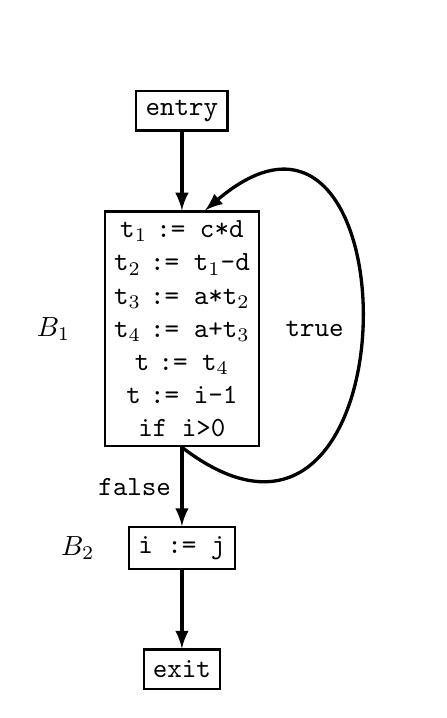
\begin{tikzpicture}[
    CFG/.style={rectangle, draw=black!100, fill=white!100, thick, minimum size=5mm, align=center},
    ]
        \node[CFG] (B0) {$\texttt{t}_1\ \texttt{:= c*d}$\\
                         $\texttt{t}_2\ \texttt{:= t}_1\texttt{-d}$\\
                         $\texttt{t}_3\ \texttt{:= a*t}_2$\\
                         $\texttt{t}_4\ \texttt{:= a+t}_3$\\
                         $\texttt{t}\ \texttt{:= t}_4$\\
                         $\texttt{t}\ \texttt{:= i-1}$\\
                         \texttt{if i>0}};
        \node[CFG, above = of B0] (start) {\texttt{entry}};
        \node[left = 3mm of B0] {$B_1$};
        
        \node[CFG] (B1) [below=of B0] {$\texttt{i := j}$};
        \node[left = 3mm of B1] {$B_2$};
        \node[CFG, below = of B1] (stop) {\texttt{exit}};
        
        \node[right = 0.2cm of B0] {\texttt{true}};
        \coordinate[above right = 2.3cm and 2cm of B0] (a) {};
        \coordinate[below right = 2.3cm and 2cm of B0] (b) {};

        \draw[-latex, very thick] (B0.south) to node[left] {\texttt{false}} (B1.north);
        \draw[-latex, very thick] (B0.south) .. controls (b) and (a)  .. ([xshift=-7mm] B0.north east);
        \draw[-latex, very thick] (start) -- (B0.north);
        \draw[-latex, very thick] (B1.south) -- (stop);
    \end{tikzpicture}
    \caption{Grafo de controle de fluxo equivalente gerado a partir da árvore da Figura \ref{fig:ast}.}
    \label{fig:cfg-exemplo}
\end{figure}

Devido à natureza da representação intermediária, os valores intermediários computados no cálculo de expressões aritméticas complexas e avaliação de estruturas de controle são expostos na forma de variáveis temporárias, que se juntam às variáveis definidas pelo programador para formar o conjunto dos valores em memória utilizados pelo programa. Esses valores são denominados registradores virtuais, e é trabalho do alocador decidir onde eles serão armazenados \cite{muchnick:97}.

Os registradores virtuais são endereços simbólicos que serão traduzidos em endereços reais após o processo de alocação de registradores. Eles são gerados de maneira incremental pelo compilador de modo a substituir os endereços reais, para possibilitar uma representação abstrata do programa na forma de código de três endereços e permitir a realização de inúmeras otimizações, sem que a disposição dos endereços de memória seja um entrave para a manipulação da IR \cite{muchnick:97}.

\section{\textit{Liveness Analysis} e Interferências}

Em posse de uma representação intermediária contendo registradores virtuais, o compilador prossegue para a tarefa de mapeá-los para endereços de memória ou registradores físicos. Como dois valores de memória não podem ocupar um único registrador físico ao mesmo tempo, o número de registradores de uso geral disponibilizados pela arquitetura-alvo pode vir a tornar-se um empecilho caso o número de variáveis seja grande demais. Os processadores x86-64 fabricados por companhias como Intel e AMD, por exemplo, possuem comumente 16 registradores de uso geral \cite{amd:06}; arquiteturas RISC como ARMv8, MIPS e SPARC apresentam respectivamente 31, 30 e 32 registradores \cite{elkady:14}.

Sendo assim, para corretamente alocar os recursos de memória da CPU de modo a comportar as variáveis utilizadas pelo programa, o compilador deve computar os pontos de utilização dos valores ao longo do programa e determinar quando uma variável está viva ou não. Esse processo é denominado análise de longevidade, ou \textit{liveness analysis}, e é uma variação da análise de fluxo de dados também efetuada em outras otimizações. 

\begin{figure}[hb]
    \centering
    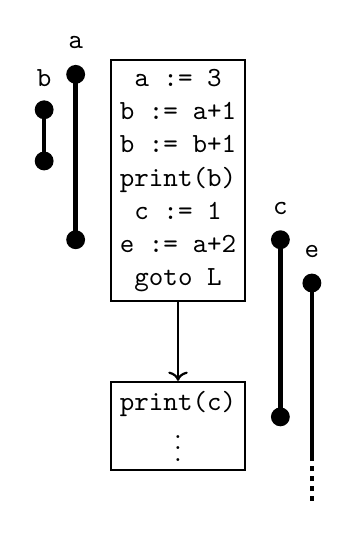
\begin{tikzpicture}[
    CFG/.style={rectangle, draw=black!100, fill=white!100, thick, minimum size=5mm, align=center},
    ]
        \node[CFG] (B0) {$\texttt{a := 3}$\\
                         $\texttt{b := a+1}$\\
                         $\texttt{b := b+1}$\\
                         $\texttt{print(b)}$\\
                         $\texttt{c := 1}$\\
                         $\texttt{e := a+2}$\\
                         \texttt{goto L}};
        \node[CFG] (B1) [below=of B0] {$\texttt{print(c)}$\\$\vdots$};
        \draw[->, thick] (B0.south) -- (B1.north);
        
        \draw[black, ultra thick] (-1.3, -0.75) -- (-1.3, 1.35);
        \filldraw[black, thick] (-1.3, -0.75) circle (3pt);
        \filldraw[black, thick] (-1.3, 1.35) circle (3pt);
        \node at (-1.3, 1.75) {$\texttt{a}$};
        
        \draw[black, ultra thick] (-1.7, 0.25) -- (-1.7, 0.90);
        \filldraw[black, thick] (-1.7, 0.25) circle (3pt);
        \filldraw[black, thick] (-1.7, 0.90) circle (3pt);
        \node at (-1.7, 1.30) {$\texttt{b}$};

        \draw[black, ultra thick] (1.3, -0.75) -- (1.3, -3);
        \filldraw[black, thick] (1.3, -0.75) circle (3pt);
        \filldraw[black, thick] (1.3, -3) circle (3pt);
        \node at (1.3, -0.35) {$\texttt{c}$};

        \draw[black, ultra thick] (1.7, -1.3) -- (1.7, -3.5);
        \filldraw[black, thick] (1.7, -1.3) circle (3pt);
        \draw[black, ultra thick, dotted] (1.7, -3.5) -- (1.7, -4.10);
        \node at (1.7, -0.9) {$\texttt{e}$};
    \end{tikzpicture}
    \caption{Dois blocos básicos contendo as variáveis \texttt{a}, \texttt{b}, \texttt{c} e \texttt{e}, com seus respectivos \textit{live ranges} indicados.}
    \label{fig:liverange-exemplo}
\end{figure}

Uma variável é dita viva no ponto que antecede diretamente a execução de uma instrução se ela contém um valor que será utilizado futuramente ou, em outra palavras, se ela será lida antes da próxima redefinição de seu valor. O conjunto de todos os pontos pelos quais uma variável contendo um valor está viva é chamado de \textit{live range}. Entretanto, uma única variável pode ser quebrada em vários \textit{live ranges}, conforme o valor que ela armazena não será mais utilizado ou é redefinido, dando origem a objetos alocáveis distintos \cite{aho:07}.

Quando dois \textit{live ranges} $v_i$ e $v_j$ se sobrepõe em determinado ponto, diz-se que há uma interferência entre eles. Em outras palavras, eles interferem pois a intersecção entre seus conjuntos de pontos não é vazia. Isso significa que ambos os valores presentes em $v_i$ e $v_j$ não podem ser mapeados para o mesmo registrador físico, pois ambos devem ser mantidos em memória integralmente para algum uso posterior. A Figura \ref{fig:liverange-exemplo} mostra dois blocos básicos com variáveis e seus respectivos \textit{live ranges}. Nesse exemplo, a variável $a$ interfere com as variáveis $b$ e $c$.

Se dois \textit{live ranges} $v_i$ e $v_j$ estiverem conectados por uma instrução de cópia na forma $v_i := v_j$ e não interferirem entre si, os dois valores podem ser armazenados no mesmo registrador. Esse ato é denominado coalescimento, ou \textit{coalescing}, e pode promover um ganho significativo na qualidade do código gerado ao eliminar instruções de cópia desnecessárias \cite{appel:96, chaitin:82, briggs:92}.

\section{Geração de Código \textit{Spill}}

O número de registradores físicos necessários para comportar os \textit{live ranges} em um ponto do código é uma métrica conhecida como pressão de registradores \cite{braun:09}. Quando esse número excede a quantidade de registradores disponíveis para a alocação, faz-se necessário armazenar algum \textit{live range} na memória principal. Para isso, são introduzidas as instruções de acesso a memória \texttt{store}, para escrever, e \texttt{load} para recuperar um valor em memória. 

\begin{figure}[hb]
    \centering
    \begin{subfigure}{0.3\textwidth}
        \centering
        \adjustbox{valign=c}{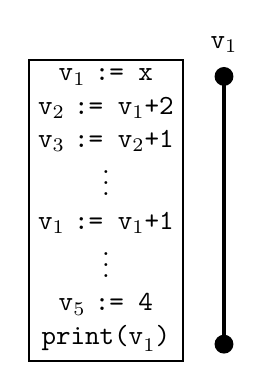
\begin{tikzpicture}[
        CFG/.style={rectangle, draw=black!100, fill=white!100, thick, minimum size=5mm, align=center},
        ]
            \node[CFG] (B0) {$\texttt{v}_1\ \texttt{:= x}$\\
                            $\texttt{v}_2\ \texttt{:= v}_1\texttt{+2}$\\
                            $\texttt{v}_3\ \texttt{:= v}_2\texttt{+1}$\\
                            $\vdots$\\
                            $\texttt{v}_1\ \texttt{:= v}_1\texttt{+1}$\\
                            $\vdots$\\
                            $\texttt{v}_5\ \texttt{:= 4}$\\
                            $\texttt{print(v}_1\texttt{)}$};
            
            \draw[black, ultra thick] (1.5, -1.70) -- (1.5, 1.70);
            \filldraw[black, thick] (1.5, -1.70) circle (3pt);
            \filldraw[black, thick] (1.5, 1.70) circle (3pt);
            \node at (1.5, 2.10) {$\texttt{v}_1$};
        \end{tikzpicture}}
    \end{subfigure}
    \begin{subfigure}{0.1\textwidth}
        \centering
        \adjustbox{valign=c}{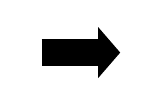
\begin{tikzpicture}
            \draw[-{Triangle[width=18pt,length=8pt]}, line width=10pt] (0,5) -- (1,5);
        \end{tikzpicture}}
    \end{subfigure}
    \begin{subfigure}{0.3\textwidth}
        \centering
        \adjustbox{valign=c}{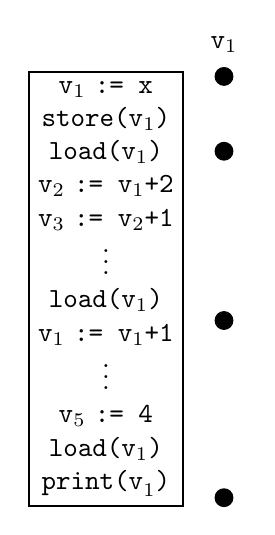
\begin{tikzpicture}[
        CFG/.style={rectangle, draw=black!100, fill=white!100, thick, minimum size=5mm, align=center},
        ]
            \node[CFG] (B0) {$\texttt{v}_1\ \texttt{:= x}$\\
                             $\texttt{store(v}_1\texttt{)}$\\
                             $\texttt{load(v}_1\texttt{)}$\\
                             $\texttt{v}_2\ \texttt{:= v}_1\texttt{+2}$\\
                             $\texttt{v}_3\ \texttt{:= v}_2\texttt{+1}$\\
                             $\vdots$\\
                             $\texttt{load(v}_1\texttt{)}$\\
                             $\texttt{v}_1\ \texttt{:= v}_1\texttt{+1}$\\
                             $\vdots$\\
                             $\texttt{v}_5\ \texttt{:= 4}$\\
                             $\texttt{load(v}_1\texttt{)}$\\
                             $\texttt{print(v}_1\texttt{)}$};
            
            % \draw[black, ultra thick] (1.5, 2.70) -- (1.5, -1.70);
            \node at (1.5, 3.1) {$\texttt{v}_1$};
            \filldraw[black, thick] (1.5, 2.70) circle (3pt);
            \filldraw[black, thick] (1.5, 1.75) circle (3pt);
            \filldraw[black, thick] (1.5, -0.4) circle (3pt);
            \filldraw[black, thick] (1.5, -2.65) circle (3pt);
        \end{tikzpicture}}
    \end{subfigure}
    \caption{Exemplo de bloco básico antes e depois do \textit{spill} do \textit{live range} $\texttt{v}_1$.}
    \label{fig:spill-exemplo}
\end{figure}

Essas instruções são denominadas código \textit{spill}, e tem por efeito fragmentar o \textit{live range} escolhido ao redor do ponto de grande pressão, a fim de reduzi-la \cite{chaitin:81}. Ao longo do curso de execução de um programa, uma mesma variável pode ser ser armazenada em registradores e posteriormente ser enviada para a memória, e ter seu \textit{live range} particionado \cite{eisl:16}. A Figura \ref{fig:spill-exemplo} mostra um bloco básico antes e depois do \textit{spill} da variável $v_1$, cujo tempo de vida é decomposto em várias porções menores, aliviando a pressão em determinados pontos.

Esse artifício, no entanto, produz um código mais lento. As instruções de acesso à memória consomem significativamente mais ciclos do que operações aritméticas simples em registradores e desvios. A inserção de \textit{spill code} em locais inapropriados, como em laços de repetição ou trechos que serão frequentemente executados, podem causar um grande \textit{overhead} que derruba a performance do executável gerado. Um alocador eficiente tem a tarefa de minimizar a quantidade de acessos à memória gerados o quanto for possível, e ser preciso em suas escolhas sobre quais variáveis selecionar para \textit{spill} e a colocação das instruções.

\section{Alocação via Coloração de Grafos}

A alocação de registradores por coloração de grafos é a abordagem dominante para o desenvolvimento de alocadores na atualidade. Ela foi implementada pela primeira vez por Chaitin \textit{et al.} em 1980, em um compilador experimental da linguagem PL/I para o IBM System/370 \cite{chaitin:81}, e foi o primeiro método amplamente aplicado para alocação global de registradores, onde os registradores são alocados para toda a unidade de compilação (função) de uma só vez, em vez de alocá-los por bloco \cite{eisl:16}.

\begin{figure}[hbt]
    \centering
    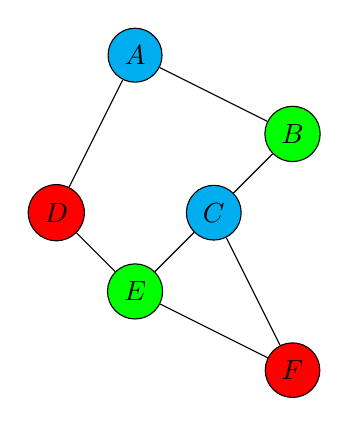
\begin{tikzpicture}

        % Definindo vértices    
        \foreach \pos/\name/\color in {{(0,2)/A/cyan}, {(2,1)/B/green}, {(1,0)/C/cyan},
                                       {(-1,0)/D/red}, {(0,-1)/E/green}, {(2,-2)/F/red}}
            \node[circle, fill=\color, draw=black] (\name) at \pos {$\name$};
        
        % Definindo arestas
        \foreach \source/\target in {A/B, B/C, C/F, D/A, E/C, F/E, D/E}
            \draw (\source) -- (\target);
    
    \end{tikzpicture}
    
    \caption{Exemplo de grafo de interferência colorido com três cores.}
    \label{fig:grafo-petersen}
\end{figure}

Seja $G = (V, E)$ um grafo não-direcionado, onde os vértices $v \in V$ representam os \textit{live ranges} e as arestas $e \in E$ as interferências, tal que $e = (v_i, v_j)$ simboliza a existência de uma interferência entre $v_i$ e $v_j$. O grafo $G$ é dito $k$-colorível se houver uma função $cor: V \to \{1,...,k\}$ tal que $cor(v_i) \ne cor(v_j)$, para todo $v_i$ e $v_j$ em que existir uma aresta
$e_n = (v_i, v_j)$. A alocação é reduzida, então, a encontrar o mapeamento dado pela função $cor$, onde $k$ é o número de registradores físicos presentes na arquitetura-alvo.

Entretanto, computar uma solução ótima não é trivial. A coloração de grafo é um clássico problema NP-completo \cite{karp:72} --- determinar a $k$-colorabilidade de um grafo possui complexidade exponencial e logo torna-se inviável para casos que envolvem muitos registradores virtuais \cite{lawler:76, bjorklund:09}, e a mera tarefa de determinar o número mínimo de cores para se colorir um grafo é um problema NP-\textit{hard} \cite{garey:76}. A Figura \ref{fig:grafo-petersen} exibe uma possível instância de grafo de interferência, formado pelas variáveis $A$, $B$, $C$, $D$, $E$ e $F$, e colorido com três cores.

\subsection{Alocador de \textit{Chaitin}}

Chaitin \textit{et al.} \cite{chaitin:82} formalizaram, em 1982, seu algoritmo de alocação global de registradores via coloração de grafo. A Figura \ref{fig:alocador-chaitin} esquematiza a execução do alocador, que consiste em construir um grafo de interferência e manipulá-lo em etapas que estão descritas a seguir:

\begin{enumerate}
    \item \textit{\textbf{Renumber}} --- encontrar todos os \textit{live ranges} dentro do escopo da função ou procedimento, e lhes atribuir um identificador único;
    \item \textit{\textbf{Build}} --- construir o grafo de interferência $G = (V,E)$, onde cada \textit{live range} se torna um vértice $v\in 
    V$ e as arestas $(v_i,v_j)\in E$ são adicionadas conforme o código é varrido de maneira retrógrada e as interferências são descobertas;
    \item \textit{\textbf{Coalesce}} --- combinar os \textit{live ranges} que são conectados por uma única instrução de cópia $v_i:=v_j$ e não interferem entre si, de modo que os vértices correspondentes no grafo sejam combinados em um único vértice $v_{ij}$. A instrução de cópia pode ser removida da IR, e as etapas de \textit{build} e \textit{\textbf{coalesce}} devem ser refeitas devido à modificação no código;
    \item \textit{\textbf{Spill cost}} --- computar o custo de \textit{spill} para cada \textit{live range}. Esse custo é uma estimativa do aumento no tempo de execução se um dado vértice for mapeado para a memória principal, aumento esse que é proporcional ao número de vezes que as instruções de \texttt{store} e \texttt{load} inseridas serão executadas;
    \item \textit{\textbf{Simplify}} --- remover os vértices tal que $grau(v)<k$, onde $grau(v)$ é o número de arestas de $v$ e $k$ é número de cores. Isso pode ser feito pois, se um vértice possui um número de arestas menor do que o número de cores, ele certamente é colorível. Sendo assim, após a remoção, o vértice deve ser adicionado a uma pilha auxiliar $S$, que serve como estrutura de controle da ordem de remoção.
    
    Se não houverem vértices aptos a serem removidos, algum deve ser escolhido para sofrer \textit{spill}. A prioridade de \textit{spill} é calculada utilizando o custo calculado na etapa anterior, sendo igual a $custo(v)/grau(v)$. O vértice que apresentar o menor custo então é escolhido e a etapa \textit{spill code} é acionada; 
    \item \textit{Spill code} --- o código é alterado com a inserção de instruções de acesso à memória, e o algoritmo deve reiniciar a partir da etapa \textit{renumber};
    \item \textit{Select} --- assinalar cores aos vértices de $G$, os desempilhando de $S$ um a um, na ordem reversa à que foram removidos na etapa anterior. Se a geração de \textit{spill code} não foi acionada, seguramente todos os vértices receberão uma cor tal que $cor(v_i)\ne cor(v_j)$ onde $v_i$ e $v_j$ são vizinhos.
\end{enumerate}

\begin{figure}
    \centering
    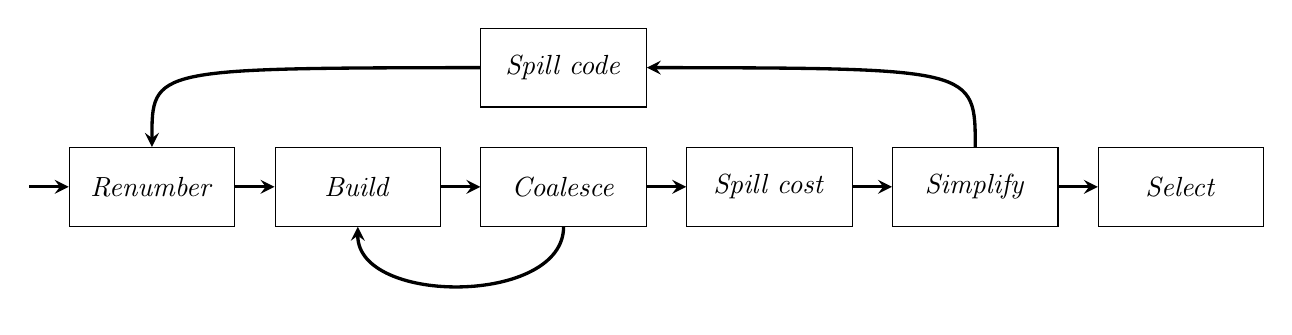
\begin{tikzpicture}[
        node distance= 1cm and 0.5cm,
        box/.style={draw, rectangle, minimum width=2.1cm, minimum height=1cm, align=center},
        arrow/.style={very thick, ->, >=stealth},
    ]
        \node[box] (renumber) {\textit{Renumber}};
        \node[box, right = of renumber] (build) {\textit{Build}};
        \node[box, right = of build] (coalesce) {\textit{Coalesce}};
        \node[box, right = of coalesce] (cost) {\textit{Spill cost}};
        \node[box, right = of cost] (simplify) {\textit{Simplify}};
        \node[box, right = of simplify] (select) {\textit{Select}};
        \node[box, above = 0.5cm of coalesce] (spill) {\textit{Spill code}};
        \coordinate[above = of simplify] (bezier1);
        \coordinate[above = of renumber] (bezier2);
        \coordinate[below = of coalesce] (bezier3);
        \coordinate[below = of build] (bezier4);
        \coordinate[left = of renumber] (start);

        \draw[arrow] (renumber) -- (build);
        \draw[arrow] (build) -- (coalesce);
        \draw[arrow] (coalesce) -- (cost);
        \draw[arrow] (cost) -- (simplify);
        \draw[arrow] (simplify) -- (select);

        \draw[arrow] (simplify.north) .. controls (bezier1) .. (spill.east);
        \draw[arrow] (spill.west) .. controls (bezier2) .. (renumber.north);
        \draw[arrow] (coalesce.south) .. controls (bezier3) and (bezier4) .. (build.south);
        \draw[arrow] (start) -- (renumber.west);
    \end{tikzpicture}
    \caption{Esquema do algoritmo de Chaitin \cite{chaitin:82}.}
    \label{fig:alocador-chaitin}
\end{figure}

\subsection{Alocador de \textit{Chaitin-Briggs}}

Briggs \cite{briggs:92} propôs uma série de alterações ao algoritmo de Chaitin a fim de corrigir uma série de defeitos que sua versão inicial apresentava. Notavelmente, ele sugeriu um atraso na etapa de geração de \textit{spill code} para produzir alocações mais eficientes e alguns ajustes no processo de coalescimento do alocador, a fim de otimizar o tratamento de instruções de cópia.

Em um trabalho anterior, de 1989 \cite{briggs:89}, Briggs \textit{et al.} demonstraram que o alocador de Chaitin era ineficiente na sua etapa de \textit{simplify}, ao gerar \textit{spill} em grafos que são trivialmente coloríveis. Um exemplo usado pelo próprio Briggs é o de um grafo em forma de losango, possuindo quatro vértices com duas arestas cada e que é visivelmente colorível para um número de cores $k=2$, como mostrado na Figura \ref{fig:grafo-diamante}. No entanto, o alocador de Chaitin fatalmente enviaria algum registrador virtual para a memória pois, na etapa de \textit{simplify}, não haveriam vértices tal que $\mathit{grau}(v)<2$ e algum deles e a ativação da etapa \textit{spill code} seria imediata.

\begin{figure}[ht]
    \centering
    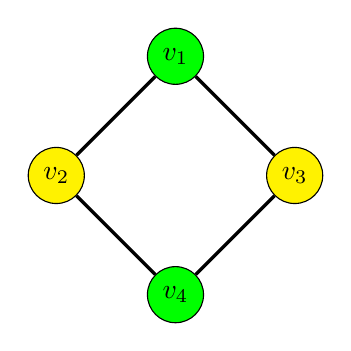
\begin{tikzpicture}[node/.style={draw,circle}]
        \node[node, fill=green] (v_1) {$v_1$};
        \node[node, below left = of v_1, fill=yellow] (v_2) {$v_2$};
        \node[node, below right = of v_1, fill=yellow] (v_3) {$v_3$};
        \node[node, below left = of v_3, fill=green] (v_4) {$v_4$};
        
        \draw[-, very thick] (v_1) -- (v_2);
        \draw[-, very thick] (v_2) -- (v_4);
        \draw[-, very thick] (v_3) -- (v_4);
        \draw[-, very thick] (v_3) -- (v_1);
        
    \end{tikzpicture}
    \caption{Grafo $2$-colorível que seria incorretamente colorido pelo alocador de Chaitin.}
    \label{fig:grafo-diamante}
\end{figure}

Para solucionar o problema da realização precipitada de \textit{spill}, Briggs propôs adiar a etapa de \textit{spill code} para depois da etapa de \textit{select}. Assim, se por acaso não houverem vértices aptos a serem removidos durante a fase de simplificação, é escolhido um candidato a \textit{spill} dentre os vértices cujo grau é maior que o número de cores $k$. Por ser somente um candidato, o alocador ainda deve considerar a possibilidade de colorir esse vértice no futuro e ele pode portanto ser removido do grafo, permitindo destravar o algoritmo e continuar a etapa de \textit{simplify}. 

Posteriormente, na etapa de \textit{select}, será avaliada a necessidade de se efetuar \textit{spill} das variáveis candidatas: se ao desempilhar um vértice $v$ tal que $\mathit{grau}(v)>k$ não for possível encontrar uma cor para $v$, somente então a geração de \textit{spill} code é ativada. Dessa forma, o alocador torna-se capaz de colorir vértices cujo número de arestas é maior do que o número de cores disponíveis, preservando a ordem de coloração produzida pelo alocador de Chaitin. Esssa técnica foi denominada \textit{optimistic coloring}, e é ilustrada pela Figura \ref{fig:alocador-briggs}, exibindo o fluxo básico de execução de um alocador ao estilo de Briggs.

Além disso, o algoritmo de Chaitin, na etapa de \textit{coalesce}, poderia transformar um grafo $k$-colorível em um não-colorível ao combinar dois vértices $v_i$ e $v_j$ em um único vértice $v_{ij}$, onde $grau(v_{ij})\geq k$. Dessa forma, Briggs \textit{et al.} \cite{briggs2:92} propuseram o \textit{conservative coalescing}, que consiste em somente coalescer dois vértices se a união de ambos tiver um grau menor do que o número de cores, sendo assim garantidamente colorível.

\begin{figure}[hb]
    \centering
    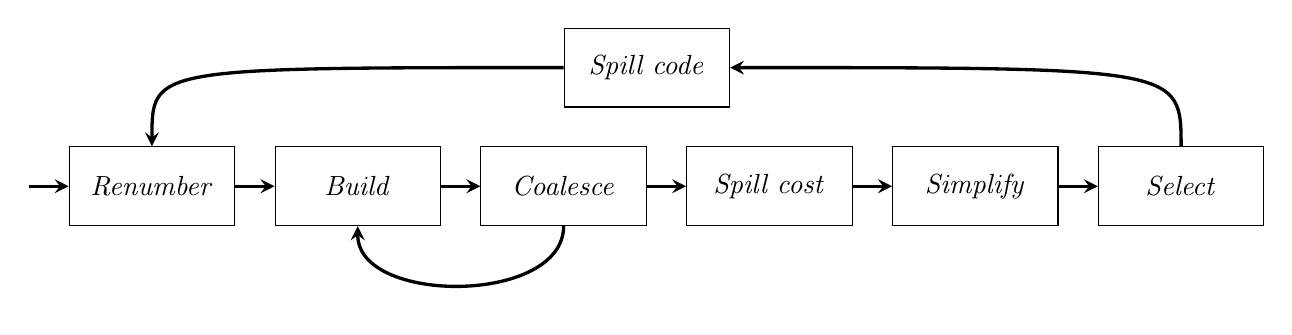
\begin{tikzpicture}[
        node distance= 1cm and 0.5cm,
        box/.style={draw, rectangle, minimum width=2.1cm, minimum height=1cm, align=center},
        arrow/.style={very thick, ->, >=stealth},
    ]
        \node[box] (renumber) {\textit{Renumber}};
        \node[box, right = of renumber] (build) {\textit{Build}};
        \node[box, right = of build] (coalesce) {\textit{Coalesce}};
        \node[box, right = of coalesce] (cost) {\textit{Spill cost}};
        \node[box, right = of cost] (simplify) {\textit{Simplify}};
        \node[box, right = of simplify] (select) {\textit{Select}};
        \coordinate[above = of select] (bezier1);
        \coordinate[above = of renumber] (bezier2);
        \coordinate[below = of coalesce] (bezier3);
        \coordinate[below = of build] (bezier4);
        \coordinate[left = of renumber] (start);
        \coordinate[above = of cost] (d);
        \node[box, left = of d] (spill) {\textit{Spill code}};

        \draw[arrow] (renumber) -- (build);
        \draw[arrow] (build) -- (coalesce);
        \draw[arrow] (coalesce) -- (cost);
        \draw[arrow] (cost) -- (simplify);
        \draw[arrow] (simplify) -- (select);

        \draw[arrow] (select.north) .. controls (bezier1) .. (spill.east);
        \draw[arrow] (spill.west) .. controls (bezier2) .. (renumber.north);
        \draw[arrow] (coalesce.south) .. controls (bezier3) and (bezier4) .. (build.south);
        \draw[arrow] (start) -- (renumber.west);
    \end{tikzpicture}
    \caption{Esquema do algoritmo de Briggs, com a etapa de geração de \textit{spill code} adiada.}
    \label{fig:alocador-briggs}
\end{figure}

\subsection{\textit{Iterated Register Coalescing}}

Em 1996, George e Appel \cite{appel:96} propuseram uma maneira diferente de coalescer os registradores virtuais: o \textit{iterated register coalescing} é um método mais agressivo de combinar vértices no grafo de interferência, sem adicionar novos \textit{spills} desnecessariamente. Ele consistia em executar as etapas de \textit{simplify} e \textit{coalesce} iterativamente, com a inclusão de uma etapa adicional denominada \textit{freeze}, como descrito a seguir:

\begin{enumerate}
    \item \textit{\textbf{Build}} --- construir o grafo de interferência e categorizar cada vértice como relacionado a \texttt{move} ou não. Um vértice relacionado a \texttt{move} é aquele que é a origem ou o destino de uma instrução de \texttt{move};
    \item \textit{\textbf{Simplify}} --- realizar a remoção dos vértices não-relacionados a \texttt{move}, com grau menor do que o número de cores;
    \item \textit{\textbf{Coalesce}} --- combinar vértices ao estilo de Briggs no grafo reduzido obtido da fase anterior. Como os graus de muitos nós já foram reduzidos pela simplificação, provavelmente haverão muito mais vértices válidos para serem coalescidos do que no grafo de inicial. Após dois vértices $v_i$ e $v_j$ terem sido unidos (e a instrução de \texttt{move} excluída), se $v_{ij}$ não for mais relacionado a \texttt{move}, ele estará apto a ser removido na próxima rodada do \textit{simplify}. Essa etapa e a anterior são repetidas até que restem apenas vértices tal que $grau(v)\geq k$ ou relacionados a \texttt{move}.
    \item \textit{\textbf{Freeze}} --- caso nem \textit{simplify}, nem \textit{coalesce} se aplicarem, um vértice de menor grau é escolhido para tornar-se não-relacionado a \texttt{move}, e apto a sofrer simplificação. Agora, \textit{simplify} e \textit{coalesce} são retomados.
    \item \textit{\textbf{Select}} --- assinalar cores aos vértices, de maneira similar ao método de Briggs.
\end{enumerate}

O \textit{iterated register coalescing} representa o estado da arte da alocação de registradores via coloração de grafos, sendo o algoritmo de referência para os compiladores de produção, bem como os ligados à pesquisa \cite{protzenko:09}. A Figura \ref{fig:iterated-register-coalescing} apresenta um esquema do funcionamento do alocador de George e Appel:

\begin{figure}[hbt]
    \centering
    \begin{tikzpicture}[
        node distance= 1cm and 0.5cm,
        box/.style={draw, rectangle, minimum width=2.1cm, minimum height=1cm, align=center},
        arrow/.style={very thick, ->, >=stealth},
    ]
        \node[box] (build) {\textit{Build}};
        \node[box, right = of build] (simplify) {\textit{Simplify}};
        \node[box, right = of simplify] (coalesce) {\textit{Coalesce}};
        \node[box, right = of coalesce] (freeze) {\textit{Freeze}};
        \node[box, right = of cost] (potspill) {\textit{Potencial spill}};
        \node[box, right = of potspill] (select) {\textit{Select}};

        % \draw[arrow] (simplify.150) .. controls ([yshift=5mm] simplify.150) and ([yshift=5mm] simplify.120) .. (simplify.120);
        \draw[arrow] (build) -- (simplify);
        \draw[arrow] (simplify) -- (coalesce);
        \draw[arrow] (coalesce) -- (freeze);
        \draw[arrow] (freeze) -- (potspill);
        \draw[arrow] (potspill) -- (select);
        \draw[arrow] (freeze.south) .. controls ([yshift=-14mm] freeze.south) and ([yshift=-14mm] simplify.south) .. (simplify.south); 

        \draw[arrow] (coalesce.south) .. controls ([yshift=-7mm] coalesce.south) and ([yshift=-7mm] simplify.300) .. (simplify.300);
        \draw[arrow] (potspill.south) .. controls ([yshift=-21mm] potspill.south) and ([yshift=-21mm] simplify.240) .. (simplify.240);

        \node[box] (spill) at ([yshift=2.5cm] current bounding box.center) {\textit{Spill code}};

        \draw[arrow] (select.north) .. controls ([yshift=10mm] select.north) and ([xshift=4mm] spill.east) .. (spill.east);
        \draw[arrow] (spill.west) .. controls ([xshift=-4mm] spill.west) and ([yshift=10mm] build.north) .. (build.north);
    \end{tikzpicture}
    \caption{Esquema do Iterated Register Coalescing, apresentando a etapa de \textit{freeze}.}
    \label{fig:iterated-register-coalescing}
\end{figure}

\section{Alocação via \textit{Linear Scan}}

Um paradigma de alocação de registradores alternativo à coloração de grafos é o da alocação via \textit{linear scan}, que foi proposta pela primeira vez por Poletto e Sarkar \cite{poletto:99}. Dados os \textit{live ranges} presentes no escopo de uma função, ao invés de construir um grafo de interferência o algoritmo efetua uma única varredura, na ordem de uma enumeração arbitrária da IR, alocando os registradores físicos através de uma estratégia gulosa. 

O algoritmo de \textit{linear scan} é simples, eficiente e produz código comparável ao produzido via coloração de grafos, com a vantagem de propiciar um tempo de compilação consideravelmente mais rápido. Isso pois o algoritmo de \textit{linear scan} apresenta uma complexidade linear, em contrapartida à abordagem por coloração de grafos que tem complexidade quadrática \cite{johansson:01}. Dessa forma, para compiladores onde a velocidade de compilação é uma prioridade, como em compiladores \textit{just-in-time} (JIT) ou interpretadores em tempo real, a alocação via \textit{linear scan} configura-se como a melhor opção.

A técnica de \textit{linear scan} aproxima o conceito de \textit{live range} na forma de intervalos vivos, ou \textit{live intervals}. Dada alguma enumeração da representação intermediária, $[i,j]$ é um \textit{live interval} de $v$ se não houverem instruções de número $i'<i$ e $j'>j$, tal que $v$ esteja viva em $i'$ e $j'$. Podem haver subintervalos de $[i,j]$ onde $v$ não está viva, mas eles são ignorados para todos os fins. Os \textit{live intervals} de um programa podem ser facilmente computados por meio de uma única passagem pelo código, e as interferências entre eles são determinadas pela existência de sobreposições entre os intervalos. O Algoritmo \ref{alg:linearscan} apresenta o pseudocódigo do \textit{linear scan}, como mostrado em Poletto e Sarkar \cite{poletto:99}.

O algoritmo consiste em percorrer os intervalos $[i,j]$ em ordem crescente a partir do ponto inicial do intervalo $i$, atribuindo os registradores físicos disponíveis para cada um deles. Uma lista de ativos $A$ é mantida ordenada em ordem crescente dos pontos finais dos intervalos $j$, e armazena os \textit{live intervals} que se sobrepõe com o ponto atual e foram armazenados em registradores. A cada passo, o procedimento varre $A$ removendo os intervalos ``expirados'', cujo ponto final precede o ponto inicial do atual intervalo em análise e o registrador correspondente é marcado como livre para ser alocado. O algoritmo então tenta encontrar um registrador disponível para o atual intervalo e, caso não haja nenhum, \textit{spill} deve ser realizado.

\begin{figure}[ht]
    \centering
    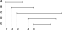
\includegraphics[scale=1.3]{linearscan}
    \caption{Exemplo de um conjunto de cinco \textit{live intervals}. Extraído de Poletto e Sarkar \cite{poletto:99}.}
    \label{fig:linearscan}
\end{figure}

\begin{figure}[hb]
    \centering
    \includegraphics[scale=1.2]{linearscan-comum}
    \caption{Exemplo em pseudocódigo mostrando os \textit{live intervals} no \textit{linear scan} tradicional. Figura extraída de Wimmer \textit{et al.} \cite{wimmer:04}.}
    \label{fig:liveintervals-normal}
\end{figure}

Entretanto, o \textit{linear scan} como proposto por Poletto e Sarkar apresenta duas grandes desvantagens. Em primeiro lugar, devido ao seu aspecto guloso, o algoritmo não leva em consideração ``lacunas'' nos \textit{live intervals}, isto é, subintervalos onde o valor da variável não é usado e não precisa ser armazenado. Além disso, uma variável enviada para memória permanecerá em memória durante todo o seu tempo de vida \cite{eisl:16}.

Em 1998, Traub \textit{et al.} \cite{traub:98} propuseram uma versão aprimorada do algoritmo de \textit{linear scan} que realiza a alocação e reescreve o código em uma única varredura no código. No \textit{second-chance binpacking}, o conceito de intervalo é refinado e alcança a mesma precisão dos \textit{live ranges} propriamente ditos, possibilitando aproveitar as lacunas presentes em meio aos \textit{live intervals}. Ao buscar um registrador para uma nova variável, o alocador pode verificar a existência de lacunas nos intervalos previamente alocados e escolher a menor lacuna de tamanho suficiente para comportar o novo \textit{live interval}, reutilizando o mesmo registrador físico. As Figuras \ref{fig:liveintervals-normal} e \ref{fig:liveintervals-binpacking} mostram exemplos do método tradicional e da melhoria de Traub \textit{et al}., respectivamente.

\begin{figure}
    \centering
    \includegraphics[scale=1.2]{linearscan-binpacking}
    \caption{O mesmo exemplo da Figura \ref{fig:liveintervals-normal} com os \textit{live intervals} do \textit{second-chance binpacking}, e a alocação de registradores final. Extraído de Wimmer \cite{wimmer:04}.}
    \label{fig:liveintervals-binpacking}
\end{figure}

\begin{algoritmo}[H]
    \caption{Algoritmo do \textit{linear scan}. Adaptado de Poletto e Sarkar \cite{poletto:99}.}
    \begin{algorithmic}
        \Require $A$: lista de ativos, $R$: conjunto de registradores físicos, $I$: conjunto de \textit{live intervals}
        \Procedure{LinearScan}{}
            \State $A \gets \{\}$, ordenado em ordem crescente de pontos finais
            \State $\mathit{livres} \gets R$
            \ForAll{\textit{live interval} $i \in I$}
                \State \Call{ExpirarIntervalos} {$i, A$}
                \State $A \gets A \cup \{i\}$
                \If{$|A| < |R|$}
                    \State $\mathit{registrador}[i] \gets$ um registrador $r \in \mathit{livres}$
                    \State $\mathit{livres} \gets \mathit{livres} - \{r\}$
                \Else \State \Call{Spill} {$i, A$}
                \EndIf
            \EndFor
        \EndProcedure
        
        \Function{ExpirarIntervalos}{$i, A$}
            \ForAll{\textit{live interval} $a \in A$}
                \If{$\mathit{fim}[a] \geq \textit{inicio}[i]$}
                    \State \Return
                \EndIf
                \State $A \gets A-\{a\}$
                \State $\mathit{livres} \gets \textit{livres} \cup \{\mathit{registrador}[a]\}$
            \EndFor
        \EndFunction
        
        \Function{Spill}{$i, A$}
            \State $\mathit{spill} \gets$ último \textit{live interval} em $A$
            \If{$\mathit{fim}[\textit{spill}] > \textit{fim}[i]$}
                \State $\mathit{registrador}[i] \gets \mathit{registrador}[\mathit{spill}]$
                \State $\mathit{spill}$ é enviado para a memória principal
                \State $A \gets A - \{\mathit{spill}\}$
            \Else
                \State $\mathit{spill}$ é enviado para a memória principal
            \EndIf
        \EndFunction
    \end{algorithmic}
    \label{alg:linearscan}
\end{algoritmo}

\section{Alocação via PBQP}

Em 2002, Scholz e Eckstein \cite{scholz:02} propuseram uma abordagem inovadora para a alocação de registradores valendo-se do PBQP (\textit{Partitioned Boolean Quadratic Optimization Problem}), um problema de otimização que consiste em modelar conjuntos de escolhas como equações booleanas, cada qual com uma lista de custos associados e visando encontrar a sequência de escolhas que produza o resultado com menor custo possível. Esse método de alocação consegue efetivamente combinar as tarefas do alocador e representava as peculiaridades de arquiteturas irregulares em um único problema.

Para cada registrador simbólico, o alocador deve decidir se o armazena em um dos registradores $r_1$, $r_2$, $\ldots$, $r_k$, sendo $k$ o número de registradores físicos, ou se o envia para a memória principal. Essa decisão é expressa na forma de uma equação formada por uma soma de variáveis booleanas. Uma das variáveis booleanas representa a decisão de se fazer \textit{spill} do registrador virtual, enquanto as variáveis booleanas restantes representam as decisões de se alocar algum registrador da CPU à variável. A Fórmula \ref{eq:equacao-pbqp} expressa a equação booleana, onde $x_{\mathit{spill}}\in \{0,1\}$ representa a decisão de \textit{spill} e $x_{i}\in \{0,1\}$ simboliza a alocação de algum dos $k$ registradores.

\begin{equation}
    x_{\mathit{spill}} + x_{1} + x_{2} + \ldots + x_{k} = 1
    \label{eq:equacao-pbqp}
\end{equation}

Como a Equação \ref{eq:equacao-pbqp} é linear, ela pode ser representada na forma de um vetor booleano $\Vec{x_v}$. De maneira análoga, os custos de cada alocação $a$ do conjunto das possibilidades de alocação $A$, associada aos índices de $\Vec{x_v}$, compõe o vetor de custo $\Vec{c_v}$. Nesse caso, a atribuição de um registrador físico para o registrador virtual $v$ corresponde a um índice $\phi_a$ de $\Vec{x_v}$ cuja variável booleana correspondente é igual a 1, e $f_v$ é a função do custo de alocação de $v$ dentre o conjunto $F_v$, que simboliza os custos de se alocar a variável a cada um dos registradores disponíveis. A Definição \ref{eq:vetor-pbqp} mostra como $\Vec{c_v}$ é computado:

\begin{equation}
    \forall a \in A : \Vec{c_v}({\phi}_a)=\sum_{\mathclap{f_v \in F_v}}f_v(a).
    \label{eq:vetor-pbqp}
\end{equation}

Sendo assim, tem-se que cada registrador virtual tem a si associado um vetor de custos na forma $\Vec{c_v} = [110, 0, 4, \infty, \ldots, \infty]^T$. Nesse exemplo, temos que o primeiro índice é o custo de \textit{spill} da variável; os dois índices seguintes são o custo de alocação para dois registradores físicos hipotéticos. Os índices subsequentes, com custo infinito, representam possibilidades de alocação não permitidas por alguma restrição da arquitetura ou porque já estão ocupadas.

Se dois registradores virtuais $u$ e $v$ forem dependentes entre si devido a alguma interferência nos \textit{live ranges}, estiverem conectadas por uma instrução de cópia ou constituírem um par ditado pela arquitetura, o custo de alocação é expresso pela forma quadrática $\Vec{x_u}C_{uv}\Vec{x_v}^T$, mostrada na Definição \ref{eq:formula-matriz-pbqp}. 

De maneira análoga, $a_u, a_v \in A$ representam um par de alocações de registradores para $u$ e $v$ respectivamente, e ambos os índices $\phi_{a_u},\phi_{a_v}$ dos vetores de custo individuais de cada variável são levados em conta na obtenção do custo combinado $C_{uv}$. Por isso, o conjunto dos custos $C_{uv}$ assume a forma da Matriz \ref{eq:matriz-pbqp}, onde os índices de linha e coluna estão associados às decisões individuais em $u$ e $v$.

\begin{equation}
        \forall a_u, a_v \in A : C_{uv}(\phi_{a_u},\phi_{a_v}) = \sum_{\mathclap{f_{uv} \in F_{uv}}} f_{uv}(a_u,a_v)
        \label{eq:formula-matriz-pbqp}
    \end{equation}

\begin{equation}
        C_{uv} = \begin{bmatrix}
        c_{ij}
        \end{bmatrix} = \begin{bmatrix}
            0 & 0 & \ldots & 0 \\
            0 & \infty & \ddots & \vdots \\
            \vdots & \ddots & \ddots & 0 \\
            0 & \ldots & 0 & \infty
        \end{bmatrix}
        \label{eq:matriz-pbqp}
\end{equation}

Sendo assim, a tarefa de alocação é expressa na forma de um problema de particionamento quadrático, que consiste em encontrar o esquema de alocação que minimize o resultado da Fórmula \ref{eq:pbqp}.

\begin{equation}
    \text{min }f = \sum_{\mathclap{1 \leq u < v \leq k}} \Vec{x}_u C_{uv} \Vec{x}_v^T + \sum_{\mathclap{1 \leq u \leq k}} \Vec{c}_u \Vec{x}_u^T.
    \label{eq:pbqp}
\end{equation}

Na Fórmula \ref{eq:pbqp}, os índices $u$ e $v$ representam pares de registradores virtuais e $k$ é o número de registradores virtuais. Devido às propriedades simétricas das formas quadráticas, o resultado da função é uma soma triangular \footnote{Soma triangular, ou número triangular, é um número dado pela série $\sum_{k=1}^n k=1+2+3+\ldots+n=\frac{(n^2+n)}{2}$ \cite{hoggatt:74}.}. Observa-se que existe pelo menos uma solução com custo finito, desde que os custos de \textit{spill} sejam finitos. Isto se deve ao fato de que todos as variáveis podem sofrer \textit{spill}, embora não seja uma boa solução.

Ainda que o problema possa ser expresso formalmente, uma modelagem baseada em grafos é mais intuitiva. Nesse contexto, cada vértice do grafo possui um vetor de escolha associado, que atribui a cada alternativa seu custo de execução, e para cada nó apenas uma alternativa pode ser selecionada. As interdependências são modeladas por arestas direcionadas com uma matriz associada, que contém os custos das combinações de alternativas. A Figura \ref{fig:9} mostra um exemplo de representação de um problema PBQP via grafo. Cada vértice u, v e w possui três alternativas que representam suas cores possíveis. Devido às matrizes de arestas, cada solução possível deve selecionar cores diferentes para nós adjacentes e, portanto, representa uma 3-coloração válida \cite{buchwald:11}.

\begin{figure}
    \centering
    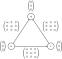
\includegraphics[scale=1.5]{pbqp}
    \caption{Grafo de resolução do PBQP considerando 3 registradores virtuais. Extraído de Buchwald \textit{et al} \cite{buchwald:11}}
    \label{fig:9}
\end{figure}

O PBQP é um problema NP-completo, de maneira similar à coloração de grafos. No entanto, soluções quase-ótimas podem ser obtidas através de técnicas como programação dinâmica e a aplicação de heurísticas de simplificação, que permitem reduzir uma instância do problema de tal modo que a melhor resolução torne-se trivial. Ao retropropagar as reduções, a seleção da instância menor pode ser estendida para uma seleção da instância original do PBQP. Originalmente, foram propostas quatro reduções \cite{buchwald:10, eckstein:03}:
\begin{enumerate}
    \item \textit{\textbf{RE}} --- remoção de arestas independentes, possuindo uma matriz de custos que pode ser decomposta em dois vetores $\Vec{u}$ e $\Vec{v}$, ou seja, cada entrada da matriz $c_{ij}$ tem custos $u_i$ + $v_j$. Essas arestas podem ser removidas ao se somar $\Vec{u}$ e $\Vec{v}$ aos vetores de custo dos vértices de origem e de destino, respectivamente. Se isto produzir custos vetoriais infinitos, a alternativa correspondente (incluindo linhas/colunas da matriz) é eliminada;

    \begin{figure}[H]
        \centering
        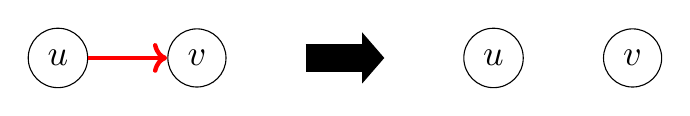
\begin{tikzpicture}[scale=1.3, node/.style={draw,circle,scale=1.3}]
            \node[node] (u1) {$u$};
            \node[node, right = of u1] (v1) {$v$};
            \coordinate[right = of v1] (a);
            \coordinate[right = of a] (b);
            \node[node, right = of b] (u2) {$u$};
            \node[node, right = of u2] (v2) {$v$};
    
            \draw[->, ultra thick, red] (u1) -- (v1);
            \draw[-{Triangle[width=18pt,length=8pt]}, line width=10pt] (a) -- (b);
        \end{tikzpicture}
    \end{figure}

    \item \textit{\textbf{RI}} --- remoção de vértices de grau um, somando os custos no vértice adjacente;

    \begin{figure}[H]
        \centering
        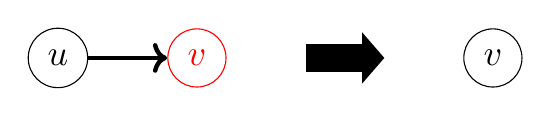
\begin{tikzpicture}[scale=1.3, node/.style={draw,circle,scale=1.3}]
            \node[node] (u1) {$u$};
            \node[node, right = of u1, red] (v1) {$v$};
            \coordinate[right = of v1] (a);
            \coordinate[right = of a] (b);
            
            \node[node, right = of b] (u2) {$v$};
    
            \draw[->, ultra thick, black] (u1) -- (v1);
            \draw[-{Triangle[width=18pt,length=8pt]}, line width=10pt] (a) -- (b);
        \end{tikzpicture}
    \end{figure}

    \item \textit{\textbf{RII}} --- remoção de vértices de grau dois, após os custos serem contabilizados na matriz de custos da nova aresta entre os dois vizinhos. Se necessário, a aresta é criada primeiro;

    \begin{figure}[H]
        \centering
        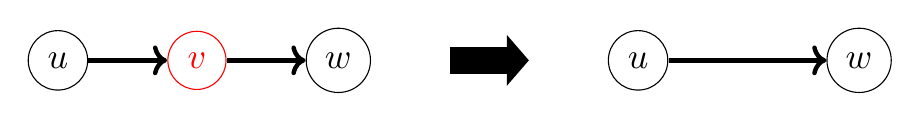
\begin{tikzpicture}[scale=1.3, node/.style={draw,circle,scale=1.3}]
            \node[node] (u1) {$u$};
            \node[node, right = of u1, red] (v1) {$v$};
            \node[node, right = of v1] (w1) {$w$};
            \draw[->, ultra thick, black] (u1) -- (v1);
            \draw[->, ultra thick, black] (v1) -- (w1);
            
            \coordinate[right = of w1] (a);
            \coordinate[right = of a] (b);

            \node[node, right = of b] (u2) {$u$};
            \coordinate[right = of u2] (c);
            \node[node, right = of c] (w2) {$w$};
            \draw[->, ultra thick, black] (u2) -- (w2);
            
            \draw[-{Triangle[width=18pt,length=8pt]}, line width=10pt] (a) -- (b);
        \end{tikzpicture}
    \end{figure}

    \item \textit{\textbf{RN}} --- remoção de vértices de grau três ou maior. Dado um vértice $u$, é escolhido um mínimo local e os custos de $u$ são distribuídos entre seus vizinhos. Em seguida, $u$ é removido e as arestas são removidas usando \textit{RE}.

    \begin{figure}[H]
        \centering
        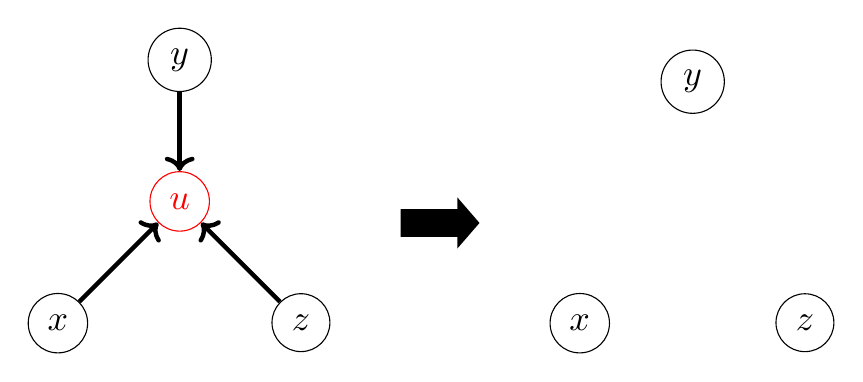
\begin{tikzpicture}[scale=1.3, node/.style={draw,circle,scale=1.3}]
            \node[node, red] (u) {$u$};
            \node[node, above = of u] (y1) {$y$};
            \node[node, below left = of u] (x1) {$x$};
            \node[node, below right = of u] (z1) {$z$};
            \draw[->, ultra thick, black] (x1) -- (u);
            \draw[->, ultra thick, black] (y1) -- (u);
            \draw[->, ultra thick, black] (z1) -- (u);
            
            \coordinate[above right = of z1] (a);
            \coordinate[right = of a] (b);
            \node[node, below right = of b] (x2) {$x$};
            \node[node, above right = of x2, white] (u2) {};

            \node[node, above = of u2] (y2) {$y$};
            \node[node, below right = of u2] (z2) {$z$};
            
            \draw[-{Triangle[width=18pt,length=8pt]}, line width=10pt] (a) -- (b);
        \end{tikzpicture}
    \end{figure}
\end{enumerate}

As reduções \textit{RE}, \textit{RI}, e \textit{RII} produzem subdivisões da instância original de igual custo mínimo, permitindo estender a seleção dos problemas menores para o problema original sem comprometer a qualidade da solução. Se o grafo inteiro puder ser reduzido dessa maneira, então é possível encontrar uma solução ótima para dada instância do problema. Se \textit{RN} for aplicada, no entanto, as subpartes produzidas perdem a precisão de representação do problema e a solução final obtida torna-se quase-ótima, onde a proximidade de uma hipotética solução ótima é garantida através da heurística de escolha do mínimo local como alternativa.

Hames e Scholz \cite{hames:06} propuseram, em 2006, uma heurística alternativa para a redução \textit{RN} que elimina a escolha de uma alternativa na etapa de redução, efetivamente a postergando para a fase de retropropagação das soluções. Além disso, eles introduziram um abordagem \textit{branch-and-bound} que consiste em utilizar de um limiar para dividir as possíveis combinações de escolhas, de tal modo que as combinações que certamente não são ótimas são descartadas e nunca são avaliadas pelo alocador. Essas heurísticas garantem resolução em tempo linear, e as reduções tornam a alocação via PBQP especialmente poderosa em instâncias que produzem grafos de interferência esparsos, pois permitem a alocação de maneira trivial.

\chapter{Minimização de \textit{Spill Code}}

Mesmo com a utilização de algoritmos refinados de alocação, em vários casos a introdução de \textit{spill code} no código resultante é factualmente inevitável. Sendo assim, um bom alocador deve produzir uma alocação visando minimizar o tráfego de dados entre a memória principal e o processador, devido ao grande atraso provocado pela execução de instruções de acesso à memória. Essas operações são responsáveis pela maior parte do gasto energético em sistemas computacionais \cite{verma:06}, e a alocação de registradores pode impactar o tempo de execução de um programa em até 250\% \cite{pereira:08}.

Dentre os problemas enfrentados pelos desenvolvedores de compiladores, há a notável tarefa de se decidir qual registrador virtual será enviado para a memória. A escolha deve ser tomada de modo a reduzir a pressão de registradores nos pontos problemáticos do código, preferencialmente tornando-o inteiramente alocável e resolvendo o problema com o \textit{spill} de uma única variável. No entanto, a escolha de uma variável frequentemente acessada, que está dentro de um laço de repetição ou é usada como controle, pode acidentalmente produzir muito mais acessos à memória no programa \cite{chaitin:82, bernstein:89}.

Além disso, há espaço para diferentes análises na tarefa de se estimar custos de \textit{spill}. Diferentes métodos de se definir o custo das operações de acesso à memória e calcular o custo associado à escolha de cada variável são possíveis, e podem produzir resultados diferentes considerando a especificidade arquitetura-alvo. Sendo assim, os desenvolvedores de compiladores dependem de experimentação e ``tentativa e erro'' para ajustar suas heurísticas de alocação \cite{amarasinghe:03}.

\section{Heurísticas de Chaitin}

A proposta inicial do primeiro alocador via coloração de grafos, feita por Chaitin \textit{et al.} em 1981, não continha heurísticas significativas para otimizar a introdução de \textit{spill code}. Inicialmente, a prioridade de escolha para a realização de \textit{spill} era dada às variáveis denominadas \textit{pass-through} --- isto é, que estão vivas na entrada dos blocos básicos e não são usadas nem redefinidas posteriormente. Instruções de \texttt{store} eram inseridas após toda redefinição do \textit{live range} escolhido, e os \texttt{loads} eram necessários antes de qualquer uso \cite{chaitin:81}.

Sendo assim, em um trabalho posterior de 1982 \cite{chaitin:82}, Chaitin formalizou heurísticas para a tomada de decisões de \textit{spill} que almejavam reduzir a quantidade de acessos a memória em tempo de execução. O custo de \textit{spill} de um registrador virtual é definido como o aumento no tempo de execução caso ele resida em memória, que corresponde ao número de pontos de definição mais o número de usos do valor. Por suas vezes, as definições e usos são ponderados levando em conta suas frequências estimadas de execução.

O custo de \textit{spill} associado a um \textit{live range} $v$ no alocador de Chaitin é dado pela Fórmula \ref{chaitin-custo}, onde $i$ é uma instrução contida no conjunto de instruções da IR do programa $I$, que manipula $v$ através de um uso ou uma redefinição, representados respectivamente pelos predicados $\mathit{use}_v(i)$ e $\mathit{def}_v(i)$. A função $\mathit{profundidade} (i)$ expressa o nível de aninhamento de $i$ dentro de laços de repetição. 

\begin{equation}
    \textit{custo}(v) = \sum_{\mathclap{\substack{i \in I\\\textit{use}_v(i) \lor \textit{def}_v(i)}}} 10 ^ {\textit{profundidade}(i)}
    \label{chaitin-custo}
\end{equation}

Os custos são computados quando, durante a etapa de \textit{simplify}, não são encontrados mais vértices aptos a serem removidos do grafo de interferência e o algoritmo trava. Em seguida, o alocador define as prioridades para a escolha de qual variável sofrerá \textit{spill} utilizando a Fórmula \ref{chaitin-prioridade}. Para cada \textit{live range}, o custo é dividido pelo grau do vértice correspondente no grafo e o vértice com menor valor ponderado é escolhido para sofrer \textit{spill} em todo o código \cite{bernstein:89}.

\begin{equation}
    h(v) = \frac{\textit{custo}(v)}{\textit{grau}(v)}
    \label{chaitin-prioridade}
\end{equation}

Chaitin \cite{chaitin:82} ainda introduziu o conceito de proximidade entre instruções: duas instruções são ditas próximas se nenhum \textit{live range} for eliminado entre elas e, consequentemente, nenhum registrador for liberado para alocação nesse intervalo. Esse princípio fundamenta um conjunto de três diretrizes que buscam evitar a inserção de \textit{reloads} desnecessários no código. São elas:
\begin{enumerate}
    \item Se uma definição e um uso são próximos, não é necessário adicionar um \texttt{load} antes do uso. Isso ocorre porque, como não foram disponibilizados novos registradores entre as instruções, o registrador da segunda instrução está disponível para a primeira. Sendo assim, é possível alocar o mesmo registrador para as duas utilizações;
    \item Se duas instruções de uso são próximas, é necessário introduzir um \texttt{load} somente antes do primeiro uso. De maneira análoga à diretriz anterior, o mesmo registrador pode ser reaproveitado na segunda instrução;
    \item Se a primeira definição e o último uso de um \textit{live range} são próximos, então o custo de \textit{spill} do registrador virtual é considerado infinito. Como nenhum registrador é liberado, enviar a variável para memória não tornará o programa colorível.
\end{enumerate}
    
\section{Heurísticas de Bernstein}

Em um trabalho de 1989, Bernstein \textit{et al.} \cite{bernstein:89} pontuaram uma série de problemas com o alocador de Chaitin. Em primeiro lugar, a heurística empregada na decisão de \textit{spill} pode não ser a mais eficiente em todas as instâncias de alocação. Além disso, o alocador de Chaitin insere instruções \texttt{store}/\texttt{load} desnecessariamente em todos os pontos do antigo \textit{live range}, sendo que elas podem somente ser necessárias em pontos de grande pressão de registradores. 

Sendo assim, o trabalho trouxe algumas técnicas e novas heurísticas visando expandir as contribuições de Chaitin. Essas melhorias se mostraram capazes de reduzir a quantidade de código \textit{spill}, na média, em 6\% e 12\%, chegando até 30\% em alguns casos.

\subsection{\textit{Best-of-three}}

Bernstein \textit{et al.} notaram que, a respeito da heurística de decisão de \textit{spill}, não se pode fazer uma afirmação absoluta sobre o desempenho de uma função heurística simples em relação a outra para todos os programas. Ao contrário, diferentes instâncias de problemas de alocação podem exigir estratégias distintas para a obtenção de melhores resultados. Eles propuseram comparar o desempenho médio de diferentes fórmulas, mantendo em mãos um seleto número funções heurísticas que vislumbrem as diferentes causas da pressão de registradores, e escolhendo a melhor delas para tomar as decisões de \textit{spill}.

A heurística $h_1$ (Fórmula \ref{eq:bernstein-1}) tem em vista a estratégia original de Chaitin, que consiste em escolher um vértice com baixo custo e alto grau. Realizar \textit{spill} de uma variável com alto grau reduz o grau de muitos outros vértices no grafo de interferência, tornando mais provável que outros vértices se tornem desobstruídos.

\begin{equation}
    h_1(v) = \frac{\textit{custo}(v)}{\textit{grau}(v)^2}
    \label{eq:bernstein-1}
\end{equation}

Alternativamente, a abordagem escolhida pode ser a de se fazer \textit{spill} do registrador virtual que exerça a maior pressão de registradores sobre o código. Sendo assim, é introduzido o conceito de área de uma variável, computado através da Fórmula \ref{bernstein-area}:
\begin{equation}
    \textit{área}(v) = \sum_{\mathclap{\substack{i \in I\\v\text{ vivo em }i}}} 5 ^ {\textit{profundidade}(i)} \textit{largura}(i)
    \label{bernstein-area}
\end{equation}
onde $\mathit{largura}(i)$ é o número de variáveis vivas no momento de execução da instrução $i$. De maneira intuitiva, $\textit{área}(v)$ expressa o impacto de $v$ para a pressão de registradores global. A escolha de uma variável com alta área causa uma redução considerável na pressão em todo o programa, e facilita a coloração. As heurísticas seguintes $h_2$ e $h_3$ (Fórmulas \ref{eq:bernstein-2} e \ref{eq:bernstein-3}) se fundamentam nesse princípio.

\begin{equation}
    h_2(v) = \frac{\mathit{custo}(v)}
                  {\textit{área}(v)\mathit{grau}(v)}
    \label{eq:bernstein-2}
\end{equation}

\begin{equation}
    h_3(v) = \frac{\mathit{custo}(v)}
                  {\textit{área}(v) \mathit{grau}(v) ^ 2}
    \label{eq:bernstein-3}
\end{equation}

O algoritmo proposto por Bernstein \textit{et al.} efetua efetua a coloração do grafo de interferência múltiplas vezes, para cada heurística $h_i$ disponível. O resultado final escolhido é o da heurística que produza o menor custo total de \textit{spill}. Essa técnica, apelidada de ``\textit{best-of-three}'', superou as abordagens anteriores consideravelmente, sob penalidade de um tempo de compilação ligeiramente maior.

\subsection{\textit{Coloração Gulosa}}

Bernstein \textit{et al.} \cite{bernstein:89} também introduziram heurísticas de coloração que se baseiam em adotar uma estratégia local para cada região do programa. É sabido que o grafo de interferência pode conter diversos subgrafos com diferentes características, sendo que alguns deles podem ser coloridos em tempo polinomial \cite{golumbic:04, dagan:88}. Dessa maneira, diferentes formas de coloração podem ser adotadas em diferentes porções do código, e os resultados combinados para compor a alocação final.

O algoritmo de coloração de por Bernstein \textit{et al.} realiza a etapa de \textit{simplify} removendo sempre o vértice apto de maior grau. Logo, na etapa de \textit{select}, os registradores são alocados em ordem crescente de grau para cada \textit{live range}. Ademais, após a $k$-colorabilidade do grafo de interferência ter sido assegurada, um critério secundário pode usado para colori-lo com, geralmente, menos cores do que em uma atribuição aleatória. Em certas situações, isso pode melhorar o código resultante, como:

\begin{itemize}
    \item A alocação produziu \textit{spills} a mais, e torna-se possível colorir o grafo com menos do que $k$ cores. Nesse caso, as $k - n$ decisões de \textit{spill} mais custosas da iteração anterior podem ser desfeitas;
    \item Pequenos procedimentos chamados frequentemente, onde uma utilização de registradores econômica pode reduzir o \textit{overhead} das chamadas;
    \item Expansões \textit{inline} de funções, onde a decisão de expandir ou não é influenciada pela quantidade de registradores utilizados na sub-rotina.
\end{itemize}

\subsection{\textit{Cleaning}}

Bernstein \textit{et al.} \cite{bernstein:89} resolveram o problema da inserção desnecessária de instruções \texttt{store}/\texttt{load} através da técnica denominada pelos autores como ``\textit{cleaning}'', ou limpeza. Esse método consiste em, quando uma variável for enviada para a memória, inserir somente uma instrução \texttt{store} e um \texttt{load} por bloco básico. Ao examinar um bloco em busca de valores que sofreram \textit{spill}, os acessos à memória são introduzidos apenas no primeiro uso ou definição do \textit{live range}. Em seguida, a variável é renomeada em cada bloco básico em que é usada, fragmentando o tempo de vida original.

Os autores observaram que o \textit{cleaning} é bem sucedido em reduzir o número total de instruções de acesso à memória, especialmente nas primeiras duas iterações de coloração/\textit{spill}, e quando nenhuma restrição é imposta à profundidade dos blocos básicos nos quais a limpeza é realizada ou aos registradores para os quais a limpeza é aplicada. O pseudocódigo mostrando o fluxo de execução da técnica de Bernstein \textit{et al.} com a realização do \textit{cleaning} encontra-se no Algoritmo \ref{alg:bernstein}.

\begin{algoritmo}[hb]
    \caption{Algoritmo de coloração utilizando \textit{best-of-three}. Extraído de Bernstein \textit{et al.} \cite{bernstein:89}}
    \begin{algorithmic}
        \Require $R$: conjunto de registradores físicos, $G$: grafo de interferência, $S_i$: lista de \textit{spill} associada à heurística $h_i$, $h_i$: heurística.
        \Procedure{ColorAndSpill}{}
            \ForAll{método heurístico $h_i$}
                \While{$G$ não é vazio}{}
                    \If{existe um $v$ no grafo $G$ tal que $\mathit{grau}(v) < |R|$}
                        \State escolha o $v$ com maior grau (tal que $\mathit{grau}(v) < |R|$)
                        \State $G \gets G - \{v\}$
                    \Else
                        \State escolha um $v$ tal que $\text{min }h_i(v)$
                        \State $S_i \gets S_i \cup \{v\}$
                        \State $G \gets G - \{v\}$
                    \EndIf
                \EndWhile
                \State restaure $G$
            \EndFor

            \State escolha a heurística $h_i$ com o menor $\mathit{custo}(S_i)$
            \If{nenhum vértice tiver sofrido \textit{spill}}
                \State pinte os vértices em ordem reversa da remoção de $G$
            \Else
                \ForAll{vértice $v \in S_i$}
                    \Call{Spill}{v}
                \EndFor
                \State realize \textit{``cleaning''} nos blocos básicos
                \State reconstrua o grafo $G$
            \EndIf
        \EndProcedure
    \end{algorithmic}
    \label{alg:bernstein}
\end{algoritmo}

\section{\textit{Spilling} por Região de Interferência}

Em 1997, Bergner \textit{et al.} publicaram um artigo \cite{bergner:97} pontuando que as heurísticas prévias ainda produziam \textit{spill} code desnecessariamente, pois as instruções de acesso à memória eram inseridas ao longo de todo o tempo de vida que era escolhido para \textit{spill}. Em resposta a esse problema, Bergner \textit{et al.} introduziu o conceito de \textit{spilling} por região de interferência, que consistia em limitar as alterações no código somente às regiões de sobreposição entre os \textit{live ranges}, nos pontos de alta pressão de registradores.

Nessa abordagem, uma região de interferência entre dois registradores virtuais é dita como a porção do programa onde ambos estão vivos simultaneamente, e elas são diretamente representadas no grafo de interferência na forma das arestas. Em adição às técnicas de minimização de \textit{spill code} propostas por Chaitin \cite{chaitin:81}, Bernstein \cite{bernstein:89} e Briggs \cite{briggs2:92}, o alocador de Bergner limita a introdução de \textit{reloads} somente aos usos da variável dentro da região de interferência. No caso em que o \textit{live range} é utilizado novamente após a região de interferência, deve-se introduzir um \textit{reload} adicional para recarregar o valor de volta para um registrador físico.

\begin{figure}[hbt]
    \centering
    \adjustbox{center}{\begin{lstlisting}
A = input();
B = A + 1;
if (A) {
    C = A + 2;
    B = A + C;
    if (C) {
        B = B + C;
        C = B + C;
    }
    A = B + C;
}
D = A + B;
    \end{lstlisting}}
    \caption{Exemplo de programa em pseudocódigo extraído de Bergner \textit{et al.} \cite{bergner:97}.}
    \label{fig:bergner-codigo}
\end{figure}

\begin{figure}[hbt]
        \centering
        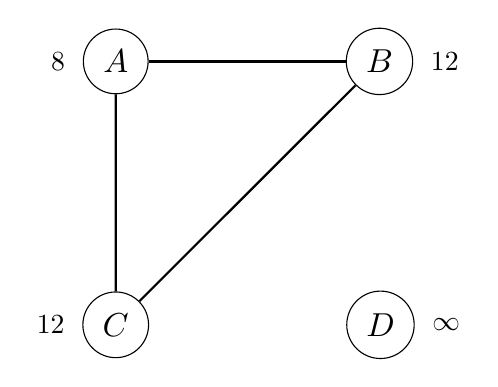
\begin{tikzpicture}[scale=2, node/.style={draw,circle, scale=1.2}]
            \node[node] (A) {$A$};
            \node[left = 1mm of A] {$8$};
            \node[node, right = 25mm of A] (B) {$B$};
            \node[right = 1mm of B] {$12$};
            \node[node, below = 25mm of A] (C) {$C$};
            \node[left = 1mm of C] {$12$};
            \node[node, right = 25mm of C] (D) {$D$};
            \node[right = 1mm of D] {$\infty$};

            \draw[black, thick] (A) -- (B);
            \draw[black, thick] (A) -- (C);
            \draw[black, thick] (C) -- (B);
        \end{tikzpicture}
        \caption{Grafo de interferência correspondente ao código da Figura \ref{fig:bergner-codigo}, com os custos de \textit{spill} indicados.}
        \label{fig:bergner-grafo}
    \end{figure}

Para escolher quais regiões de interferência sofrerão \textit{spill}, a estratégia desenvolvida por Bergner é aplicada durante a etapa de \textit{select} de um alocador ao estilo de Briggs, durante a reintrodução dos vértices no grafo e concomitante alocação de cores. Ao se tentar reintroduzir um vértice $v$ candidato a \textit{spill} --- o que não será inteiramente possível devido ao número de interferências de $v$, suas arestas são agrupadas em conjuntos, cada conjunto contendo as arestas que se conectam a vértices de uma mesma cor. O alocador deve então tentar colorir $v$, não inserindo no grafo as arestas do conjunto cuja cor já está atribuída a algum dos seus vizinhos. 

O custo de se fazer \textit{spill} de $v$ em cada região de interferência é calculado levando em conta a quantidade estimada de instruções \texttt{store}/\texttt{load} que serão introduzidas no código, e a cor selecionada para o vértice candidato deve ser a que minimize o total desse custo. Uma vez que a cor é definida, as regiões de interferência cujas arestas correspondentes não puderam ser inseridas no grafo são escolhidas para sofrerem \textit{spill}. A Figura \ref{fig:bergner-grafo-col} demonstra esse processo ao tentar colorir o grafo da Figura \ref{fig:bergner-grafo}, onde o vértice candidato $A$ recebe a mesma cor de $C$, impedindo que a aresta $AC$ seja introduzida no grafo. Ela é então descartada, e $A$ sofrerá \textit{spill} na região de interferência entre $A$ e $C$.

\begin{figure}[hbt]
    \centering
    \begin{subfigure}{0.44\textwidth}
        \centering
        \adjustbox{valign=c}{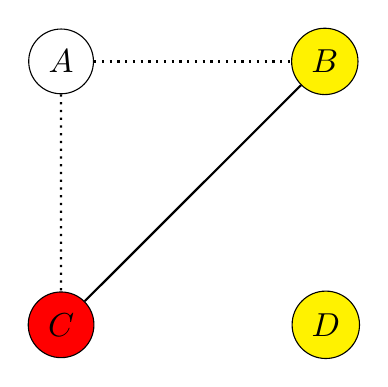
\begin{tikzpicture}[scale=2, node/.style={draw,circle, scale=1.2}]
            \node[node] (A) {$A$};
            \node[node, right = 25mm of A, fill=yellow] (B) {$B$};
            \node[node, below = 25mm of A, fill=red] (C) {$C$};
            \node[node, right = 25mm of C, fill=yellow] (D) {$D$};

            \draw[black, thick, dotted] (A) -- (B);
            \draw[black, thick, dotted] (A) -- (C);
            \draw[black, thick] (C) -- (B);
        \end{tikzpicture}}
    \end{subfigure}
    \begin{subfigure}{0.1\textwidth}
        \centering
        \adjustbox{valign=c}{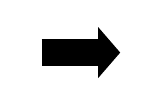
\begin{tikzpicture}
            \draw[-{Triangle[width=18pt,length=8pt]}, line width=10pt] (0,5) -- (1,5);
        \end{tikzpicture}}
    \end{subfigure}
    \begin{subfigure}{0.44\textwidth}
        \centering
        \adjustbox{valign=c}{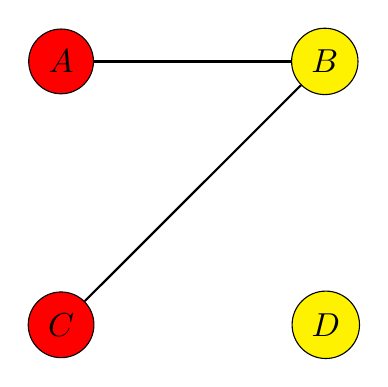
\begin{tikzpicture}[scale=2, node/.style={draw,circle, scale=1.2}]
            \node[node, fill=red] (A) {$A$};
            \node[node, right = 25mm of A, fill=yellow] (B) {$B$};
            \node[node, below = 25mm of A, fill=red] (C) {$C$};
            \node[node, right = 25mm of C, fill=yellow] (D) {$D$};

            \draw[black, thick] (A) -- (B);
            \draw[black, thick] (C) -- (B);
        \end{tikzpicture}}
    \end{subfigure}
    \caption{Coloração do exemplo da Figura \ref{fig:bergner-grafo}, considerando a estratégia de \textit{spilling} por região de interferência. Adaptado de Bergner \textit{et al.} \cite{bergner:97}.}
    \label{fig:bergner-grafo-col}
\end{figure}

A comparação entre o código gerado pela técnica tradicional e o pelo \textit{spilling} por região de interferência é exibida na Figura \ref{fig:bergner-comparacao}. A estratégia de Bergner \textit{et al.} apresentou altas taxas de sucesso em experimentos, conquistando uma redução média de 33,6\% no número de instruções de acesso a memória executadas dinamicamente, atingindo a faixa de 75\% em alguns casos \cite{bergner:97}. Essa técnica superou de longe as heurísticas anteriores, e representou um avanço significativo na minimização de \textit{spill code}. 

\begin{figure}[H]
    \centering
    \begin{subfigure}{0.49\textwidth}
        \centering
        \adjustbox{center}{\begin{lstlisting}[mathescape=true]
A = input();
store A;
B = A + 1;
if (A) {
    load $\texttt{A}_1$;
    C = $\texttt{A}_1$ + 2;
    B = $\texttt{A}_1$ + C;
    if (C) {
        B = B + C;
        C = B + C;
    }
    $\texttt{A}_2$ = B + C;
    store $\texttt{A}_2$;
}
load $\texttt{A}_3$;
D = A + B;
        \end{lstlisting}}
    \end{subfigure}
    \begin{subfigure}{0.49\textwidth}
        \centering
        \adjustbox{center}{\begin{lstlisting}[mathescape=true]
A = input();
store A;
B = A + 1;
if (A) {
    load $\texttt{A}_1$;
    C = $\texttt{A}_1$ + 2;
    B = $\texttt{A}_1$ + C;
    if (C) {
        B = B + C;
        C = B + C;
    }
    A = B + C;
    
}

D = A + B;
        \end{lstlisting}}
    \end{subfigure}
    \caption{Comparação entre os resultados da técnica tradicional e do \textit{spilling} por região de interferência. Na esquerda, \texttt{A} sofre \textit{spill} em todo o código, enquanto na direita a inserção de \textit{spill code} ocorre somente na interferência entre \texttt{A} e \texttt{C}. Adaptado de Bergner \textit{et al.} \cite{bergner:97}.}
    \label{fig:bergner-comparacao}
\end{figure}

\section{Rematerialização}

Em seu trabalho de 1982, Chaitin \textit{et al.} \cite{chaitin:82} já haviam demonstrado que é preferível inserir instruções para recalcular certos valores ao invés de armazená-los em memória, devido ao custo mais baixo de fazê-lo. Essa técnica foi denominada ``\textit{rematerialization}'', ou rematerialização, e representa uma alternativa à geração de \textit{spill code} em situações onde a pressão de registradores ultrapassa o número de registradores físicos disponíveis. Posteriormente, Briggs \textit{et al.} \cite{briggs2:92} refinaram essa técnica, introduzindo novos conceitos e propondo uma metodologia que permite uma otimização mais profunda.

Chaitin \textit{et al.} mostraram que certos valores podem ser recalculados com uma única instrução adicional, caso os operandos necessários estejam sempre disponíveis. Eles denominaram esses casos excepcionais como valores \textit{``never-killed''}, e argumentaram que é mais barato recomputar tais valores do que armazená-los e constantemente acessar a memória para recuperá-los. Na prática, boas oportunidades para a rematerialização incluem \texttt{loads} imediatos de constantes e o cálculo de endereços de memória, com ou sem \textit{offset}. Entretanto, o alocador de Chaitin só pode rematerializar \textit{live ranges} que assumem um único valor ao longo de toda sua extensão, não sendo capaz de lidar com casos mais complexos.

Sendo assim, em 1992 Briggs \textit{et al.} \cite{briggs2:92} expandiram a técnica de Chaitin para tratar \textit{live ranges} multivalorados. Sua abordagem consistia em dividir os tempos de vida para cada valor que assumem ao longo da execução de um programa, efetivamente convertendo a representação intermediária para a forma SSA (\textit{static single-assignment}). Na forma SSA, cada variável é definida uma única vez antes de ser obrigatoriamente usada, e por isso possui apenas um valor ao longo do seu tempo de vida. 

No processo de conversão para a forma SSA, os \textit{live ranges} dão origem vários tempos de vida menores definidos uma única vez, a partir de um valor simples ou uma função-$\phi$ --- artifício que representa a utilização de um dentre múltiplos valores possíveis em tempo de execução. A Figura \ref{fig:ssa} apresenta um exemplo de código nas formas tradicional e SSA, onde a variável \texttt{w} é definida a partir de \texttt{y}, que recebe valores diferentes em cada caso de uma ramificação condicional. Sendo assim, deve ser criada uma nova variável $\texttt{y}_3$ que pode receber tanto o valor de $\texttt{y}_1$ quanto $\texttt{y}_2$, a depender de qual bloco condicional será acessado em tempo de execução.

\begin{figure}[hbt]
    \centering
    \begin{subfigure}{0.40\textwidth}
        \centering
        \adjustbox{valign=c}{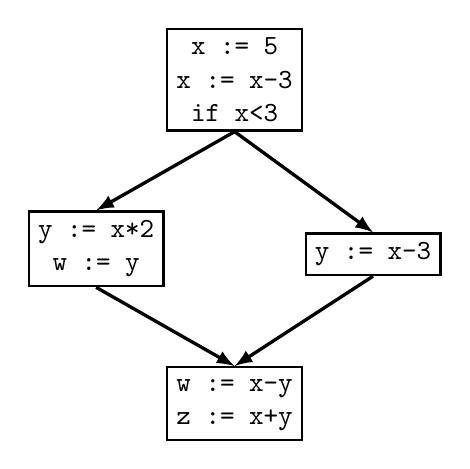
\begin{tikzpicture}[CFG/.style={rectangle, draw=black!100, fill=white!100, thick, minimum size=5mm, align=center}]

            \node[CFG] (B0) {\texttt{x := 5}\\
                             \texttt{x := x-3}\\
                             \texttt{if x<3}};
    
            \node[CFG, below right = 12.8mm and 0.2mm of B0] (B1) 
                {\texttt{y := x-3}};
            \node[CFG, below left = 10mm and 0.2mm of B0] (B2) 
                {\texttt{y := x*2}\\
                 \texttt{w := y}};
            \node[CFG, below right = 10mm and 0.2mm of B2] (B3) 
                {\texttt{w := x-y}\\
                 \texttt{z := x+y}};

            \draw[-latex, black, very thick] (B0.south) -- (B1.north) {};
            \draw[-latex, black, very thick] (B0.south) -- (B2.north) {};
            \draw[-latex, black, very thick] (B1.south) -- (B3.north) {};
            \draw[-latex, black, very thick] (B2.south) -- (B3.north) {};
        \end{tikzpicture}}
    \end{subfigure}
    \begin{subfigure}{0.09\textwidth}
        \centering
        \adjustbox{valign=c}{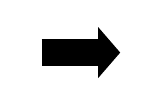
\begin{tikzpicture}
            \draw[-{Triangle[width=18pt,length=8pt]}, line width=10pt] (0,5) -- (1,5);
        \end{tikzpicture}}
    \end{subfigure}
    \begin{subfigure}{0.40\textwidth}
        \centering
        \adjustbox{valign=c}{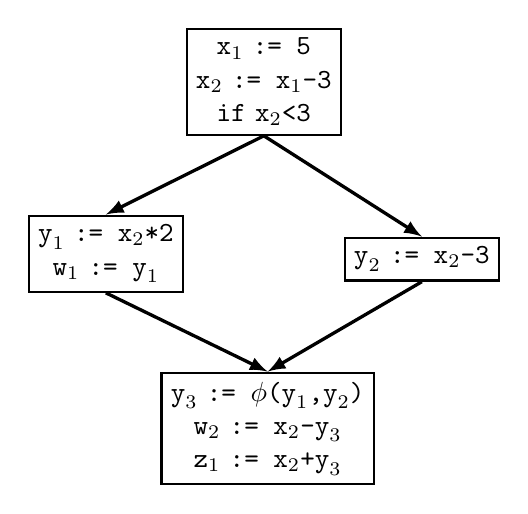
\begin{tikzpicture}[CFG/.style={rectangle, draw=black!100, fill=white!100, thick, minimum size=5mm, align=center}]

            \node[CFG] (B0) {$\texttt{x}_1\ \texttt{:= 5}$\\
                             $\texttt{x}_2\ \texttt{:= x}_1\texttt{-3}$\\
                             \texttt{if} $\texttt{x}_2\texttt{<3}$};
    
            \node[CFG, below right = 12.8mm and 0.2mm of B0] (B1) 
                {$\texttt{y}_2\ \texttt{:= x}_2\texttt{-3}$};
            \node[CFG, below left = 10mm and 0.2mm of B0] (B2) 
                {$\texttt{y}_1\ \texttt{:= x}_2\texttt{*2}$\\
                 $\texttt{w}_1\ \texttt{:= y}_1$};
            \node[CFG, below right = 10mm and -0.3 of B2] (B3) 
                {$\texttt{y}_3\ \texttt{:= }\phi\texttt{(y}_1\texttt{,y}_2\texttt{)}$\\
                 $\texttt{w}_2\ \texttt{:= x}_2\texttt{-y}_3$\\
                 $\texttt{z}_1\ \texttt{:= x}_2\texttt{+y}_3$};

            \draw[-latex, black, very thick] (B0.south) -- (B1.north) {};
            \draw[-latex, black, very thick] (B0.south) -- (B2.north) {};
            \draw[-latex, black, very thick] (B1.south) -- (B3.north) {};
            \draw[-latex, black, very thick] (B2.south) -- (B3.north) {};
        \end{tikzpicture}}
    \end{subfigure}
    \caption{Exemplo de código na forma tradicional e após a conversão para forma SSA.}
    \label{fig:ssa}
\end{figure}

Em seguida, as instruções de definição dos valores são rotuladas como candidatas ou não à rematerialização. Para isso, Briggs \textit{et al.} empregaram um algoritmo semelhante ao \textit{constant propagation} de Wegman e Zadeck \cite{wegman:91}, para propagar as rotulações pelo grafo de controle de fluxo. Os rótulos consistem de:
\begin{itemize}
    \item $\top$ --- significa que nenhuma informação é conhecida. Um valor definido por uma instrução de cópia ou uma função-$\phi$ recebem este rótulo de imediato;
    \item \textit{inst} --- valor definido por uma instrução adequada (\textit{never-killed}. Na implementação é um ponteiro para a própria instrução;
    \item $\bot$ --- valor que deve sofrer \textit{spill}. Valores inapropriados para a rematerialização recebem este rótulo de imediato.
\end{itemize}

Quando o rótulo de uma variável é propagado para as instruções que a utilizam ocorre uma operação de \textit{``meeting''}, ou encontro, denotada pelo símbolo $\sqcap$. Ela é efetuada entre rótulos, e é definida matematicamente através das Fórmulas \ref{eq:meet-1}, \ref{eq:meet-2} e \ref{eq:meet-3}:
\begin{equation}
    x \sqcap \top = x
    \label{eq:meet-1}
\end{equation}
\begin{equation}
    x \sqcap \bot = \bot
    \label{eq:meet-2}
\end{equation}
\begin{equation}
    \mathit{inst}_i \sqcap \mathit{inst}_j = 
    \begin{cases}
        \mathit{inst}_i, & \text{se } \mathit{inst}_i = \mathit{inst}_j \\
        \bot, & \text{se } \mathit{inst}_i \ne \mathit{inst}_j
    \end{cases}
    \label{eq:meet-3}
\end{equation}
onde $x$ é qualquer rótulo, e a comparação $\mathit{inst}_i = \textit{inst}_j$ é realizada operando a operando. Os valores são todos inicializados como $\top$, e durante a propagação valores definidos por uma instrução de cópia terão seus rótulos reduzidos para \textit{inst} ou $\bot$. Valores definidos por funções-$\phi$ serão reduzidos para \textit{inst} se e somente se todos os valores o atingindo tiverem rótulos equivalentes; caso contrário, eles recebem $\bot$.

Concluída a propagação, os nós-$\phi$ devem ser removidos e os valores renomeados para que o programa executável seja produzido. Valores rotulados como \textit{never-killed} são rematerializados no código final e possíveis divisões desnecessárias dos \textit{live ranges}, remanescentes da forma SSA, são removidas através de processos presentes em um alocador estilo Briggs \cite{briggs:92}, como coalescimento e coloração com a mesma cor de variáveis unidas por cópia.

O algoritmo de Briggs \textit{et al.} foi testado em 70 benchmarks e apresentou uma redução considerável de \textit{spill code} em 28 dos casos, com melhorias que ultrapassaram os 20\%. Os autores também observaram uma redução nas instruções de \texttt{store}, \texttt{load} e de cópia, o que indica que as heurísticas de remoção de divisões desnecessárias são adequadas \cite{briggs2:92}.

\section{Coloração de Grafos Hierárquica}

Em 1991, Callahan e Koblenz \cite{callahan:91} descreveram uma técnica de alocação de registradores que emprega uma heurística hierárquica de coloração de grafos, onde o programa é particionado em uma série de porções que constituem uma estrutura de árvore e que refletem a estrutura de controle do código. Então, para cada porção é realizada a coloração de grafos de maneira local, resultando numa alocação sensível aos padrões de utilização das variáveis em cada região do programa.

O princípio da abordagem de Callahan e Koblenz consiste em representar o fluxo de repetição e ramificação nos blocos básicos na forma de \textit{``tiles''}, que na prática constituem subárvores. Sendo o grafo de controle de fluxo (CFG) representado pela tupla $G = (B, E, \textit{start}, \textit{stop})$, onde $B$ é o conjunto dos blocos básicos, $E$ é o conjunto de arestas entre os blocos e $\mathit{start}, \textit{stop} \in B$ representam respectivamente os pontos de início e fim do fluxo de execução, é definida uma árvore hierárquica $T$.

Cada nó $t \in T$ é um membro da família de subconjuntos de $B$ tal que $\mathit{blocos}(t) = \{b_0, b_1, \dots, b_n\}$ e $\mathit{arestas}(t)=\{e_0, e_1, \dots, e_n\}$, onde $b$ são os blocos básicos pertencentes a $t$, mas que não pertencem a nenhuma subárvore de $t$, e $e$ são as arestas dos blocos em $\mathit{blocos}(t)$. Cada par de elementos em $t_1, t_2 \in T$ é ou disjunto, ou $t_1$ é subconjunto próprio de $t_2$ e não há nenhum outro $t$ tal que $t_1 \subset t \subset t_2$; nesse caso, dizemos que $t_1$ é nó-filho de $t_2$ e $t_2$ é nó-pai de $t_1$. Há também em todo programa uma raiz $t_0$ tal que $\mathit{blocos}(t_0) = \{\mathit{start}, \mathit{stop}\}$. A adição de novos nós na árvore do programa ocorre nas ramificações criadas por estruturas condicionais e em laços de repetição, como exemplificado na Figura \ref{arvore-programa}.

\begin{figure}[ht]
    \centering
    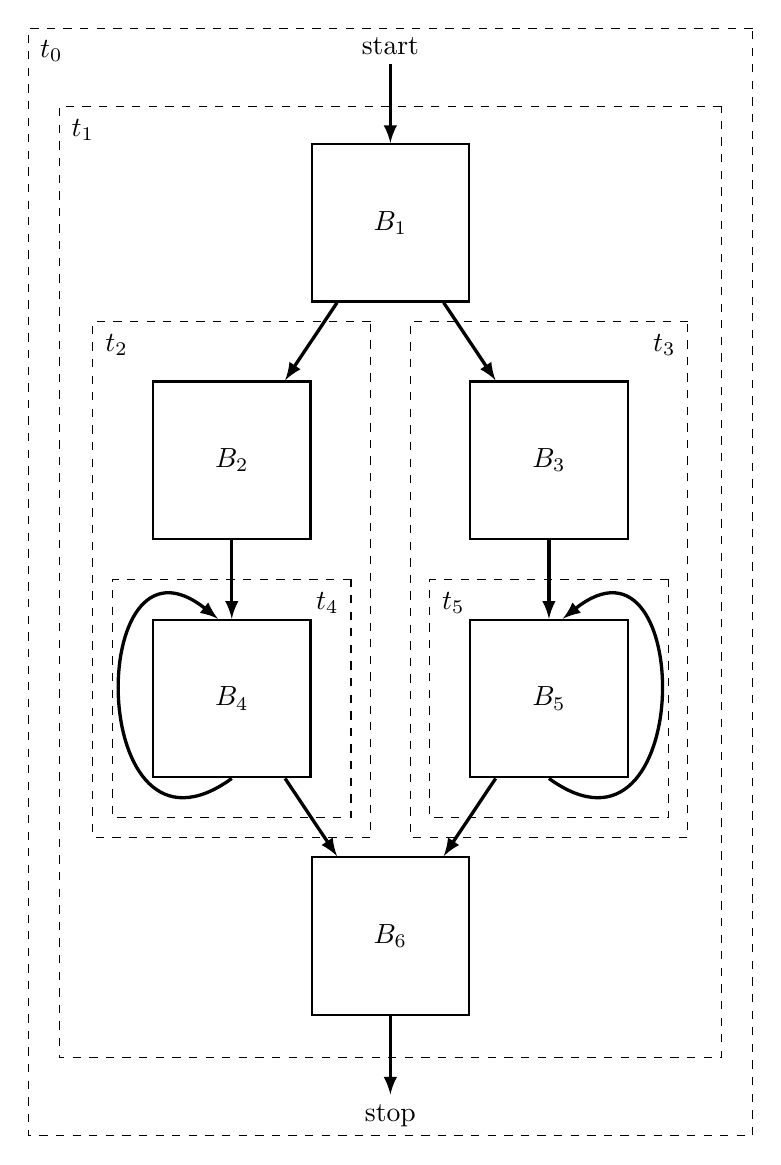
\begin{tikzpicture}[CFG/.style={rectangle, draw=black!100, fill=white!100, thick, minimum size=20mm, align=center}]
        \node (start) {start};
        \node[CFG, below = of start] (B1) {$B_1$};
        \coordinate[below = 20mm of B1] (C1);
        \node[CFG, left = of C1] (B2) {$B_2$};
        \node[CFG, right = of C1] (B3) {$B_3$};
        \node[CFG, below = of B2] (B4) {$B_4$};
        \node[CFG, below = of B3] (B5) {$B_5$};
        \coordinate[right = of B4] (C2);
        \node[CFG, below = 20mm of C2] (B6) {$B_6$};
        \node[below = of B6] (stop) {stop};

        \draw[-latex, very thick] (start) -- (B1);
        \draw[-latex, very thick] (B1) -- (B2);
        \draw[-latex, very thick] (B1) -- (B3);
        \draw[-latex, very thick] (B2) -- (B4);
        \draw[-latex, very thick] (B3) -- (B5);
        \draw[-latex, very thick] (B4) -- (B6);
        \draw[-latex, very thick] (B5) -- (B6);
        \draw[-latex, very thick] (B6) -- (stop);

        \coordinate[below left = 13.5mm and 8.5mm of B4] (E1);
        \coordinate[above left = 13.5mm and 8.5mm of B4] (E2);

        \coordinate[below right = 13.5mm and 8.5mm of B5] (E3);
        \coordinate[above right = 13.5mm and 8.5mm of B5] (E4);
        
        \draw[-latex, very thick] (B4.south) .. controls (E1) and (E2) .. ([xshift=-5] B4.north);
        \draw[-latex, very thick] (B5.south) .. controls (E3) and (E4) .. ([xshift=5] B5.north);

        \coordinate[below left = of B4] (F1);
        \coordinate[below right = of B4] (F2);
        \coordinate[above left = of B4] (F3);
        \coordinate[above right = of B4] (F4);

        \draw[dashed] ([xshift = 7mm] current bounding box.north east) -- ([xshift = -7mm] current bounding box.north west) -- ( current bounding box.south west) -- (current bounding box.south east) -- cycle;
        \node at ([xshift = 3mm, yshift = -3mm] current bounding box.north west) {$t_0$};

        \draw[dashed] ([xshift = -4mm, yshift = -10mm] current bounding box.north east) -- ([xshift = 4mm, yshift = -10mm] current bounding box.north west) -- ([xshift = 4mm, yshift = 10mm] current bounding box.south west) -- ([xshift = -4mm, yshift = 10mm] current bounding box.south east) -- cycle;
        \node at ([xshift = 7mm, yshift = -13mm] current bounding box.north west) {$t_1$};

        \draw[dashed] ([xshift = 7.5mm, yshift = 7.5mm] B2.north east) -- ([xshift = -7.5mm, yshift = 7.5mm] B2.north west) -- ([xshift = -7.5mm, yshift = -7.5mm] B4.south west) -- ([xshift = 7.5mm, yshift = -7.5mm] B4.south east) -- cycle;
        \node at ([xshift = -4.5mm, yshift = 4.5mm] B2.north west) {$t_2$};

        \draw[dashed] ([xshift = 7.5mm, yshift = 7.5mm] B3.north east) -- ([xshift = -7.5mm, yshift = 7.5mm] B3.north west) -- ([xshift = -7.5mm, yshift = -7.5mm] B5.south west) -- ([xshift = 7.5mm, yshift = -7.5mm] B5.south east) -- cycle;
        \node at ([xshift = 4.5mm, yshift = 4.5mm] B3.north east) {$t_3$};

        \draw[dashed] ([xshift = 5mm, yshift = 5mm] B4.north east) -- ([xshift = -5mm, yshift = 5mm] B4.north west) -- ([xshift = -5mm, yshift = -5mm] B4.south west) -- ([xshift = 5mm, yshift = -5mm] B4.south east) -- cycle;
        \node at ([xshift = 2mm, yshift = 2mm] B4.north east) {$t_4$};

        \draw[dashed] ([xshift = 5mm, yshift = 5mm] B5.north east) -- ([xshift = -5mm, yshift = 5mm] B5.north west) -- ([xshift = -5mm, yshift = -5mm] B5.south west) -- ([xshift = 5mm, yshift = -5mm] B5.south east) -- cycle;
        \node at ([xshift = -2mm, yshift = 2mm] B5.north west) {$t_5$};
    \end{tikzpicture}
    \caption{Exemplo de CFG particionado em porções correspondentes aos nós $t_0,t_1,\dots,t_5$ da árvore hierárquica.}
    \label{arvore-programa}
\end{figure}

Uma vez que a representação intermediária é organizada na forma da árvore hierárquica, a coloração de grafos é efetuada para cada nó de maneira recursiva em pós-ordem, ou \textit{``bottom-up''}. Para cada nó $t$, o grafo é montado contendo somente as variáveis cujo \textit{live range} é definido e usado inteiramente em $\mathit{blocos}(t)$, que são denominadas variáveis locais, e a coloração é feita de maneira convencional seguindo um algoritmo ao estilo de Briggs \cite{briggs:89}. Para todos os fins, as variáveis globais a $t$ --- isto é, que são definidas em níveis superiores da árvore e estão vivas na entrada dos blocos básicos de um nó --- são ignoradas, pois serão tratadas na alocação de algum nó ancestral de $t$. Uma vez concluída a coloração, as variáveis recebem registradores físicos diretamente ou pseudoregistradores, que funcionam como alcunhas para grupos de registradores da arquitetura-alvo. 

Ao retornar para a chamada anterior da recursão, o algoritmo prossegue para colorir o grafo do nó-pai $t_{pai}$ incluindo um conjunto de novas variáveis, cada uma delas sendo o coalescimento de todas as variáveis de $t$ que foram alocadas a um registrador distinto. Elas são denominadas ``variáveis de resumo'', e servem o propósito de indicar quais registradores já foram aproveitados na subárvore com raiz em $t$. Sendo assim, uma aresta é inserida no grafo de interferência de um nó se:
\begin{enumerate}
    \item Duas variáveis locais ao nó interferem em algum ponto de seus blocos;
    \item Uma variável global interfere com uma variável de resumo ou outra variável global;
    \item Uma variável está viva em uma subárvore de $t$ mas não consta nas variáveis de resumo vindas da subárvore;
    \item Uma variável de resumo conflita com outras variáveis de resumo da mesma subárvore.
\end{enumerate}

Uma vez que a raiz da árvore é colorida, a atribuição final de registradores  físicos ocorre de maneira \textit{``top-down''}, assim como a inserção de instruções de \textit{spill}. O \textit{spill code} é, de maneira geral, inserido nas entradas e saídas dos blocos básicos e consiste de instruções de acesso a memória para variáveis locais que sofreram \textit{spill} em um nó, instruções de cópia para variáveis que receberam registradores diferentes no nó pai e no nó filho, além de instruções \texttt{load} para recarregar valores que receberam um registrador no nó pai mas sofreram \textit{spill} no nó filho.

Para decidir quais \textit{live ranges} devem receber um registrador é empregada uma heurística de decisão de \textit{spill} similar à de Chaitin \cite{chaitin:82}, com a adição de uma nova fórmula para o cálculo de custo desenvolvida por Callahan e Koblenz. Supondo custo unitário para as operações de acesso à memória, são definidas as métricas $\mathit{peso\,local}_t$ (Fórmula \ref{eq:callahan-peso-local}), correspondente ao custo de se manter um valor em registradores físicos levando em conta $\mathit{blocos}(t)$, e $\textit{transferência}_t$ (Fórmula \ref{eq:callahan-transferencia}), que é o custo de se inserir \textit{spill code} nas entradas e saídas dos blocos de $t$.

\begin{equation}
    \mathit{peso\,local}_t(v) = \sum_{\mathclap{b \in \mathit{blocos}(t)}} \mathit{prob}(b) \mathit{ref}_b(v)
    \label{eq:callahan-peso-local}
\end{equation}
\begin{equation}
    \textit{transferência}_t(v) = \sum_{\mathclap{e \in \mathit{arestas}(t)}} \mathit{prob}(e) \mathit{viva}_e(v)
    \label{eq:callahan-transferencia}
\end{equation}

As funções $\mathit{prob}(b)$ e $\mathit{prob}(e)$ expressam respectivamente a probabilidade de um bloco e de uma aresta serem executados; $\mathit{ref}_b(v)$ denota o número de referências a $v$ no bloco $b$ e $\mathit{viva}_e(v)$ é uma função booleana que indica se $v$ está viva na aresta $e$. Sendo assim, a heurística de custo que fundamenta a decisão de qual variável deve sofrer \textit{spill} é dada pela função $\mathit{peso}_t$, computada segundo a Fórmula \ref{eq:callahan-peso}:

\begin{equation}
    \mathit{peso}_t(v) = \sum_{\mathclap{\substack{s\\s \text{ é nó-filho de } t}}} (\mathit{reg}_s(v) - \mathit{mem}_s(v)) + \mathit{peso\,local}_t(v)
    \label{eq:callahan-peso}
\end{equation}

O cálculo de $\mathit{peso}_t$ emprega, por sua vez, as métricas definidas nas Fórmulas \ref{eq:callahan-regt} e \ref{eq:callahan-memt}, onde $\mathit{reg?}_t(v)$ retorna $1$ se $v$ já tiver sido alocado a um registrador no nó $t$ e $0$ caso contrário, enquanto $\mathit{mem?}_t(v)$ retorna $1$ se $v$ sofreu \textit{spill} em $t$ e $0$ caso contrário. A função $\mathit{reg}_t(v)$ representa o prejuízo de se fazer \textit{spill} de $v$ no nó-pai de $t$, sendo que a variável foi alocada a um registrador em $t$, enquanto a função $\mathit{mem}_t(v)$ representa o custo de se alocar $v$ a um registrador em um nó-pai sendo que $v$ sofreu \textit{spill} em $t$.

\begin{equation}
    \mathit{reg}_t(v) = \mathit{reg?}_t(v)\text{min}\{\textit{transferência}_t(v), \mathit{peso}_t(v)\}
    \label{eq:callahan-regt}
\end{equation}

\begin{equation}
    \mathit{mem}_t(v) = \mathit{mem?}_t(v)\textit{transferência}_t(v)
    \label{eq:callahan-memt}
\end{equation}

O alocador é capaz então de combinar as heurísticas de custo a uma análise da estrutura hierárquica do programa para minimizar a inserção de \textit{spill code}, analisando quando é proveitoso alocar uma variável para registrador ou enviá-la para memória. Por exemplo, pode ser preferível realizar \textit{spill} de uma variável $v$ definida em um nó $t$ que sofreu \textit{spill} em todas as subárvores abaixo de $t$, pois isso tornaria desnecessário todo o \textit{spill code} inserido nos nós descendentes de $t$ e a quantidade de instruções de acesso a memória seria potencialmente reduzida. Nesse caso, $\mathit{peso}_t(v) < 0$ indicaria um desincentivo para se alocar um registrador para $v$, independente de sua coloribilidade.

O principal objetivo atingido por Callahan e Koblenz era o de se obter um método de alocação que tirasse proveito do paralelismo da máquina que realizasse a compilação. Eles observaram o aproveitamento de tais recursos ao realizar experimentos com um compilador de Fortran \cite{callahan:91}, que confirmaram as expectativas prévias da dupla.

\section{\textit{Live Range Splitting}}

Em 1998, Cooper \textit{et al.} \cite{cooper:98} introduziram um novo método heurístico para minimizar a inserção de código \textit{spill}, denominado \textit{live range splitting}. Cooper \textit{et al.} notaram que trabalhos anteriores já haviam proposto técnicas que realizavam a quebra de \textit{live ranges} em pedaços menores e demonstravam melhorias no \textit{spill code} produzido \cite{briggs:92, briggs2:92, chow:84}. No entanto, essas técnicas eram pouco ajustadas e não aproveitavam de maneira eficiente as oportunidades para dividir os \textit{live ranges} e reduzir a quantidade de acessos à memória por serem demasiado agressivas. Sendo assim, eles desenvolveram uma heurística mais precisa para efetuar a quebra dos tempos de vida em pontos estratégicos do programa e obter as melhorias desejadas.

A heurística de Cooper \textit{et al.} usa uma estratégia mais conservadora para efetuar a separação dos tempos de vida ao somente fazê-lo como alternativa à realização de \textit{spill} de uma variável. Dessa maneira, o alocador computaria o custo de se fazer \textit{spill} e compará-lo-ia ao custo de \textit{split} de uma variável candidata, escolhendo a opção menos dispendiosa. Por conseguinte, a separação de \textit{live ranges} ocorre somente em pontos de alta pressão de registradores, onde uma variável é quebrada ao redor de outra de modo a reduzir a pressão, e o \textit{overhead} causado pela criação de novos \textit{live ranges} desnecessários é evitado.

Chaitin \textit{et al.} \cite{chaitin:82} já haviam pontuado que a inserção de \textit{spill code} não elimina completamente as interferências de uma variável, mas apenas reduz a ``área de contato'' ao gerar \textit{live ranges} menores. Cooper \textit{et al.} notaram no entanto que se um \textit{live range} $v_1$ contém completamente um segundo \textit{live range} $v_2$, isto é, $v_1$ é vivo em todos os pontos da definição até o último uso de $v_2$, fazer \textit{spill} de $v_2$ não eliminará a interferência $v_1v_2$. Dessa forma, a única forma de eliminar a interferência para este caso seria efetuar \textit{spill} de $v_1$ ao redor do tempo de vida de $v_2$, efetivamente dividindo $v_1$ em duas partes, como exemplificado pela Figura \ref{fig:splitting-1}.

\begin{figure}[ht]
    \centering
    \begin{subfigure}{0.45\textwidth}
        \centering
        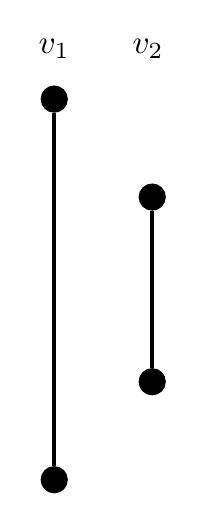
\begin{tikzpicture}[point/.style={circle, draw=black!100, fill=black!100, minimum size=2mm, align=center}]
            \node[point] (v_1_0) {};
            \node[above = 2mm of v_1_0, scale=1.2] (v_1_label) {$v_1$};
            \node[right = 5mm of v_1_label, scale=1.2] (v_2_label) {$v_2$};
            \node[point, below right = of v_1_0] (v_2_0) {};
            \node[point, below = 20mm of v_2_0] (v_2_1) {};
            \node[point, below left = of v_2_1] (v_1_1) {};
    
            \draw[-, ultra thick] (v_1_0) -- (v_1_1);
            \draw[-, ultra thick] (v_2_0) -- (v_2_1);
        \end{tikzpicture}
    \end{subfigure}
    \begin{subfigure}{0.45\textwidth}
        \centering
        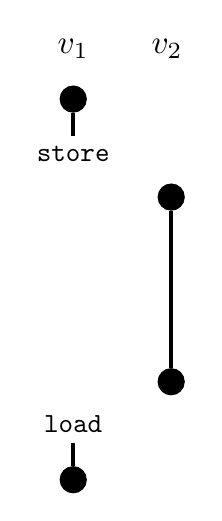
\begin{tikzpicture}[point/.style={circle, draw=black!100, fill=black!100, minimum size=2mm, align=center}]
            \node[point] (v_1_0) {};
            \node[above = 2mm of v_1_0, scale=1.2] (v_1_label) {$v_1$};
            \node[right = 5mm of v_1_label, scale=1.2] (v_2_label) {$v_2$};
            \node[point, below right = of v_1_0] (v_2_0) {};
            \node[below = 3mm of v_1_0] (store) {\texttt{store}};
            \node[point, below = 20mm of v_2_0] (v_2_1) {};
            \node[point, below left = of v_2_1] (v_1_1) {};
            \node[above = 3mm of v_1_1] (load) {\texttt{load}};
    
            \draw[-, ultra thick] (v_1_0) -- (store);
            \draw[-, ultra thick] (v_1_1) -- (load);
            \draw[-, ultra thick] (v_2_0) -- (v_2_1);
        \end{tikzpicture}
    \end{subfigure}
    \caption{Exemplo de \textit{splitting}. Nesse caso, $v_1$ é dividido ao redor de $v_2$, eliminando a interferência.}
    \label{fig:splitting-1}
\end{figure}

De modo a contemplar as relações de contenção entre os \textit{live ranges}, o \textit{live range splitting} requer a construção de um grafo direcionado $C$, denominado grafo de contenção. Os nós de $C$ representam as variáveis, enquanto uma aresta $e=(v_2,v_1)$ indica que $v_1$ estava vivo em uma definição ou uso de $v_2$. A Figura \ref{fig:splitting-2} exemplifica as possíveis relações entre os tempos de vida, baseado nos pontos onde são definidos e usados em relação uns aos outros.

\begin{figure}[ht]
    \centering
    \begin{subfigure}[t]{0.30\textwidth}
        \centering
        \adjustbox{valign=t}{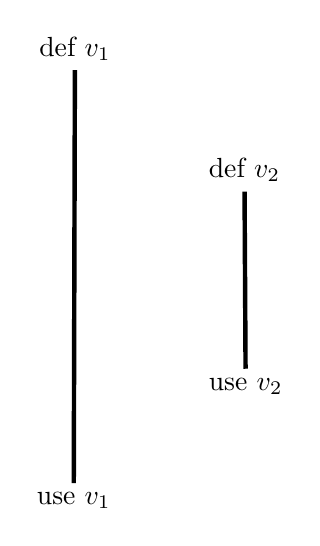
\begin{tikzpicture}
            \node (v_1_0) {def $v_1$};
            \node[below right = of v_1_0] (v_2_0) {def $v_2$};
            \node[below left = of v_2_0] (use) {};
            \node[below right = of use] (v_2_1) {use $v_2$};
            \node[below left = of v_2_1] (v_1_1) {use $v_1$};

            \draw[-, ultra thick] (v_1_0) -- (v_1_1);
            \draw[-, ultra thick] (v_2_0) -- (v_2_1);
        \end{tikzpicture}}
    \end{subfigure}
    \unskip\ \vrule\ 
    \begin{subfigure}[t]{0.30\textwidth}
        \centering
        \adjustbox{valign=t}{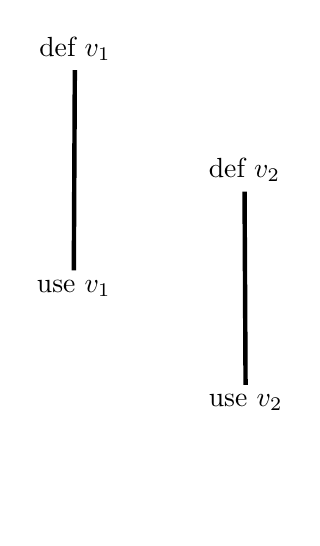
\begin{tikzpicture}
            \node (v_1_0) {def $v_1$};
            \node[below right = of v_1_0] (v_2_0) {def $v_2$};
            \node[below left = of v_2_0] (use) {use $v_1$};
            \node[below right = of use] (v_2_1) {use $v_2$};
            \node[below left = of v_2_1] (v_1_1) {};

            \draw[-, ultra thick] (v_1_0) -- (use);
            \draw[-, ultra thick] (v_2_0) -- (v_2_1);
        \end{tikzpicture}}
    \end{subfigure}
    \unskip\ \vrule\ 
    \begin{subfigure}[t]{0.30\textwidth}
        \centering
        \adjustbox{valign=t}{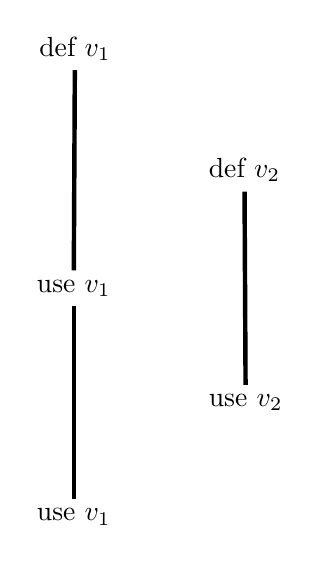
\begin{tikzpicture}
            \node (v_1_0) {def $v_1$};
            \node[below right = of v_1_0] (v_2_0) {def $v_2$};
            \node[below left = of v_2_0] (use) {use $v_1$};
            \node[below right = of use] (v_2_1) {use $v_2$};
            \node[below left = of v_2_1] (v_1_1) {use $v_1$};

            \draw[-, ultra thick] (v_1_0) -- (use);
            \draw[-, ultra thick] (v_1_1) -- (use);
            \draw[-, ultra thick] (v_2_0) -- (v_2_1);
        \end{tikzpicture}}
    \end{subfigure} \\
    \begin{subfigure}[b]{0.3\textwidth}
        \centering
        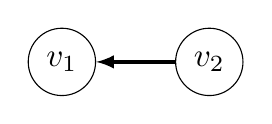
\begin{tikzpicture}[C/.style={draw,circle, scale=1.2}]
            \node[C] (v_1) {$v_1$};
            \node[C, right = of v_1] (v_2) {$v_2$};

            \draw[-latex, very thick] (v_2) -- (v_1);
        \end{tikzpicture}
        \caption{}
        \label{fig:splitting-2:a}
    \end{subfigure}
    \begin{subfigure}[b]{0.3\textwidth}
        \centering
        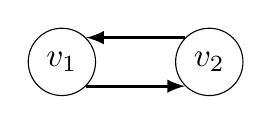
\begin{tikzpicture}[C/.style={draw,circle, scale=1.2}]
            \node[C] (v_1) {$v_1$};
            \node[C, right = of v_1] (v_2) {$v_2$};
            \draw[-latex, very thick] (v_2.north west) -- (v_1.north east);
            \draw[-latex, very thick] (v_1.south east) -- (v_2.south west);
        \end{tikzpicture}
        \caption{}
        \label{fig:splitting-2:b}
    \end{subfigure}
    \begin{subfigure}[b]{0.3\textwidth}
        \centering
        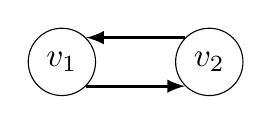
\begin{tikzpicture}[C/.style={draw,circle, scale=1.2}]
            \node[C] (v_1) {$v_1$};
            \node[C, right = of v_1] (v_2) {$v_2$};
            \draw[-latex, very thick] (v_2.north west) -- (v_1.north east);
            \draw[-latex, very thick] (v_1.south east) -- (v_2.south west);
        \end{tikzpicture}
        \caption{}
        \label{fig:splitting-2:c}
    \end{subfigure}
    \caption{Relações de contenção entre dois \textit{live ranges} e seus respectivos grafos. Adaptado de Cooper \textit{et al.} \cite{cooper:98}}
    \label{fig:splitting-2}
\end{figure}

A coluna \hyperref[fig:splitting-2:a]{(a)} mostra a mesma situação da Figura \ref{fig:splitting-1}, onde $v_2$ não está vivo em nenhum ponto de definição ou uso de $v_1$ e portanto está inteiramente contido em $v_1$, logo $(v_2,v_1) \in C$. Em \hyperref[fig:splitting-2:b]{(b)} ambas os \textit{live ranges} se sobrepõe, então ambos os caminhos $(v_1,v_2)$ e $(v_2,v_1)$ estão em $C$. O caso \hyperref[fig:splitting-2:c]{(c)} tem o mesmo resultado de \hyperref[fig:splitting-2:b]{(b)} devido à ocorrência de um uso de $v1$ em meio ao tempo de vida de $v_2$. A Tabela \ref{tab:splitting-1} resume as possibilidades de \textit{splitting} ou \textit{spilling} de acordo com a ocorrência de arestas no grafo de contenção $C$.

\begin{table}[hb]
    \centering
    % \begin{tabular*}{.65\textwidth}{@{\extracolsep{\fill}} c c}
    %     \hline
    %     \textbf{Arestas em $C$} & \textbf{Efeito na geração de \textit{spill code}} \\
    %     \hline
    %     $(v_i,v_j)$ & A divisão de $v_j$ ao redor de $v_i$ elimina\\
    %      & a interferência. O \textit{spill} de $v_i$, não.\\
    %     $(v_j,v_i)$ & A divisão de $v_i$ ao redor de $v_j$ elimina\\
    %      & a interferência. O \textit{spill} de $v_j$, não.\\
    %     $(v_i,v_j)$ e $(v_j,v_i)$ & Não se pode dividir nenhum dos dois.\\
    %      & Nenhum \textit{spill} remove a interferência. \\
    %      \hline
    % \end{tabular*}
    \begin{tabular}{cp{7cm}}
        \hline
        \textbf{Arestas em $C$} & \textbf{Efeito na geração de \textit{spill code}}\\\hline\hline
        $(v_i,v_j)$ & A divisão de $v_j$ ao redor de $v_i$ elimina a interferência. O \textit{spill} de $v_i$, não.\\\hline
        $(v_j,v_i)$ & A divisão de $v_i$ ao redor de $v_j$ elimina a interferência. O \textit{spill} de $v_j$, não.\\\hline
        $(v_i,v_j)$ e $(v_j,v_i)$ & Não se pode dividir nenhum dos dois. Nenhum \textit{spill} remove a interferência.\\\hline
    \end{tabular}
    \caption{Casos de \textit{splitting} de acordo com a ocorrência de arestas no grafo de conteção $C$. Adaptado de Cooper \textit{et al.} \cite{cooper:98}.}
    \label{tab:splitting-1}
\end{table}

Uma vez conhecidas as variáveis aptas a serem divididas com sucesso, o custo de fazê-lo deve ser computado pelo alocador para decidir entre \textit{spill} ou \textit{split}. O custo da divisão de cada \textit{live range} $v$ é obtido contando uma instrução \texttt{store} antes da definição e uma instrução \texttt{load} após o último uso, o que pode ser facilmente incorporado à fase de \textit{spill costs} de um alocador ao estilo Briggs. Caso $v$ seja escolhido para \textit{spill} durante a fase de seleção, uma cor deve ser encontrada para $v$ com base no custo de dividi-la em $v$ ou o contrário. Se uma cor for encontrada, $v$ a recebe e os tempos de vida correspondentes são marcados para divisão.

Foram realizados experimentos com 32 \textit{benchmarks} e obteve-se resultados positivos na maioria deles. Em alguns casos, a diminuição na contagem de instruções de acesso à memória chegou a 78\%. No entanto, dois casos de teste apresentaram uma maior inserção de \textit{spill code}, e o \textit{live range splitting} obteve piores resultados quando comparado ao \textit{spilling} por região de interferência para mais da metade dos casos. Apesar disso, Cooper \textit{et al.} ressaltaram a viabilidade de combinar ambas as técnicas em um alocador capaz de decidir qual delas utilizar.

\section{\textit{Outras Técnicas}}

\textbf{Coloração prioritária} --- Chow \textit{et al.} publicaram em 1984 um trabalho descrevendo um algoritmo de coloração de grafos similar ao de Chaitin \cite{chaitin:82}, mas com a aplicação de uma heurística de prioridade para a etapa de seleção. O alocador computa a diferença de custo entre se armazenar uma variável na memória ou e em um registrador físico e, no processo de coloração, é dada prioridade aos vértices cujo custo do \textit{live range} associado é o mais promissor. Experimentos foram realizados em 13 \textit{benchmarks} consistindo de programas Pascal e Fortran, e foi observada uma melhora média de 39\% no tempo de execução dos binários gerados.

\chapter{Inteligência Artificial}

A inteligência artificial (IA) é uma área da ciência da computação que se encarrega de pesquisar e desenvolver sistemas computacionais capazes de desempenhar tarefas que, tipicamente, requereriam a inteligência humana. Os sistemas de IA são projetados para imitar ou mesmo superar os humanos em determinados domínios, exibindo habilidades análogas de raciocínio, representação de conhecimento, planejamento, entendimento de linguagem natural, percepção, aprendizagem e a capacidade de se mover e manipular objetos \cite{russell:21}.

Para atingir esses objetivos, os pesquisadores e desenvolvedores de IA apropriaram-se de uma vasta gama de técnicas, incluindo busca e otimização matemática, lógica formal, redes neurais artificiais e métodos baseados em estatística, pesquisa operacional e economia. Graças a esses fundamentos, as abordagens de IA são particularmente úteis para problemas nos quais uma solução algorítmica exata não está disponível, incluindo problemas de otimização NP-completos \cite{russell:21} como a alocação de registradores.

Sendo assim, este capítulo tem por objetivo fundamentar os conceitos por trás das principais técnicas de inteligência artificial empregadas nas pesquisas envolvendo alocação de registradores, que serão abordadas no Capítulo \ref{sec:trabalhos-correlatos}. Em específico, serão explanadas as áreas de aprendizado de máquina, redes neurais artificiais e algoritmos evolutivos.

\section{Aprendizado de Máquina}

O aprendizado de máquina ou \textit{``machine learning''} (ML), em inglês, é uma área da inteligência artificial que se encarrega do desenvolvimento de agentes inteligentes que se tornam aptos a realizar tarefas aprimorando-se a partir de dados, ao invés de serem explicitamente programados. Esse processo de aprimoramento é denominado ``aprendizado'' ou ``treinamento'', e envolve a utilização de um conjunto de dados a respeito da tarefa a ser efetuada e que são utilizados para melhorar a precisão do agente \cite{alzubi:18}.

O aprendizado de máquina é utilizado em situações em que há uma grande disponibilidade de dados. Através da análise desses dados e apoiando-se em fundamentos da estatística e probabilidade, é possível obter uma aproximação suficientemente precisa dos resultados esperados \cite{alpaydin:20}. A Figura \ref{fig:ml-esquema} ilustra o processo de desenvolvimento de um modelo genérico de \textit{machine learning}, desde o preparo dos dados até a etapa de avaliação da performance do agente inteligente.

\begin{figure}[htb]
    \centering
    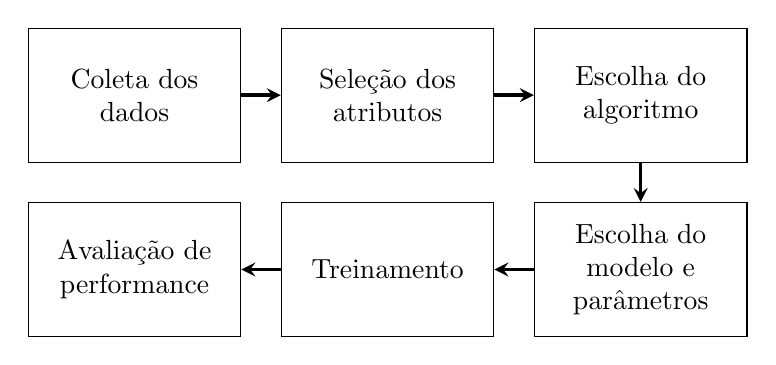
\begin{tikzpicture}[
        node distance= 0.5cm and 0.5cm,
        node/.style={draw, align=center, minimum width=2.7cm, minimum height=1.7cm},
        arrow/.style={very thick, ->, >=stealth}, scale=0.5
    ]
        \node[node] (n0) {Coleta dos\\dados};
        \node[node, right = of n0] (n1) {Seleção dos\\atributos};
        \node[node, right = of n1] (n2) {Escolha do\\algoritmo};
        \node[node, below = of n2] (n3) {Escolha do\\modelo e\\parâmetros};
        \node[node, left = of n3] (n4) {Treinamento};
        \node[node, left = of n4] (n5) {Avaliação de\\performance};

        \draw[arrow] (n0) -- (n1);
        \draw[arrow] (n1) -- (n2);
        \draw[arrow] (n2) -- (n3);
        \draw[arrow] (n3) -- (n4);
        \draw[arrow] (n4) -- (n5);
    \end{tikzpicture}
    \caption{Esquema ilustrando o desenvolvimento de um modelo genérico de \textit{machine learning}. Adaptado de Alzubi \textit{et al.} \cite{alzubi:18}.}
    \label{fig:ml-esquema}
\end{figure}

Sendo assim, as soluções do aprendizado de máquina consistem da identificação de padrões regulares na natureza do problema e na utilização desses padrões para realizar predições. Dentre as tarefas mais comuns dos modelos de \textit{machine learning} encontram-se \cite{alzubi:18}:

\begin{itemize}
    \item \textbf{Classificação} --- classificar os dados de entrada em um conjunto fixo de classes de saída conhecidos antecipadamente como sim ou não, verdadeiro ou falso, dentre outras;
    \item \textbf{Detecção de anomalias} --- buscar padrões nos dados de entrada de modo a identificar desvios ou anomalias. Exemplos reais incluem análise de tráfego de rede e identificação de transações fraudulentas;
    \item \textbf{Regressão} --- encontrar uma função matemática que descreva o resultado para uma dada entrada, com base nos dados disponíveis para treinamento. Exemplos são a estimativa de tendências de crescimento de preços ou crescimento populacional;
    \item \textbf{Agrupamento} --- encontrar estruturas nos dados e separá-los em grupos. Um exemplo real é a análise de texto para agrupá-los por classe de documentos semelhantes.
\end{itemize}

O processo de aprendizado em si varia conforme as informações disponíveis e as demandas da tarefa, e consiste num processo iterativo e contínuo. Ele pode ou não envolver o tratamento de grandes quantidades de dados por parte de um intérprete humano, ou mesmo por outro modelo de inteligência artificial, e depende das decisões de projeto tomadas pelos desenvolvedores de ``machine learning'' \cite{alpaydin:20, sharma:21}. Os principais paradigmas de aprendizado serão explorados nas subseções seguintes.

\subsection{Aprendizado Supervisionado}

No paradigma de aprendizado supervisionado, cada entrada do conjunto de dados de treinamento é rotulada de acordo com as variáveis relevantes ao processo de aprendizagem. Em termos formais, cada elemento do conjunto de treinamento é definido como composto pelo vetor das variáveis de entrada $\Vec{X}$ e um rótulo $r$, tal que o conjunto de treinamento seja caracterizado por um mapeamento $m : \Vec{X} \to \{r_1, r_2, \dots, r_n\}$. O processo de treinamento então visa ajustar o modelo para produzir um mapeamento $m' : \Vec{X} \to \{r_1, r_2, \dots, r_n\}$, onde $m'$ é suficientemente próximo da relação $m$ original presente no conjunto de treinamento \cite{mohammed:16, alpaydin:20}.

Neste contexto, os rótulos para o vetor de saída são fornecidos por um supervisor, que pode ser tanto um humano quanto uma máquina. Embora a rotulagem por humanos seja mais cara e demorada, os erros mais frequentes na rotulagem feita por máquinas sugerem a superioridade do julgamento humano. Dados rotulados manualmente são considerados recursos valiosos e confiáveis para o aprendizado supervisionado, embora em alguns casos, máquinas também possam ser usadas para rotulagem confiável \cite{mohammed:16}.

Na Figura \ref{fig:plot-supervisionado}, um conjunto de treinamento contendo 4 elementos, cada qual formado por um vetor de entrada $\Vec{X} = [x_1,x_2]^T$ e rotulado como $\{r_1, r_2\}$, forma um espaço bidimensional. Após um treinamento supervisionado um modelo inteligente encontra a classificação $C$, que compreende os elementos do conjunto que possuem o rótulo $r_1$. A Tabela \ref{tab:rotulos} demonstra possíveis rotulações para conjuntos de dados não-rotulados, a serem atribuídos por um agente supervisor.

\begin{figure}[hbt]
    \centering
    \begin{tikzpicture}[scale=1.2]
        % Eixos como réguas
        \draw[->] (0, 0) -- (5.5, 0) node[right] {$x_1$};
        \draw[->] (0, 0) -- (0, 5.5) node[above] {$x_2$};
        
        % Pontos no primeiro quadrante
        \foreach \x/\y/\label in {1/1/r_2, 3/2/r_1, 2/4/r_1, 4/3/r_1}
        {
        \fill (\x, \y) circle (2pt) node[above right] {$\label$};
        }
        
        \draw[dashed] (1.5, 1.5) rectangle (4.5, 4.5) node[above right] {$C$};
    \end{tikzpicture}
    \caption{Análise gráfica considerando um conjunto de treinamento com 4 elementos, formados pelos parâmetros de entrada $\Vec{X} = [x_1,x_2]^T$ e rótulos $\{r_1, r_2\}$.}
    \label{fig:plot-supervisionado}
\end{figure}

\begin{table}[htb]
    \centering
    \begin{tabular}{ccc}
        \hline
        \textbf{Exemplo de dado} & \textbf{Critério de rotulação} & \textbf{Possíveis rótulos} \\ \hline
        \textit{Tweet} & Sentimento do \textit{tweet} & $\{\text{positivo},\text{negativo}\}$ \\
        Imagem & Contém uma casa ou carro? & $\{\text{sim},\text{não}\}$ \\
        Áudio & A palavra ``futebol'' é dita & $\{\text{sim},\text{não}\}$ \\
        Vídeo & Armas são mostradas no vídeo? & $\{\text{violento},\text{não-violento}\}$ \\
        Raio X & Presença de tumor no raio X & $\{\text{presente},\text{ausente}\}$ \\
        \hline
    \end{tabular}
    \caption{Exemplos de dados não-rotulados e possíveis critérios de rotulação a um possível supervisor. Extraído de Mohammed \textit{et al.} \cite{mohammed:16}}
    \label{tab:rotulos}
\end{table}

\subsection{Aprendizado Não-Supervisionado}

No paradigma não-supervisionado, não há um supervisor para rotular os elementos do conjunto de entrada. Essa abordagem foca em reconhecer padrões não identificados previamente nos dados para derivar os critérios de classificação ou regressão a partir deles. Essa técnica é adequada para processar grandes volumes de dados onde a rotulação é demasiado trabalhosa ou impossível, realizando análises estatísticas para descobrir estruturas ocultas em dados não-rotulados \cite{mohammed:16}. 

Dentre os principais métodos de aprendizado não-supervisionado destacam-se o agrupamento (\textit{clustering}) e a redução de dimensionalidade. O agrupamento envolve a tarefa de identificar grupos ou \textit{clusters} de dados semelhantes com base em suas características, permitindo a segmentação de dados em categorias não conhecidas previamente. A redução de dimensionalidade busca representar dados complexos em um espaço de menor dimensão, preservando as características importantes, o que é útil para simplificar a análise de dados de alta dimensionalidade e visualização \cite{usama:19}. 

Algoritmos populares incluem o $k$-\textit{means} para agrupamento, que divide os dados em \textit{clusters}, ou agrupamentos, com base na proximidade dos pontos de dados uns com os outros espaço $n$-dimensional \cite{alpaydin:20, mohammed:16}, e a análise de componentes principais (PCA) para redução de dimensionalidade, que é uma técnica que reduz a dimensionalidade dos dados, mantendo as informações mais importantes e descartando as menos importantes \cite{gorban:10}. 

A Figura \ref{fig:k-means} mostra dados plotados em 2 dimensões divididos em 2 \textit{clusters}, cujos centroides \footnote{O centroide corresponde ao ponto médio de todos os elementos de um determinado agrupamento no espaço $k$-dimensional.} são indicados por um ``$\times$''. A Figura \ref{fig:pca} mostra uma visualização de um conjunto de dados de \textit{microarray} sobre câncer de mama usando mapas elásticos. O \textit{plot} (a) mostra nós projetados em um espaço tridimensional; o conjunto de dados é curvo e não pode ser adequadamente mapeado em um plano principal bidimensional. O \textit{plot} (b) mostra a distribuição nas coordenadas internas da superfície principal não linear bidimensional e (c) o mesmo que (b), mas para o espaço linear bidimensional após realização do PCA.

\begin{figure}[hbt]
    \centering
    \includegraphics[width=.6\textwidth]{pca}
    \caption{\textit{Plot} de um conjunto de dados de \textit{microarray} de câncer de mama usando mapas elásticos, empregando técnicas de análise de componentes principais. Extraído de Gorban e Zinovyev \cite{gorban:10}.}
    \label{fig:pca}
\end{figure}

\begin{figure}[hbt]
    \centering
    \includegraphics[width=.5\textwidth]{k-means}
    \caption{Exemplo de aplicação do $k$-\textit{means}. Os centroides dos \textit{clusters} são indicados com um ``$\times$'' no gráfico. Extraído de Alpaydin \cite{alpaydin:20}.}
    \label{fig:k-means}
\end{figure}

\subsection{Aprendizado Semi-supervisionado}

No aprendizado semi-supervisionado os dados fornecidos consistem em uma mistura de dados rotulados e não rotulados. Essa combinação de ambos os tipos é usada para criar um modelo apropriado para a classificação de dados sendo que, frequentemente, os dados rotulados são escassos, enquanto os não rotulados são abundantes. O objetivo da classificação semi-supervisionada é aprender um modelo que preveja as classes de dados de teste futuros melhor do que um modelo gerado apenas com os dados rotulados. Isso permite aproveitar ao máximo os dados não rotulados disponíveis para melhorar o desempenho da classificação \cite{mohammed:16}.

Alguns dos principais métodos de treinamento empregados no aprendizado semi-supervisionado incluem, dentre outros \cite{prakash:14, vanengelen:20}: 

\begin{itemize}
    \item \textbf{Modelos generativos} --- visam aprender a distribuição de probabilidade dos dados não rotulados com base nos dados rotulados conhecidos. Eles permitem não apenas fazer previsões ou classificações, mas também gerar novos dados que se assemelham aos dados de treinamento. Esses modelos são úteis para a geração de dados sintéticos e para melhorar o desempenho da classificação;
    \item \textit{\textbf{Self-training}} --- um agente classificador é treinado usando os dados rotulados, e em seguida é usado para rotular o restante dos dados não classificados do conjunto de treinamento;
    \item \textit{\textbf{Co-training}} --- se baseia na ideia de usar múltiplas visualizações ou conjuntos de características dos dados para treinar modelos independentes. Essa abordagem é particularmente útil quando os dados disponíveis podem ser divididos em diferentes visualizações que fornecem informações complementares.
\end{itemize}

\subsection{Aprendizado por Reforço}

No aprendizado por reforço, o agente inteligente toma decisões em um ambiente e recebe recompensas (ou penalidades) por suas ações ao tentar resolver um problema e, após uma série de tentativas e erros, o agente deve apresentar a melhor política de tomada de decisões, que é a sequência de ações que maximiza a recompensa total \cite{alpaydin:20}. A política é dada pelo mapeamento $\pi : A \times S \to [0,1]$, onde $A$ é o conjunto das ações e $S$ é o conjunto dos estados do sistema. A política $\pi(a,s)$ retorna a probabilidade da ação $a \in A$ ser tomada dado o estado $s \in S$ do ambiente \cite{kaelbiling:96}.

O treinamento se dá de maneira iterativa, quando o agente observa o estado de entrada no ambiente e, em seguida, utiliza uma função de tomada de decisão para escolher e realizar uma ação específica. Após a execução da ação, o agente recebe uma recompensa ou reforço do ambiente, que pode ser positiva (indicando uma ação benéfica) ou negativa (indicando uma ação prejudicial). A geração de políticas de tomada de decisão pode ser feita através de força-bruta ou empregando heurísticas fundamentadas em processos estocásticos para a escolha da próxima ação, se baseando nas ações prévias do sistema e o atual estado \cite{mohammed:16, kaelbiling:96}, sendo que esse processo é ilustrado pela Figura \ref{fig:rl}.

\begin{figure}[hbt]
    \centering
    % \includegraphics[scale=1.2]{rl}
    \begin{tikzpicture}
        \node (agente) {
            \adjustbox{scale=0.7}{\begin{tikzpicture}[text centered, draw=black, node distance=1.5cm, >=Stealth, thick]
            
            % Camada de entrada
            \foreach \i in {1,...,4}
                \node[circle, draw, minimum size=0.75cm] (I-\i) at (0,-\i) {};
            
            % Camada oculta
            \foreach \h [count=\hi] in {1,...,4} % Ajuste o número de nós na camada oculta
                \node[circle, draw, minimum size=0.75cm, right = 1cm of I-\h] (H-\h) {};
    
            % Conexões entre camadas
            \foreach \i in {1,...,4}
                \foreach \h in {1,...,4}
                    \draw[-] (I-\i) -- (H-\h);
            \end{tikzpicture}}
            };
        \node[above = 1mm of agente] {Agente};
        \coordinate[right = 35mm of agente] (a);
        \node[draw, right = 35mm of a, minimum width = 1cm, minimum height = 3cm] (ambiente) {Ambiente};
        \node[below = 30mm of a, draw, circle] (inter) {Intérprete};

        \draw[->, -latex, very thick] (agente) -- node[above=1mm] {Ação} (ambiente);
        \path[->, -latex, very thick] (ambiente.south) edge[bend left] (inter);
        \path[->, -latex, very thick] (inter) edge[bend left] node[right=3mm] {Estado} (agente.290);
        \path[->, -latex, very thick] (inter) edge[bend left] node[left=3mm] {\textit{Feedback}} (agente.250);
    \end{tikzpicture}
    \caption{Esquema do processo de treinamento via aprendizado por reforço.}
    \label{fig:rl}
\end{figure}

O aprendizado por reforço difere dos outros paradigmas de aprendizado de várias maneiras; a diferença mais importante é a não utilização de pares de entrada/saída esperada, como no aprendizado supervisionado. Em vez disso, depois de escolher uma ação, o agente é informado sobre a recompensa imediata e o estado subsequente, mas não é informado sobre qual ação teria sido do seu melhor interesse a longo prazo. É necessário para o agente adquirir experiência útil sobre os possíveis estados do sistema, ações, transições e recompensas ativamente para agir de forma otimizada. Outra diferença em relação ao aprendizado supervisionado é que o desempenho em tempo real é importante: a avaliação do sistema muitas vezes ocorre simultaneamente ao aprendizado \cite{kaelbiling:96}.

\section{Redes Neurais Artificiais e Aprendizado Profundo}

As redes neurais artificiais (ANNs) constituem uma classe de modelos de inteligência artificial que têm como inspiração para sua estrutura o funcionamento do cérebro humano. As redes neurais são compostas de uma série de unidades chamadas neurônios, que individualmente realizam operações matemáticas simples, e de sinapses que representam as conexões entre os neurônios. 

Cada neurônio artificial funciona realizando uma soma ponderada dos valores de entrada associados cada um ao peso da sinapse, e computando uma função matemática, chamada de função de ativação, que produz uma saída propagada para a camada seguinte. Sendo assim, uma rede neural possui ao menos uma camada de entrada e uma camada de saída, que apresenta o resultado \cite{krogh:08, mathew:21}. A Figura \ref{fig:neuronio} esquematiza um neurônio artificial que recebe como entrada os valores $x_1$, $x_2$, $\dots$, $x_n$, cada qual associado a um peso $w_1$, $w_2$, $\dots$, $w_n$. O somatório é adicionado a um valor $b$ conhecido como viés ou limiar, e é submetido a uma função de ativação não-linear $f$.

\begin{figure}[hbt]
    \centering
    \adjustbox{scale=1.2}{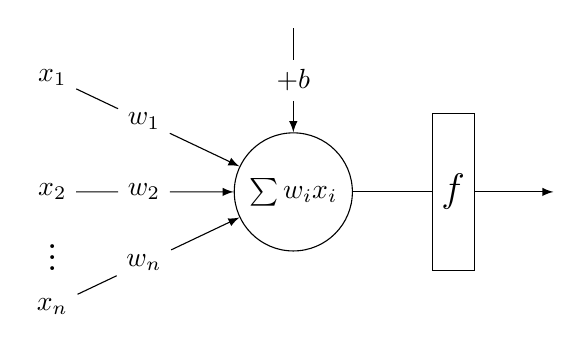
\begin{tikzpicture}[text centered]
        \node (x_1) {$x_1$};
        \node[below = of x_1] (x_2) {$x_2$};
        \node[below = of x_2] (x_3) {$x_n$};

        \coordinate (intermediate) at ($(x_2)!0.5!(x_3)$);
        \node[text centered] (c) at (intermediate) {\Large $\vdots$};
        
        \node[right = 2cm of x_2, circle, draw=black, minimum width=1.5cm] (neuronio) {$\sum w_ix_i$};
        \node[above = 0.4cm of neuronio] (b) {$+b$};
        \coordinate[above = 0.4cm of b] (l);
    
        \coordinate (c1) at ($(x_1)!0.38!(neuronio)$);
        \coordinate (c2) at ($(x_2)!0.38!(neuronio)$);
        \coordinate (c3) at ($(x_3)!0.38!(neuronio)$);
        
        \node (w1) at (c1) {$w_1$};
        \node (w2) at (c2) {$w_2$};
        \node (w3) at (c3) {$w_n$};
        
        \node[right = of neuronio, draw, minimum width = 0.5cm, minimum height = 2cm] (vies) {\Large $f$};
        
        \draw[-] (x_1) -- (w1);
        \draw[->,-latex] (w1) -- (neuronio);
        \draw[-] (x_2) -- (w2);
        \draw[->,-latex] (w2) -- (neuronio);
        \draw[-] (x_3) -- (w3);
        \draw[->,-latex] (w3) -- (neuronio);

        \draw[-] (l) -- (b);
        \draw[->,-latex] (b) -- (neuronio);

        \draw[-] (neuronio) -- (vies);
        \coordinate[right = 1cm of vies] (a);
        \draw[->,-latex] (vies) -- (a);
    \end{tikzpicture}}
    \caption{Esquema do funcionamento básico de um neurônio artificial.}
    \label{fig:neuronio}
\end{figure}

As redes neurais que resolvem problemas de classificação são chamadas de ``\textit{percéptrons}'', ao dividir o espaço dos valores de entrada com uma série de hiperplanos\footnote{Generalização do conceito de plano para dimensões maiores. Dado um espaço $k$-dimensional, um hiperplano é um subespaço $k-1$-dimensional. O correspondente a um hiperplano em um espaço bidimensional é uma reta; em um espaço tridimensional, é um plano propriamente dito.}, onde os valores de cada lado dos hiperplanos pertencem a classes distintas. Problemas nos quais é necessário o uso de somente um hiperplano são ditos linearmente separáveis, e podem ser resolvidos por redes neurais simples. Entretanto, grande parte dos problemas reais não são linearmente separáveis. Nesses casos, é necessário a utilização de mais hiperplanos através da introdução de camadas ocultas na rede neural que realizam, cada uma, classificações parciais que são repassadas à camada seguinte, até que se chegue na camada final \cite{krogh:08, alpaydin:20}.

\begin{figure}[hbt]
    \centering
    \begin{subfigure}{.49\textwidth}
        \centering
        \adjustbox{scale=1.4, valign=c}{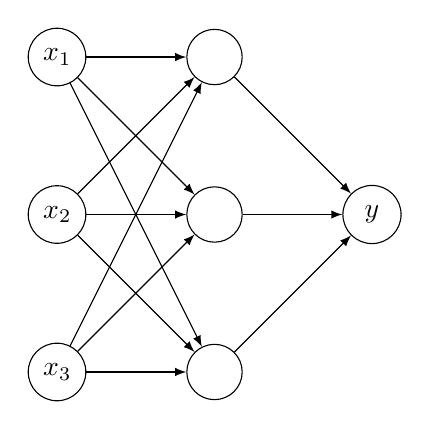
\begin{tikzpicture}[node distance=2cm,->,-latex]
            \node [draw, circle, text width=1em, text centered, minimum height=2em] (input1) {$x_1$};
            \node [draw, circle, text width=1em, text centered, minimum height=2em, below of=input1] (input2) {$x_2$};
            \node [draw, circle, text width=1em, text centered, minimum height=2em, below of=input2] (input3) {$x_3$};
            % Camada oculta
            \node [draw, circle, text width=1em, text centered, minimum height=2em, right of=input1] (hidden1) {};
            \node [draw, circle, text width=1em, text centered, minimum height=2em, right of=input2] (hidden2) {};
            \node [draw, circle, text width=1em, text centered, minimum height=2em, right of=input3] (hidden3) {};
            
            % Camada de saída
            \node [draw, circle, text width=1em, text centered, minimum height=2em, right of=hidden2] (output) {$y$};
            
            % Conexões
            \path (input1) edge (hidden1);
            \path (input1) edge (hidden2);
            \path (input1) edge (hidden3);
            \path (input2) edge (hidden1);
            \path (input2) edge (hidden2);
            \path (input2) edge (hidden3);
            \path (input3) edge (hidden1);
            \path (input3) edge (hidden2);
            \path (input3) edge (hidden3);
            \path (hidden1) edge (output);
            \path (hidden2) edge (output);
            \path (hidden3) edge (output);
        \end{tikzpicture}}
    \end{subfigure}
    \begin{subfigure}{.49\textwidth}
        \centering
        \adjustbox{scale=1.4, valign=c}{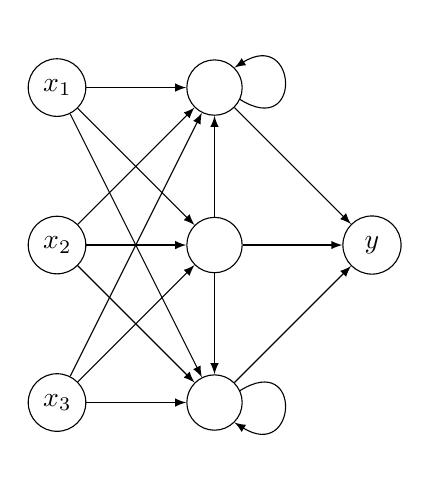
\begin{tikzpicture}[node distance=2cm,->,-latex]
            \node [draw, circle, text width=1em, text centered, minimum height=2em] (input1) {$x_1$};
            \node [draw, circle, text width=1em, text centered, minimum height=2em, below of=input1] (input2) {$x_2$};
            \node [draw, circle, text width=1em, text centered, minimum height=2em, below of=input2] (input3) {$x_3$};
            % Camada oculta
            \node [draw, circle, text width=1em, text centered, minimum height=2em, right of=input1] (hidden1) {};
            \node [draw, circle, text width=1em, text centered, minimum height=2em, right of=input2] (hidden2) {};
            \node [draw, circle, text width=1em, text centered, minimum height=2em, right of=input3] (hidden3) {};
            
            % Camada de saída
            \node [draw, circle, text width=1em, text centered, minimum height=2em, right of=hidden2] (output) {$y$};

            \coordinate[above right = 0.5cm and 0.8cm of hidden1.north east] (h1_b1);
            \coordinate[below right = 0.5cm and 0.8cm of hidden1.335] (h1_b2);
            \coordinate[above right = 0.5cm and 0.8cm of hidden3.25] (h2_b1);
            \coordinate[below right = 0.5cm and 0.8cm of hidden3.south east] (h2_b2);
            
            % Conexões
            \path (input1) edge (hidden1);
            \path (input1) edge (hidden2);
            \path (input1) edge (hidden3);
            \path (input2) edge (hidden1);
            \path (input2) edge (hidden2);
            \path (input2) edge (hidden3);
            \path (input3) edge (hidden1);
            \path (input3) edge (hidden2);
            \path (input3) edge (hidden3);
            \path (hidden1) edge (output);
            \path (hidden2) edge (output);
            \path (hidden3) edge (output);
            \path (hidden2) edge (hidden3);
            \path (hidden2) edge (hidden1);
            \draw[->, -latex] (hidden1.335) .. controls (h1_b2) and (h1_b1) .. (hidden1.north east);
            \draw[->, -latex] (hidden3.25) .. controls (h2_b1) and (h2_b2) .. (hidden3.south east);
        \end{tikzpicture}}
    \end{subfigure}    
    \caption{Uma rede neural \textit{feed-forward} e uma rede neural recorrente, na esquerda e direita respectivamente.}
    \label{fig:ann}
\end{figure}

Quando uma rede neural possui uma ou mais camadas intermediárias entre a entrada e a saída, ela é denominada ``rede neural profunda'', e seu processo de treinamento é chamado de aprendizado profundo, ou \textit{``deep learning''}. Como mostrado na Figura \ref{fig:ann}, as redes neurais profundas podem ter uma organização \textit{``feed-forward''}, forma mais amplamente utilizada e que apresenta um fluxo unidirecional de uma camada para outra, ou recorrente, que pode conter ciclos e possuir um fluxo bidirecional entre as camadas \cite{mathew:21}.

As funções de transferência geralmente possuem uma forma sigmoide, mas também podem adotar a forma de outras funções não-lineares, funções lineares em partes ou funções degrau. Algumas importantes funções usadas como limiar incluem \cite{sharma:20}:

\begin{itemize}
    \item \textbf{\textit{Função degrau}} --- saída binária, se a entrada for maior que um limite especificado $\theta$:
    \[f(x) = \begin{cases}
        1, & x \geq \theta\\
        0, & \text{caso contrário}.
    \end{cases}\]
    \item \textbf{\textit{Função logística}} --- função sigmoide (curva em forma de ``S''), utilizada para gerar um valor no intervalo $[0,1]$:
    \[
        f(x) = \frac{1}{1+e^{-x}}
    \]
    \item \textbf{\textit{Tangente hiperbólica}} --- função sigmoide com domínio limitado no intervalo $[-1,1]$, sendo simétrica em torno de $0$:
    \[
        f(x) = \tanh{x} = \frac{e^x - e^{-x}}{e^x + e^{-x}}
    \]
    \item \textbf{\textit{Rectified Linear Unit} (ReLU)} --- retorna a entrada se for positiva e zero caso contrário. É uma função de ativação popular em redes neurais profundas devido à eficiência no processo de treinamento:
    \[
        f(x) = \text{max }\{0, x\}
    \]
\end{itemize}

O treinamento dos modelos de rede neural pode ser feito através de um série de algoritmos, dentre os quais se destaca o método do \textit{back-propagation}, ou retropropagação, que faz uso de uma técnica de otimização numérica chamada descida gradiente para o treinamento de redes profundas \textit{feed-forward}. A rede é inicializada com todos os seus pesos recebendo valores aleatórios e a primeira iteração é realizada, onde uma entrada é analisada e é produzida uma saída aleatória. 

Em seguida, é calculado um erro, igual ao quadrado da diferença entre o último resultado e o resultado esperado, e os parâmetros da rede (pesos e limiares) são ajustados de modo a reduzir o erro calculado. Esse processo é repetido inúmeras vezes, até que se obtenha o conjunto de pesos que minimizam o erro e produzem um resultado muito próximo do esperado \cite{krogh:08}.

Redes neurais profundas, incluindo as \textit{feed-forward} e as recorrentes, desempenham um papel fundamental em uma ampla variedade de aplicações. Na visão computacional, elas são usadas para tarefas como detecção de objetos, reconhecimento facial e classificação de imagens. No processamento de linguagem natural, auxiliam na análise de sentimento, tradução automática, geração de texto e reconhecimento de fala. 

Já as redes neurais recorrentes destacam-se no processamento de sequências, como tradução automática e geração de texto coerente, bem como na modelagem de linguagem. A versatilidade do \textit{deep learning} e a capacidade de aprender padrões complexos apresentada pelas redes neurais profundas as tornam essenciais em muitos campos, e representam um grande horizonte a ser investigado nas pesquisas \cite{sharma:21}.

\section{Algoritmos Evolutivos}

Os algoritmos evolutivos constituem uma família de algoritmos para otimização meta-heurística que se inspiram no conceito de evolução biológica para encontrar soluções. Eles são utilizados na área da inteligência artificial para aperfeiçoar heurísticas de problemas de otimização não-linear complexos, com um funcionamento semelhante ao dos algoritmos de busca. Contudo, os algoritmos evolutivos trazem como diferencial a capacidade de buscar soluções em um espaço de amostragem aleatória, se caracterizando como um método de \textit{Monte Carlo}\footnote[1]{Os métodos de Monte Carlo são técnicas estocásticas que buscam estimar ou simular resultados determinísticos por meio de sucessivas amostragens aleatórias \cite{russell:21}.} \cite{ashlock:06}. % explicar o que é método de monte carlo

Servindo como base para a computação evolutiva, a evolução biológica é um fenômeno constatado por vários cientistas independentemente ao longo de séculos, mas formalizada mais notavelmente por Charles Darwin \cite{darwin:59}. Funcionando como um método de otimização, o processo evolutivo produziu toda a biodiversidade existente no planeta com suas sofisticadas, mas não perfeitas, soluções para a sobrevivência e reprodução dos seres vivos \cite{back:00}. Contudo, do ponto de vista biológico, a evolução pode ser definida simplesmente como a mudança das frequências de alelos em uma população ao longo do tempo \cite{ashlock:06}.

\begin{figure}[htb]
    \centering
    \includegraphics{convergencia}
    \caption{Paisagem de \textit{fitness} projetada em duas dimensões. A região mais clara indica um ótimo local, e os pontos demarcam os indivíduos que compõe a população. Ao longo de seis gerações, é possível visualizar a convergência em direção ao ponto de maior \textit{fitness}. Extraído de um trabalho de Corpus \textit{et al.} que utilizou estratégias evolutivas (ES) \cite{corpus:23}.}
    \label{fig:convergencia}
\end{figure}

A mudança na configuração genética de uma população ocorre através de dois principais mecanismos: variação e seleção. A variação é o processo pelo qual novos alelos são inseridos na população. Isso é possível graças à reprodução sexuada e de mutações pontuais, que modificam os genomas dos indivíduos de modo a introduzir variabilidade genética. Já o processo de seleção atua reduzindo a variabilidade genética, literalmente selecionando quais alelos se perpetuam na população com base na aptidão reprodutiva dos indivíduos que os possuem \cite{ashlock:06}.

Os algoritmos evolutivos, de maneira análoga, operam em populações de estruturas de dados. A variação insere alterações aleatórias em uma população de estruturas de dados recombinando partes de diferentes estruturas e ocasionalmente criando pequenas alterações pontuais. Esses dois processos são chamados respectivamente de cruzamento e mutação, e juntos são referidos como operadores de variação. A seleção é realizada com qualquer algoritmo que favoreça estruturas de dados com base em um critério de aptidão, ou \textit{fitness} \cite{ashlock:06, eiben:15}.

\begin{algoritmo}[htb]
    \begin{algorithmic}
        \caption{Algoritmo evolutivo genérico. Adaptado de Ashlock \cite{ashlock:06}.}
        \Procedure{AlgoritmoEvolutivo}{}
            \State $P \gets \text{\textbf{inicialize} uma população aleatória de estruturas de dados}$
            \Repeat
                \ForAll{indivíduo $i \in P$}
                    \State $\textit{fitness}[i] \gets$ \Call{AvaliarFitness}{i}
                \EndFor
                \State $P' \gets$ \Call{Seleção}{$P$, $\mathit{fitness}$}
                \State $P \gets$ \Call{Variação}{$P'$}
            \Until{o limite de gerações ser atingido}
        \EndProcedure
        \label{alg:evolutivo}
    \end{algorithmic}
\end{algoritmo}

O Algoritmo \ref{alg:evolutivo} exemplifica o funcionamento básico de um algoritmo evolutivo genérico. Um população de indivíduos é inicializada com uma amostragem aleatória de estrutura de dados, chamados de genomas ou cromossomos. Então, por um número determinado de gerações, são avaliados os valores de \textit{fitness} da população; o operador de seleção elimina os indivíduos com os piores \textit{fitness} e a variação é aplicada sobre os indivíduos resultantes de modo a produzir novos indivíduos. Cada categoria de algoritmo evolutivo é caracterizada por uma combinação de representação e operadores, que serão abordados posteriormente nesta seção \cite{ashlock:06, eiben:15}.

Com o passar das gerações, dado que boas técnicas de exploração e seleção de indivíduos aptos foram empregadas, haverá uma convergência da população em direção aos ótimos locais da paisagem adaptativa\footnote[1]{Conceito emprestado da biologia evolutiva, consiste na representação multidimensional da aptidão reprodutiva, ou \textit{fitness}, em função das variáveis sob processo evolutivo \cite{eiben:15}.} do problema, como mostrado pela Figura \ref{fig:convergencia}. Existem várias implementações diferentes de operadores de cruzamento, mutação e seleção, além das múltiplas possibilidades de escolha da estrutura de dados que representa os indivíduos \cite{back:00, eiben:15}.

\subsection{Cruzamento}

O operador de cruzamento, ou \textit{crossover}, é o principal responsável por introduzir variabilidade genética na população, ao permitir que os indivíduos troquem material genético para produzir novos genomas. Seja $G$ um cromossomo contido na população de estruturas, o operador de cruzamento $\chi$ é definido como o mapeamento de dois elementos no domínio, denominados ancestrais, para um (Definição \ref{eq:cruzamento-1}) ou dois (Definição \ref{eq:cruzamento-2}) pontos na imagem denominados descendentes \cite{ashlock:06}.

\begin{equation}
    \chi : G \times G \to G
    \label{eq:cruzamento-1}
\end{equation}

\begin{equation}
    \chi : G \times G \to G \times G
    \label{eq:cruzamento-2}
\end{equation}

A forma geral de um cruzamento consiste em particionar os genomas de ambos os ancestrais ao redor de um ou mais pontos escolhidos aleatoriamente, denominados lócus (loci no plural), e recombinar as partições para gerar novos genomas. Contudo, implementações mais exóticas podem ser concebidas a depender da estrutura de dados escolhida como representação dos genomas, contanto que o algoritmo garanta que os descendentes sejam compostos por partes herdadas de ambos ancestrais \cite{ashlock:06}. A Figura \ref{fig:crossover} exemplifica um cruzamento de dois pontos.

\begin{figure}[htb]
    \centering
    \includegraphics[scale=1.4]{crossover}
    \caption{Exemplo de cruzamento com dois pontos ou loci, entre genomas representados como \textit{strings} binárias. Extraído de Eiben e Smith \cite{eiben:15}.}
    \label{fig:crossover}
\end{figure}

O uso de vários pontos reduz o viés de herança do meio de representação, ao permitir que porções menores do genoma variem individualmente. Em último caso, pode ser efetuado cruzamento uniforme, onde a chance de um indivíduo herdar material genético de um ou outro ancestral é avaliada individualmente para cada lócus do genoma, com igual probabilidade de herança para ambos os ancestrais \cite{back:00}.

\subsection{Mutação}

O operador de mutação é o responsável por causar pequenas alterações no genoma de um único indivíduo. Enquanto o cruzamento é responsável por permitir a busca pelo espaço de soluções, as mutações são responsáveis por introduzir novos alelos que não evoluiriam com somente cruzamentos. Essa habilidade é útil porque permite que o algoritmo escape de ótimos locais e encontre melhores soluções. O operador de mutação $\sigma$ pode ser definido, então, como na Definição \ref{eq:mutacao} \cite{ashlock:06, eiben:15}.

\begin{equation}
    \sigma : G \to G
    \label{eq:mutacao}
\end{equation}

A forma básica de mutação é implementada como uma alteração na informação codificada em algum ponto do genoma. A partir desse conceito, operadores mais sofisticados podem ser derivados, como mutação em múltiplos pontos ou mutação probabilística, onde o genoma é percorrido e cada posição possui uma probabilidade $\alpha$ de sofrer uma alteração \cite{ashlock:06}. A Figura \ref{fig:mutacao} exemplifica um genoma que sofre mutação em três loci.

\begin{figure}[htb]
    \centering
    \vspace{0.7cm}
    \includegraphics[scale=1.4]{mutacao}
    \vspace{0.7cm}
    \caption{Exemplo de mutação onde uma \textit{string} binária tem três bits invertidos aleatoriamente. Extraído de Eiben e Smith \cite{eiben:15}.}
    \label{fig:mutacao}
\end{figure}

\subsection{Seleção}

A seleção, ao contrário dos operadores de variação, não cria novas soluções, mas somente destaca os melhores indivíduos em uma população eliminando os menos aptos. Essa eliminação leva em conta uma avaliação da aptidão de cada solução, denominada \textit{fitness}. A avaliação do \textit{fitness} é a etapa que geralmente detém o maior custo computacional dos algoritmos evolutivos. De modo geral, é esperado que os indivíduos mais aptos tenham maior chance de serem selecionados, mas isso não necessariamente irá ocorrer, a depender do método de seleção utilizado \cite{back:00}.

Os algoritmos de seleção podem ser determinísticos, onde um número fixo dos melhores indivíduos é selecionado, ou probabilísticos, em que cada indivíduo possui uma probabilidade de seleção proporcional a seu \textit{fitness}. Os métodos probabilísticos, ou estocásticos, são preferíveis em muitos casos, pois a estocasticidade da seleção promove a variabilidade genética da população, enquanto que os métodos determinísticos tendem a convergir prematuramente devido aos vieses da população original \cite{back:00}. Dentre os algoritmos de seleção probabilísticos, destacam-se:
\begin{itemize}
    \item \textbf{Roleta} --- Na seleção por roleta, a probabilidade de cada indivíduo $i$ ser selecionado para reprodução é igual a $\frac{\mathit{fitness}(i)}{\sum \mathit{fitness}}$, ou seja, igual à fração que corresponde o seu valor de \textit{fitness} em relação ao somatório total da população. A Tabela \ref{tab:selecoes} mostra as probabilidades de escolha para uma população de seis indivíduos usando o método da roleta;
    \item \textbf{Ranque} --- Semelhante à seleção por roleta, exceto por determinar a probabilidade de seleção utilizando um valor de ranqueamento ao invés do \textit{fitness}. Os indivíduos são ordenados em ordem crescente de melhor \textit{fitness}, e a posição de cada indivíduo em razão do somatório de todas as posições $\frac{\mathit{ranque}(i)}{\sum \mathit{ranque}}$ é utilizada como probabilidade. É útil em casos onde a variância dos valores de \textit{fitness} na população é muito grande ou muito pequena. As probabilidades para este método também são mostradas na Tabela \ref{tab:selecoes};
    \item \textbf{Torneio} --- Nesse método, um subconjunto de tamanho predeterminado contendo $k$ indivíduos é escolhido aleatoriamente. Esses indivíduos competem entre si, e o vencedor, com o melhor \textit{fitness}, é selecionado para reprodução. O tamanho $k$ do torneio influencia a pressão seletiva: quanto maior, menor é a chance de indivíduos menos aptos serem selecionados.
\end{itemize}

\begin{table}[htb]
    \centering
    \begin{tabular}{cccc}
         \hline
         \textbf{\textit{Fitness}} & \textbf{Ranque} & $P_\text{roleta}$ & $P_\text{ranque}$ \\
         \hline
         $2,1$ & $1$ & $0,099$ & $0,048$ \\
         $3,6$ & $5$ & $0,169$ & $0,238$ \\
         $7,1$ & $6$ & $0,333$ & $0,286$ \\
         $2,4$ & $2$ & $0,113$ & $0,095$ \\
         $3,5$ & $4$ & $0,164$ & $0,190$ \\
         $2,6$ & $3$ & $0,122$ & $0,143$ \\
         \hline
    \end{tabular}
    \caption{Comparação das probabilidades de escolha em uma população de seis indivíduos, considerando os métodos de seleção proporcional. Adaptado de Ashlock \cite{ashlock:06}.}
    \label{tab:selecoes}
\end{table}

A etapa seleção pode ser efetuada antes ou depois dos operadores de variação. Especificamente, nos paradigmas de algoritmo genético (GA) e programação genética (GP), o operador de seleção é usualmente aplicado antes da variação, de modo a selecionar boas soluções e só então efetuar recombinação e mutação. Outras formas de algoritmo evolutivo, como na programação evolutiva (EP) e estratégias evolutivas (ES), preferem aplicar os operadores de variação primeiro \cite{back:00}.

Nas implementações que postergam a seleção, a etapa de variação produz um conjunto de descendentes distinto da população ancestral, sobre o qual o operador de seleção é aplicado. Nesses casos, indivíduos de um ou ambos os conjuntos devem ser selecionados para compor a próxima geração do processo evolutivo, podendo ser empregadas as estratégias $(\mu + \lambda)$ ou $(\mu, \lambda)$, onde $\mu$ e $\lambda$ são os tamanhos da população ancestral e descendente, respectivamente.

No método $(\mu + \lambda)$, são selecionadas as $\mu$ melhores soluções de um conjunto que inclui tanto os $\mu$ ancestrais quanto os $\lambda$ descendentes. Como ambas as populações são avaliadas, se realizada de forma determinística, esse esquema de seleção garante a preservação da melhor solução encontrada em qualquer iteração. Essa propriedade é denominada elitismo, e é utilizada para manter bons indivíduos sempre na população \cite{back:00}.

Em contrapartida, no método $(\mu, \lambda)$ são selecionadas as $\mu$ melhores soluções somente do conjunto de descendentes $\lambda$. Isso implica que $\lambda > \mu$ --- se ambos os parâmetros populacionais forem iguais, não há seleção; o algoritmo torna-se um passeio aleatório pelo espaço de soluções --- e os melhores indivíduos não tem garantia de se manterem na população. Sendo assim, essa estratégia promove uma exploração mais exaustiva quando comparada com a estratégia $(\mu + \lambda)$.

Os operadores de seleção também são caracterizados por um parâmetro denominado pressão seletiva. Ele é determinado pelo tempo de dominação da população, que representa o tempo necessário para que a solução com melhor \textit{fitness} ocupe toda a população. Sendo assim, se a pressão seletiva é alta, a população perde diversidade rapidamente, enquanto que se é baixa, a convergência é lenta. Thierens e Goldberg \cite{thierens:93} demonstraram uma relação entre a pressão seletiva e a probabilidade de recombinação, e que uma alta pressão seletiva deve ser acompanhada por uma alta probabilidade de recombinação para que o algoritmo evolutivo tenha sucesso \cite{back:00}.

\subsection{Algoritmo Genético}

O algoritmo genético (GA) é o tipo mais popular de algoritmo evolutivo, e emula de forma mais análoga os genomas reais e sua variação através do processo evolutivo. Idealizado nas décadas de 50 e 60 por Holland, Bremermann e Fraser \cite{holland:62, bremermann:62, fraser:57, holland:75}, ele é amplamente utilizado em áreas como aprendizado de máquina graças à sua habilidade de encontrar heurísticas para problemas de otimização. 

Nessa modalidade de algoritmo evolutivo, os indivíduos são comumente representados na forma de \textit{strings} binárias de tamanho fixo (Figuras \ref{fig:crossover} e \ref{fig:mutacao}), apesar de representações alfanuméricas também serem possíveis \cite{vikhar:16}. Essas representações, denominadas cromossomos ou genomas, são compostas por genes, tal que um gene consiste na codificação de um parâmetro do problema. Esses genes também chamados de variáveis de decisão e determinam uma ou mais características fenotípicas do indivíduo, ou pelo menos têm influência sobre elas \cite{eiben:15}. A Tabela \ref{tab:variaveis-decisao} exemplifica um cromossomo binário típico dos GAs.

\begin{table}[htb]
    \centering
    \begin{tabular}{|c||c|c|c|c|c|c|c|c|c|c|c|c|c|c|c|c|}
        \hline
        variáveis & \multicolumn{6}{c|}{$D_1 = 22$} & \multicolumn{5}{c|}{$D_2 = 29$} & \multicolumn{5}{c|}{$D_3 = 28$} \\
        \hline
        bits & 0 & 1 & 0 & 1 & 1 & 0 & 1 & 1 & 1 & 0 & 1 & 1 & 1 & 1 & 0 & 0 \\
        \hline
    \end{tabular}
    \caption{Cromossomo cujo conteúdo é mapeado para três variáveis de decisão $D_1$, $D_2$, $D_3$.}
    \label{tab:variaveis-decisao}
\end{table}

A operação de mutação atua ao aleatoriamente inverter alguns bits da \textit{string} de representação. O cruzamento é feito simplesmente recombinando partes do cromossomo após o particionamento em um número predeterminado de pontos. Tradicionalmente, os algoritmos genéticos aplicam seleção reprodutiva, isto é, os melhores indivíduos são selecionados antes da aplicação dos operadores de variação e, comumente, métodos estocásticos de seleção são utilizados \cite{back:00}.

\subsection{Programação Genética}

A programação genética (GP) é um paradigma de algoritmo evolutivo introduzido por Cramer e Koza em meados dos anos 1980 \cite{cramer:85, koza:89}, onde as estruturas de dados em processo adaptativo são programas de computador. Para isso, os cromossomos que correspondem aos indivíduos assumem a forma de árvores sintáticas, estruturas usadas por compiladores e interpretadores como representação interna de programas em compilação.
A avaliação do \textit{fitness} então consiste em transformar essas representações em código executável e coletar métricas de execução de cada um dos programas na população \cite{back:00}.

Mais especificamente, os nós das árvores sintáticas podem ser classificados como funções primitivas ou símbolos terminais. As funções primitivas correspondem a elementos do código como expressões aritméticas e de comparação, estruturas de controle e chamadas de função. Os terminais incluem elementos de valor constante ou variáveis avaliadas em tempo de execução, que servem como parâmetros do programa. Dessa maneira, as soluções estão contidas em um espaço formado por todas as possíveis composições recursivamente criadas a partir das funções primitivas e terminais disponíveis \cite{koza:94}.

\begin{figure}[htb]
    \centering
    \adjustbox{scale=1.2}{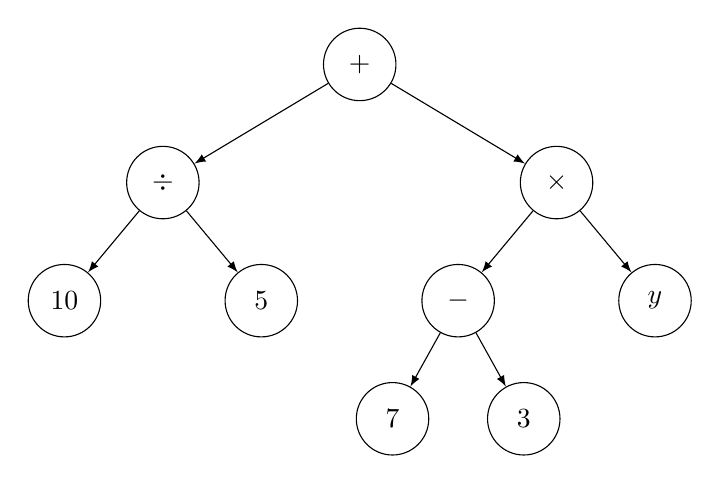
\begin{tikzpicture}[level/.style={sibling distance=50mm/#1},
                        every node/.style={draw, circle, minimum size=9.2mm},
                        edge from parent/.style={draw,-latex},
                        level distance=1.5cm]
        \node {$+$}
            child { node {$\div$}
                child { node {$10$} }
                child { node {$5$} }
            }
            child { node {$\times$} 
                child { node {$-$}
                    child { node {$7$} }
                    child { node {$3$} }
                }
                child { node {$y$} }
            };
    \end{tikzpicture}}\\ \vspace{0.2cm} \adjustbox{scale=1.2}{$+(\div(10,5),\times(-(7,3),y))$}
    \caption{Exemplo de árvore sintática com sua expressão correspondente, na comumente usada notação prefixa.}
    \label{fig:prog-genetica}
\end{figure}

Os símbolos disponíveis para a construção de árvores sintáticas também podem carregar significado semântico. Em uma instância de programação genética de tipagem forte, por exemplo, tanto os valores de retorno de um nó quanto os argumentos das funções primitivas possuem tipo, e a estrutura da árvore sintática deve respeitar essas restrições. Sendo assim, em uma instância fortemente tipada de programação genética onde a primitiva lógica $\lor$ possui dois operandos de tipo booleano, a expressão $1 \lor 0,45$ não configuraria um indivíduo válido no espaço de soluções, pois $0,45 \notin \{0,1\}$ \cite{eiben:15}.

A Figura \ref{fig:prog-genetica} mostra uma árvore sintática e a tradução para a expressão correspondente em notação prefixa. Os nós folha são formados por símbolos terminais, de valor constante ou variável, enquanto os nós intermediários são funções primitivas relacionadas aos operadores aritméticos. O paradigma da programação também genética traz consigo operadores próprios de cruzamento e mutação, apropriados para manipular a estrutura de árvore dos genomas. O operador de cruzamento atua recombinando ramos das árvores ancestrais para criar dois descendentes distintos, como mostrado na Figura \ref{fig:crossover-prog-genetica}. 

\begin{figure}[htb]
    \centering
    \begin{subfigure}{0.4\textwidth}
        \centering
        \adjustbox{valign=c}{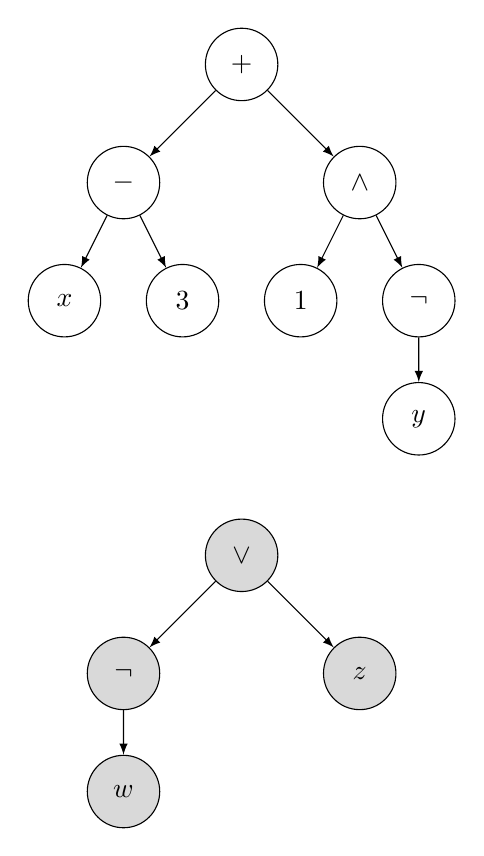
\begin{tikzpicture}[level/.style={sibling distance=30mm/#1},
                        every node/.style={draw, circle, minimum size=9.2mm},
                        edge from parent/.style={draw,-latex},
                        level distance=1.5cm]
            \node (+) {$+$}
                child { node {$-$}
                    child { node {$x$} }
                    child { node {$3$} }
                }
                child { node {$\land$} 
                    child { node {$1$} }
                    child { node {$\lnot$}
                        child { node {$y$} }
                    }
                };
            
            % Árvore 2
            \node[below=5.3cm of {+}, fill=gray!30] {$\lor$}
                child { node[fill=gray!30] {$\lnot$} 
                    child { node[fill=gray!30] {$w$} }
                }
                child { node[fill=gray!30] {$z$} };
        \end{tikzpicture}}
    \end{subfigure}
    \begin{subfigure}{0.18\textwidth}
        \centering
        \adjustbox{valign=c}{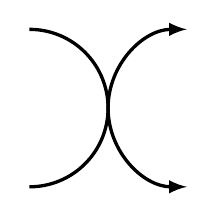
\begin{tikzpicture}
            \draw[-latex, very thick] (-1,-1) to[out=0, in=270] (0,0) to[out=90, in=180] (1,1); % Flecha de baixo para cima
            \draw[-latex,very thick] (-1,1) to[out=0, in=90] (0,0) to[out=270, in=180] (1,-1); % Flecha de cima para baixo
        \end{tikzpicture}}
    \end{subfigure}
    \begin{subfigure}{0.4\textwidth}
        \centering
        \adjustbox{valign=c}{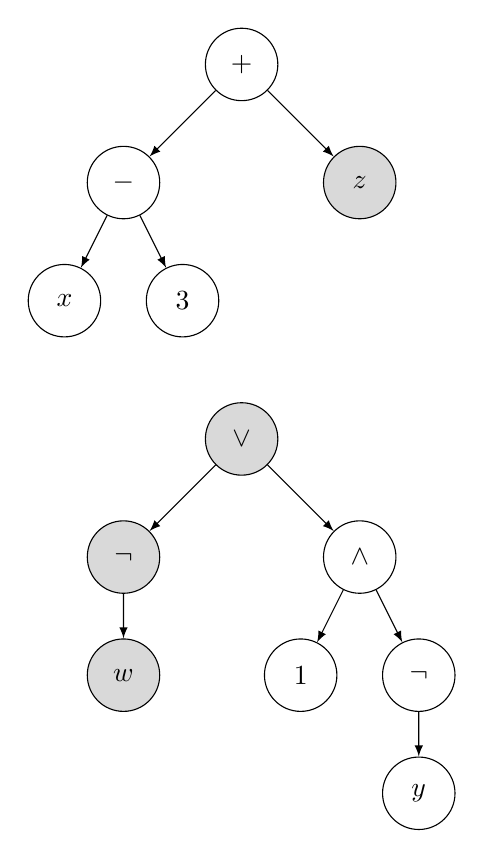
\begin{tikzpicture}[level/.style={sibling distance=30mm/#1},
                        every node/.style={draw, circle, minimum size=9.2mm},
                        edge from parent/.style={draw,-latex},
                        level distance=1.5cm]
            \node (+) {$+$}
                child { node {$-$}
                    child { node {$x$} }
                    child { node {$3$} }
                }
                child { node[fill=gray!30] {$z$} };
                
            \node [below=3.822cm of {+}, fill=gray!30] {$\lor$}
                child { node[fill=gray!30] {$\lnot$} 
                    child { node[fill=gray!30] {$w$} }
                }
                child { node {$\land$} 
                    child { node {$1$} }
                    child { node {$\lnot$}
                        child { node {$y$} }
                    }
                };
        \end{tikzpicture}}
    \end{subfigure}
    \caption{Demonstração do operador de cruzamento na programação genética. As subárvores $\land(1,\lnot(y))$ e $z$ são recombinadas para formar os indivíduos $+(-(x,3),z)$ e $\lor(\lnot(w),\land(1,\lnot(y)))$}
    \label{fig:crossover-prog-genetica}
\end{figure}

Já o operador de mutação realiza alterações aleatoriamente nos nós da árvore, podendo simplesmente alterar as primitivas e valores dos terminais, bem como inserir subárvores totalmente aleatórias em algum ponto do genoma do indivíduo mutante. A Figura \ref{fig:mutacao-prog-genetica} demonstra a substituição de um nó por uma subárvore no descendente mutante. De maneira análoga aos algoritmos genéticos, a etapa de seleção é geralmente realizada antes da reprodução \cite{koza:94, back:00}.

\begin{figure}[htb]
    \centering
    \begin{subfigure}{0.44\textwidth}
        \centering
        \adjustbox{valign=c}{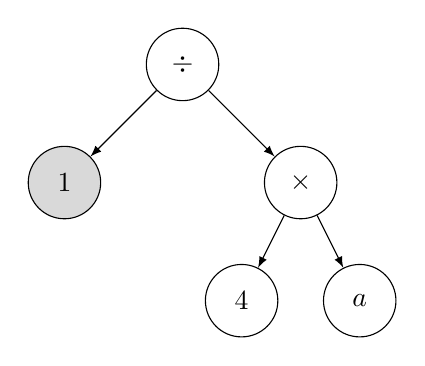
\begin{tikzpicture}[level/.style={sibling distance=30mm/#1},
                        every node/.style={draw, circle, minimum size=9.2mm},
                        edge from parent/.style={draw,-latex},
                        level distance=1.5cm]
                        
            \node (+) {$\div$}
                child { node[fill=gray!30] {$1$} }
                child { node {$\times$} 
                    child { node {$4$} }
                    child { node {$a$} }
                };
                
        \end{tikzpicture}}
    \end{subfigure}
    \begin{subfigure}{0.1\textwidth}
        \centering
        \adjustbox{valign=c}{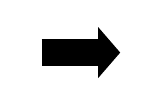
\begin{tikzpicture}
            \draw[-{Triangle[width=18pt,length=8pt]}, line width=10pt] (0,5) -- (1,5);
        \end{tikzpicture}}
    \end{subfigure}
    \begin{subfigure}{0.44\textwidth}
        \centering
        \adjustbox{valign=c}{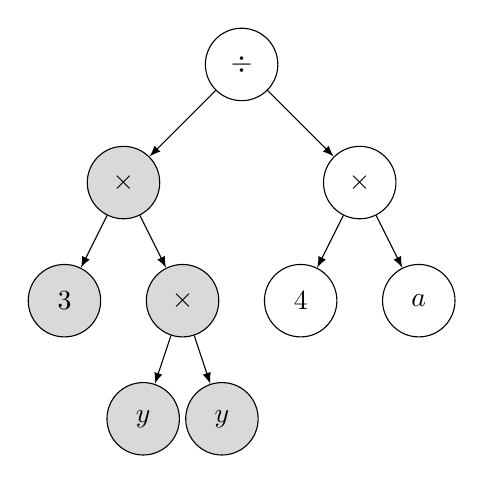
\begin{tikzpicture}[level/.style={sibling distance=30mm/#1},
                        every node/.style={draw, circle, minimum size=9.2mm},
                        edge from parent/.style={draw,-latex},
                        level distance=1.5cm]
            
            \node (+) {$\div$}
                child { node[fill=gray!30] {$\times$} 
                    child { node[fill=gray!30] {$3$} }
                    child { node[fill=gray!30] {$\times$} 
                        child { node[fill=gray!30] {$y$} }
                        child { node[fill=gray!30] {$y$} }
                    }
                }
                child { node {$\times$} 
                    child { node {$4$} }
                    child { node {$a$} }
                };
        \end{tikzpicture}}
    \end{subfigure}
    \caption{Indivíduo submetido a mutação, onde o terminal $1$ é substituído pela subárvore $\times(3,\times(y,y))$ aleatoriamente gerada.}
    \label{fig:mutacao-prog-genetica}
\end{figure}

\subsection{Outros métodos}

\begin{itemize}
    \item \textbf{Estratégias evolutivas (ES)} --- Introduzida por Rechenberg, Schwefel \textit{et al.} \cite{rechenberg:65, schwefel:95} nos anos 60, usa vetores de números reais como representação e tem como principal diferencial taxas de mutação variáveis. É aplicada principalmente em problemas de otimização numérica e combinatória;
    \item \textbf{Programação evolutiva (EP)} --- Trabalha submetendo máquinas de estado finito ao processo evolutivo, buscando autômatos capazes de reconhecer determinadas cadeias de caracteres, como formalizado por Fogel \textit{et al.} em 1966 \cite{fogel:66};
    \item \textbf{Algoritmos meméticos} --- Combinam elementos de algoritmos genéticos com processos de aprendizado cultural, empregando métodos evolutivos para encontrar novas soluções e refinamentos locais para melhorar as soluções encontradas \cite{chen:11}.
\end{itemize}

\chapter{Trabalhos Correlatos} \label{sec:trabalhos-correlatos}

Com a recente expansão da pesquisa em torno da inteligência artificial, uma variedade de trabalhos foram realizados buscando integrá-la à área de compiladores em geral e, consequentemente, aos problemas da alocação de registradores e geração de código \textit{spill}. Todavia, alguns obstáculos se fizeram presentes, como a indisponibilidade de \textit{datasets} para treinamento e a necessidade de exatidão nos algoritmos de geração de código, contrastando com a natureza aproximada das soluções produzidas por modelos de IA \cite{venkatakeerthy:23}.

Ainda assim, uma variedade de trabalhos apresentam resultados promissores ao utilizar técnicas de inteligência artificial para a obtenção de melhores heurísticas e promover uma minimização de \textit{spill code} mais eficiente. Este Capítulo tem por objetivo expor alguns desses trabalhos e apresentar um panorama do estado da arte das pesquisas recentes combinando IA e alocação de registradores.

\section{Minimização de \textit{Spill Code} com Algoritmos Evolutivos}

Em 2003, Stephenson \textit{et al.} \cite{amarasinghe:03} publicaram um trabalho que discute o uso de técnicas de inteligência artificial para obter automaticamente as heurísticas de várias etapas de otimização, incluindo a alocação de registradores. Os autores introduzem o conceito de \textit{``Meta Optimization''} ou metaotimização, em uma tradução livre, uma metodologia que emprega algoritmos evolutivos e auxilia os desenvolvedores de compiladores no trabalhoso processo de ajuste fino das heurísticas que norteiam as de otimização de código.

Após analisar várias otimizações de compiladores, os autores constataram que muitas heurísticas têm um ponto focal: uma única função de prioridade ou custo que muitas vezes dita a eficácia de uma heurística. Uma função de prioridade leva em conta os fatores que afetam um determinado problema, e apresenta uma medida da importância relativa das opções disponíveis em um processo de otimização. Sendo assim, o \textit{Meta Optimization} consiste de um modelo de aprendizado que envolve programação genética para se obter boas heurísticas, representadas na forma de expressões aritméticas avaliáveis em tempo de compilação, através do processo evolutivo.

Na abordagem de Stephenson \textit{et al.} \cite{amarasinghe:03}, as melhores heurísticas foram obtidas através do processo de evolução, sendo elas representadas como árvores sintáticas de expressões aritméticas tais quais as mostradas na Figura \ref{fig:stephenson}. O algoritmo de alocação de registradores usado nos experimentos foi o de alocação prioritária, onde a prioridade representa o ganho de performance ao se manter um \textit{live range} em registradores, ao invés de se realizar \textit{spill}. 

As heurísticas seriam usadas para determinar essa prioridade, influenciando na qualidade do resultado final da alocação. As árvores eram compostas de funções primitivas, como operações aritméticas entre números reais, e terminais que incluiam constantes e parâmetros sobre o \textit{live range} tendo sua prioridade calculada, como número de usos, definições, execuções, dentre outros. 

\begin{figure}[hbt]
    \centering
    \includegraphics[width=\textwidth]{stephenson}
    \caption{Cromossomos das funções de prioridade, submetidas a operações de cruzamento e mutação. Extraído de Stephenson \textit{et al.} \cite{amarasinghe:03}.}
    \label{fig:stephenson}
\end{figure}

\begin{figure}[hbt]
    \centering
    \includegraphics[scale=1.4]{stephenson-resultados}
    \caption{O eixo horizontal mostra o número de gerações, enquanto o eixo vertical apresenta o aumento na velocidade de execução. Extraído de Stephenson \textit{et al} \cite{amarasinghe:03}.}
    \label{fig:stephenson-resultados}
\end{figure}

O \textit{fitness} das heurísticas foi avaliado usando-as para compilar um conjunto de \textit{benchmarks}, coletando o tempo de execução dos programas produzidos por cada heurística e calculando o ganho de velocidade em comparação à heurística prioritária original. Uma população de 400 heurísticas foi submetida ao processo evolutivo por 50 gerações, para o qual houve uma taxa de substituição geracional média de 22\% dos indivíduos. Foi aplicada uma taxa de mutação de 5\%, e o algoritmo de seleção empregado foi o de seleção por torneio, utilizando-se um torneio de tamanho 7 \cite{stephenson:06}.

Os experimentos realizados por Stephenson \textit{et al.} apresentaram um aumento médio de 11\% na velocidade de execução com as heurísticas especializadas obtidas pelo \textit{Meta Optimization}, isto é, treinando uma população para cada \textit{benchmark} de teste. Em experimentos buscando uma heurística de uso geral, utilizando diferentes \textit{benchmarks} para a mesma população, o aumento médio foi de 3\%, que, apesar de menor do que o obtido com as heurísticas especializadas, ainda se mostra significativo. A Figura \ref{fig:stephenson-resultados} mostra o \textit{plot} do nível de \textit{fitness} ao longo das gerações, para o treinamento das heurísticas especializadas e da heurística de uso geral, respectivamente.

Outros trabalhos, como os de Kri e Feeley (2004) \cite{kri:04}, Mahajan e Ali (2008) \cite{mahajan:08}, além de Topcuoglu \textit{et al.} (2007) \cite{topcuoglu:07}, realizam experimentos com alocadores inteiramente genéticos, onde o mapeamento dos registradores virtuais para os físicos é representado na forma de cromossomos. Uma alocação válida para o conjunto de variáveis é então obtida através de um processo evolutivo, ao invés dos algoritmos tradicionais.

\section{Coloração de Grafos via \textit{Deep Learning}} \label{sec:coloracao-deep-learning}

Em um trabalho de 2019, Lemos \textit{et al.} \cite{lemos:19} lidam com problema da coloração utilizando um modelo de rede neural em grafo (GNN), um tipo de rede neural capaz de representar informações extraídas dos nós de um grafo \cite{scarselli:09}. O modelo utiliza um sistema de memória que mantém representações multidimensionais das informações sobre os vértices, associados a um conjunto de cores, além de uma rede neural recorrente (RNN) que computa as atualizações no sistema. O processo envolve 32 iterações de troca de mensagens entre vértices adjacentes e entre vértices e cores, para que o modelo obtenha a viabilidade das colorações para cada vértice. Cada vértice então decide se o grafo de entrada permite uma coloração com $k$ cores.

O modelo foi treinado utilizando uma abordagem generativa. As instâncias de treinamento foram criadas tomando instâncias reais e modificando seu número cromático ao adicionar vértices no grafo; em seguida, ambas as instâncias eram adicionadas no conjunto de treinamento. O modelo atingiu 82\% de precisão para instâncias após entre 40 e 60 gerações de treinamento, e número de cores $k$ entre 3 e 7. Além disso, os autores observaram que o modelo treinado generaliza bem para valores de $k$ não vistos anteriormente e instâncias maiores.

Os pesquisadores discutem na publicação como o funcionamento interno do modelo influencia sua tomada de decisão. Eles afirmam que o modelo procura uma resposta positiva ao agrupar vértices de forma a aproximar aqueles que poderiam ter a mesma cor. Apesar de agrupar vértices adjacentes em uma proporção baixa, o modelo continua a fornecer respostas positivas. O número desejado de cores ($k$) é introduzido no modelo com representações iniciais aleatórias, evitando qualquer conhecimento prévio.

Eles propõem melhorias futuras, como a redução de conflitos dentro do próprio modelo como uma métrica de perda, mesmo com o aumento da complexidade temporal e espacial. Os autores destacam que seu trabalho evidencia como um modelo semelhante ao GNN pode ser ajustado para solucionar desafiadores problemas combinatórios, como a coloração de grafos, de maneira interpretável, gerando resultados precisos e construtivos.

Em 2020, Das \textit{et al.} \cite{das:20} publicaram um trabalho que também envolve a alocação via coloração de grafos empregando modelos de \textit{deep learning}, especificamente, o alocador utiliza uma abordagem híbrida, como os próprios autores assim o descreveram, dividida em duas etapas: uma consiste na coloração propriamente dita, feita por uma rede neural multicamadas, e a outra consiste de uma etapa de correção. Os autores buscaram encontrar novas heurísticas através do \textit{deep learning}, apresentando resultados comparáveis ou até melhores do que os dos alocadores convencionais por coloração de grafos.

A coloração do grafo de interferência é feita por uma rede neural recorrente (RNN) composta por várias camadas de LSTM, ou \textit{``long short-term memory''}. O LSTM é uma arquitetura de RNN que possui memória, sendo capaz de armazenar valores em intervalos arbitrários. Uma célula LSTM é formada por um conjunto de neurônios organizados em ``portas'' que controlam o fluxo de informação: uma porta \textit{input} para entrada, uma porta \textit{output} para saída e a porta \textit{forget}, que controla o esquecimento da informação. A Figura \ref{fig:lstm} ilustra a organização básica de uma célula LSTM.

\begin{figure}[hbt]
    \centering
    \includegraphics[width=.7\textwidth]{lstm}
    \caption{Célula de memória LSTM. Extraído de Yu \textit{et al.} \cite{yu:19}.}
    \label{fig:lstm}
\end{figure}

A porta \textit{input} decide quais partes das novas informações devem ser armazenadas no estado atual, usando um sistema semelhante ao da porta \textit{forget}. A porta \textit{output} controla qual parte das informações no estado atual devem ser usadas, atribuindo um valor de 0 a 1 à informação, considerando os estados anterior e atual. A porta \textit{forget} determina quais informações descartar do estado anterior, atribuindo um valor entre 0 e 1 ao estado anterior em comparação com a entrada atual. Um valor próximo a 1 significa manter a informação, enquanto um valor próximo a 0 significa descartá-la. A produção seletiva de informações relevantes do estado atual permite que a rede LSTM mantenha dependências úteis de longo prazo para fazer previsões, tanto nos passos de tempo atuais quanto nos futuros \cite{yu:19, das:20}.

Visando maximizar a performance, o modelo foi arquitetado possuindo três camadas de células LSTM, com os estados ocultos de uma camada sendo repassados às células da camada seguinte. Os dados submetidos à camada de entrada da rede neural são as adjacências de cada vértice do grafo, sendo uma lista de adjacências $\mathit{adj}(v_i)$ para cada vértice $v_i$, e é produzido como saída uma sequência de cores $\mathit{cor}(v_i)$, cada qual correspondente à coloração de um vértice do grafo de interferência. A Figura \ref{fig:das-modelo} esquematiza a organização do modelo.

\begin{figure}[hbt]
    \centering
    \adjustbox{width=\textwidth}{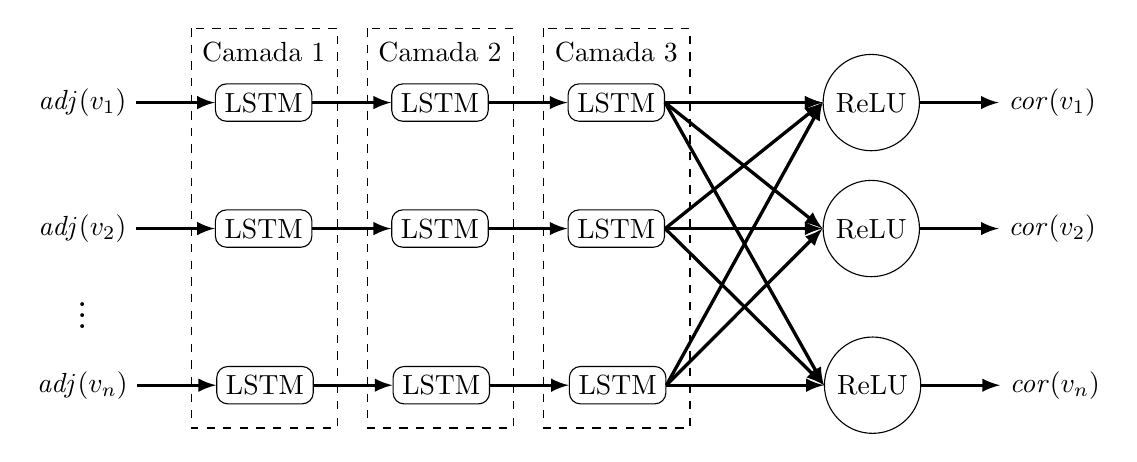
\begin{tikzpicture}[text centered]
        \node (adj_1) {$\mathit{adj}(v_1)$};
        \node[draw, rounded corners, right = of adj_1] (lstm_11) {LSTM};
        \node[draw, rounded corners, right = of lstm_11] (lstm_12) {LSTM};
        \node[draw, rounded corners, right = of lstm_12] (lstm_13) {LSTM};
        \node[draw, circle, right = 2cm of lstm_13] (output_1) {ReLU};
        \node[right = of output_1] (cor_1) {$\mathit{cor}(v_1)$};

        \draw[->, -latex, very thick] (adj_1) -- (lstm_11);
        \draw[->, -latex, very thick] (lstm_11) -- (lstm_12);
        \draw[->, -latex, very thick] (lstm_12) -- (lstm_13);
        \draw[->, -latex, very thick] (lstm_13) -- (output_1);
        \draw[->, -latex, very thick] (output_1) -- (cor_1);

        \node[below = of adj_1] (adj_2) {$\mathit{adj}(v_2)$};
        \node[draw, rounded corners, right = of adj_2] (lstm_21) {LSTM};
        \node[draw, rounded corners, right = of lstm_21] (lstm_22) {LSTM};
        \node[draw, rounded corners, right = of lstm_22] (lstm_23) {LSTM};
        \node[draw, circle, right = 2cm of lstm_23] (output_2) {ReLU};
        \node[right = of output_2] (cor_2) {$\mathit{cor}(v_2)$};

        \draw[->, -latex, very thick] (adj_2) -- (lstm_21);
        \draw[->, -latex, very thick] (lstm_21) -- (lstm_22);
        \draw[->, -latex, very thick] (lstm_22) -- (lstm_23);
        \draw[->, -latex, very thick] (lstm_23) -- (output_2);
        \draw[->, -latex, very thick] (output_2) -- (cor_2);

        \node[below = 3mm of adj_2] (dots) {\Large $\vdots$};

        \node[below = 3mm of dots] (adj_n) {$\mathit{adj}(v_n)$};
        \node[draw, rounded corners, right = of adj_n] (lstm_n1) {LSTM};
        \node[draw, rounded corners, right = of lstm_n1] (lstm_n2) {LSTM};
        \node[draw, rounded corners, right = of lstm_n2] (lstm_n3) {LSTM};
        \node[draw, circle, right = 2cm of lstm_n3] (output_n) {ReLU};
        \node[right = of output_n] (cor_n) {$\mathit{cor}(v_n)$};

        \draw[->, -latex, very thick] (adj_n) -- (lstm_n1);
        \draw[->, -latex, very thick] (lstm_n1) -- (lstm_n2);
        \draw[->, -latex, very thick] (lstm_n2) -- (lstm_n3);
        \draw[->, -latex, very thick] (lstm_n3) -- (output_n);
        \draw[->, -latex, very thick] (output_n) -- (cor_n);

        \draw[dashed] ([xshift=-3mm, yshift=7mm] lstm_11.north west) rectangle ([xshift=3mm, yshift=-3mm] lstm_n1.south east);
        \node at ([yshift=4mm] lstm_11.north) {Camada 1};

        \draw[dashed] ([xshift=-3mm, yshift=7mm] lstm_12.north west) rectangle ([xshift=3mm, yshift=-3mm] lstm_n2.south east);
        \node at ([yshift=4mm] lstm_12.north) {Camada 2};

        \draw[dashed] ([xshift=-3mm, yshift=7mm] lstm_13.north west) rectangle ([xshift=3mm, yshift=-3mm] lstm_n3.south east);
        \node at ([yshift=4mm] lstm_13.north) {Camada 3};

        \draw[->, -latex, very thick] (lstm_13.east) -- (output_1.west);
        \draw[->, -latex, very thick] (lstm_13.east) -- (output_2.west);
        \draw[->, -latex, very thick] (lstm_n3.east) -- (output_1.west);
        
        \draw[->, -latex, very thick] (lstm_23.east) -- (output_1.west);
        
        \draw[->, -latex, very thick] (lstm_n3.east) -- (output_2.west);
        \draw[->, -latex, very thick] (lstm_13.east) -- (output_n.west);
        \draw[->, -latex, very thick] (lstm_23.east) -- (output_n.west);
        
    \end{tikzpicture}
    }
    \caption{Esquema da rede neural de coloração. Adaptado de Das \textit{et al.} \cite{das:20}.}
    \label{fig:das-modelo}
\end{figure}

Todavia, em alguns casos o modelo realiza colorações inválidas, onde dois vértices adjacentes possuem a mesma cor. Sendo assim, a coloração produzida como resultado pela rede neural é submetida a uma fase subsequente de correções, onde as colorações inválidas são corrigidas. Para o treinamento, foram utilizados grafos de até 100 vértices gerados aleatoriamente usando a biblioteca \texttt{very nauty}, disponível em linguagem C. O modelo foi validado utilizando os \textit{benchmarks} da suíte do SPEC CPU\textsuperscript{\textregistered} 2017, e o desempenho do alocador foi comparado ao do alocador \texttt{greedy} do LLVM, um \textit{framework} em código aberto que contém várias ferramentas para o desenvolvimento de compiladores 
\cite{lattner:04}. 

O desempenho foi medido em relação ao número de registradores necessários para obter uma coloração válida sem necessidade de \textit{spill}. Sendo assim, o desempenho foi medido utilizando cinco \textit{benchmarks}. Em um deles (\texttt{508.namd\_r}), o modelo de \textit{deep learning} apresentou um resultado pior do que o alocador do LLVM, sendo 5\% pior. Nos demais (\texttt{505.mcf\_r}, \texttt{557.xz\_r}, \texttt{541.leela\_r} e \texttt{502.gcc\_r}), a rede neural apresentou um desempenho superior, de 2\%, 2,5\%, 7\% e 5\%, respectivamente.

\section{Alocação de Registradores com \textit{Reinforcement Learning}}

Em 2023, VenktaKeerthy \textit{et al.} \cite{venkatakeerthy:23} apresentaram uma aplicação que realiza a alocação de registradores empregando técnicas de \textit{reinforcemente learning} hierárquico e as ferramentas do LLVM. Eles abstraíram o problema de alocação dividindo-o em uma série de tarefas, cada uma sendo realizada por um agente inteligente, que se integram maneira hierárquica ao gerador de código do LLVM através de um \textit{framework} gRPC. A aplicação realiza a coloração de grafos de maneira não-iterativa, também sendo capaz de efetuar \textit{live range splitting}.

De maneira semelhante ao modelo de coloração de Lemos \textit{et al.} \cite{lemos:19} (\ref{sec:coloracao-deep-learning}), o modelo de inteligência artificial de VenktaKeerthy \textit{et al.} \cite{venkatakeerthy:23} representa o grafo de interferência codificando as instruções da representação intermediária de máquina (MIR) do LLVM, que então compõe o \textit{input} de uma \textit{gated graph neural network} (GGNN). A GGNN mantém uma visão do estado grafo de interferência, e a mantém atualizada conforme as alocações são realizadas realizando troca constante de informações entre os vértices. Além disso, elas permitem a anotação dos nós e arestas com base em seus tipos e propriedades, levando em consideração essas informações durante o aprendizado das representações.

O alocador foi denominado \textit{RL4ReAl} é composto de quatro agentes que se encarregam, cada um, de uma tarefa específica do processo de alocação de registradores. São eles, em ordem hierárquica:

\begin{enumerate}
    \item \textbf{\textit{Node selector}} --- agente encarregado de selecionar um vértice $v \in G$ levando em conta o custo de \textit{spill} e que, por consequência, determina a ordem de alocação. A política aprendida é considerada boa com base no resultado final da alocação. Portanto, a recompensa para este agente também é modelada com base nas recompensas dos agentes de nível inferior;

    \item \textbf{\textit{Task selector}} --- agente encarregado de decidir se uma variável específica será alocada para um registrador ou passará pelo processo de \textit{live range splitting}, levando em conta o número de registradores disponíveis, o número de interferências, seu tempo de vida e o custo de \textit{spill}. Sua recompensa é determinada com base na coloração da variável. Se a tarefa escolhida for o \textit{splitting}, então a recompensa é adiada até a decisão de coloração.

    \item \textbf{\textit{Splitter}} --- agente responsável por determinar os pontos de divisão dos \textit{live ranges} eleitos para \textit{splitting}. Para prever onde dividir os \textit{live ranges}, são levados em conta os custos de \textit{spil} em cada uso da variável, as distâncias entre usos sucessivos da variável e a codificação do vértice correspondente na GGNN. A recompensa é dada pela variação nas distâncias dos usos sucessivos da variável que sofreu \textit{split} e pela variação do número de interferências no grafo. Se a variação das distâncias de uso for maior do que a das interferências, a divisão é benéfica.

    \item \textbf{\textit{Coloring agent}} --- agente de nível inferior que aprende a selecionar uma cor válida para uma variável ou realizar \textit{spill} caso não haja registrador disponível. Sua recompensa é determinada pelo custo de \textit{spill} da variável: se o tempo de vida for colorido, o reforço é positivo; no entanto, se a variável for mapeada para memória, o reforço é negativo. Dessa forma, o agente aprende a priorizar a coloração de variáveis com custo mais elevado.
\end{enumerate}

Esses agentes constituem o modelo de \textit{reinforcement learning} implementado em linguagem Python, que interage com o otimizador do LLVM através de um \textit{framework} gRPC, que permite a realização de chamadas remotas entre programas diferentes. Dessa maneira, informações do grafo de interferência construído com as ferramentas do LLVM são enviadas para os agentes, e as decisões tomadas pelo \textit{Splitter} ou pelo \textit{Coloring agent} são devolvidas de modo a atualizar a representação do grafo presente no LLVM. A Figura \ref{fig:venktakeerthy} esquematiza a interação entre ambos os componentes através do gRPC.

\begin{figure}
    \centering
    \begin{tikzpicture}[align=center, minimum width=1.8cm, thick, minimum height=1.2cm, arrow/.style={->, -latex, thick}]
        \node[draw] (selector) {\textit{Node}\\\textit{selector}};
        \node[draw, below = 1cm of selector] (task) {\textit{Task}\\\textit{selector}};
        \node[draw, below left = 1cm and 0.25cm of task] (splitter) {\textit{Splitter}};
        \node[draw, below right = 1cm and 0.25cm of task] (coloring) {\textit{Coloring}\\\textit{agent}};
        
        \node[left = 2cm of selector] (ggnn) {\adjustbox{scale=0.4}{\begin{tikzpicture}[text centered, draw=black, node distance=1.5cm, >=Stealth, thick]
            
            % Camada de entrada
            \foreach \i in {1,...,4}
                \node[circle, draw, minimum size=0.75cm] (I-\i) at (0,-\i) {};
            
            % Camada oculta
            \foreach \h [count=\hi] in {1,...,4} % Ajuste o número de nós na camada oculta
                \node[circle, draw, minimum size=0.75cm, right = 1cm of I-\h] (H-\h) {};
    
            % Conexões entre camadas
            \foreach \i in {1,...,4}
                \foreach \h in {1,...,4}
                    \draw[-] (I-\i) -- (H-\h);
            \end{tikzpicture}}};
        \node[above = -4.8mm of ggnn] {GGNN};
        \node[left = 50mm of task, draw] (gRPC) {\textit{framework}\\gRPC};
        \node[left = 15mm of gRPC, draw] (grafo) {Grafo de\\interferência};
        \node[above = 1cm of grafo] (frontend) {\Large $\vdots$};
        \node[below = 1cm of grafo, draw] (gerador){Gerador de\\código};

        \draw[arrow] (frontend) -- (grafo);
        \draw[arrow] (grafo) -- (gerador);

        \draw[arrow] ([yshift=3mm] grafo.east) -- ([yshift=3mm] gRPC.west) % node[above] {Codificações}
        ;

        \draw[arrow] ([yshift=-3mm] gRPC.west) -- ([yshift=-3mm] grafo.east);

        \coordinate (z) at ([yshift=3mm] gRPC.east);
        \coordinate (w) at ([yshift=-3mm] gRPC.east);
        \coordinate (a) at (ggnn |- z);
        \coordinate (b) at (ggnn |- w);
        \coordinate (c) at ([yshift=-4mm] splitter.south);
        \coordinate (d) at ([yshift=-4mm] coloring.south);
        \coordinate (y) at (ggnn |- c);
        \draw[arrow] (a) -- (ggnn);
        \draw[arrow] (b) -- (w);
        \draw[-, thick] (z) -- (a);
        \draw[-, thick] (b) -- (y);
        \draw[-, thick] (c) -- (y);
        \draw[-, thick] (c) -- (splitter.south);
        \draw[-, thick] (c) -- (d);
        \draw[-, thick] (coloring.south) -- (d);

        \draw[arrow] (selector) -- (task);
        \draw[arrow] (task) -- (splitter.north east);
        \draw[arrow] (task) -- (coloring.north west);
        \draw[arrow] (ggnn) -- (selector);

        \coordinate (f) at ([xshift=3mm] grafo.east);
        \coordinate (g) at ([yshift=-7mm] gerador.south);
        \coordinate (h) at ([xshift=-3mm] grafo.west);
        % \coordinate (i) at ([yshift=3mm] frontend.north);
        \coordinate (m) at ([yshift=5mm] ggnn.north);
        \draw[dashed] (f |- g) rectangle (h |- m); 
        \coordinate (midpoint1) at ($(h |- m)!0.5!(f |- m)$);
        \node[above = 1mm of midpoint1] {LLVM};
        
        \coordinate (j) at ([xshift=3mm] coloring.east);
        \coordinate (k) at ([yshift=-7mm] coloring.south);
        \coordinate (l) at (ggnn.west);
        \draw[dashed] (j |- k) rectangle (l |- m); %node[above right] {\textit{Framework} de \textit{Reinforcement Learning}};
        \coordinate (midpoint2) at ($(l |- m)!0.5!(j |- m)$);
        \node[above = 1mm of midpoint2] {\textit{Framework} de \textit{Reinforcement Learning}};
    \end{tikzpicture}
    \caption{Esquema da interação entre o LLVM e o \textit{framework} de \textit{RL}. Adaptado de VenkataKeerthy \textit{et al.} \cite{venkatakeerthy:23}.}
    \label{fig:venktakeerthy}
\end{figure}

A tomada de decisões por parte dos agentes foi modelada como um processo de decisão de Markov, que representa processos de decisão sequenciais estocásticos em um sistema de estados, onde funções de custo e transição dependem apenas do estado atual do sistema e da ação atual \cite{puterman:90}. A Figura \ref{fig:markov} mostra um sistema de decisão de Markov, onde os nós do grafo representam os estados e as arestas representam as ações, cada uma possuindo, respectivamente, a recompensa pela tomada da ação e a probabilidade de se chegar ao estado seguinte.

\begin{figure}[hbt]
    \centering
    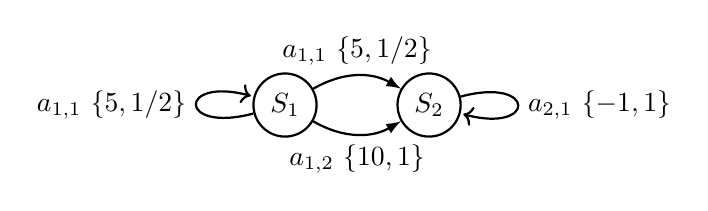
\begin{tikzpicture}[scale=2.0, thick, ->, -latex, thick]
        \node[draw, circle] (s1) {$S_1$};    
        \node[draw, circle, right = of s1] (s2) {$S_2$};

        \draw (s1) edge[bend left] node[above] {$a_{1,1}\ \{5,1/2\}$} (s2);
        \draw (s1) edge[bend right] node[below] {$a_{1,2}\ \{10,1\}$} (s2);
        \draw (s1) edge[loop left] node[left] {$a_{1,1}\ \{5,1/2\}$} (s1);
        \draw (s2) edge[loop right] node[right] {$a_{2,1}\ \{-1,1\}$} (s2);
    \end{tikzpicture}
    \caption{Esquema de uma instância de processo de decisão de Markov. Adaptado de Puterman \cite{puterman:90}.}
    \label{fig:markov}
\end{figure}

O treinamento foi realizado com 2 mil arquivos coletados aleatoriamente da suíte do SPEC CPU\textsuperscript{\textregistered} 2017 e da biblioteca \texttt{boost}, escrita em linguagem C++, utilizando uma estratégia de \textit{Proximal Policy Optimization} (PPO) para o ajuste das políticas de tomada de decisão dos agentes. Foram treinados dois modelos distintos, um empregando apenas recompensas locais e outro utilizando recompensas globais e locais simultaneamente.

O desempenho das alocações foi medido em termos do tempo de execução do programa resultante e número de acessos à memória, comparando o resultado de 18 \textit{benchmarks} dos SPEC CPU\textsuperscript{\textregistered} 2006 e 2017 utilizando-se o modelo de \textit{reinforcement learning} e os alocadores tradicionais do LLVM (\textit{basic}, \textit{greedy} e \textit{pbqp}). Os testes foram efetuados em duas máquinas: uma possuindo 32 GB de RAM, com um processador Intel Xeon SkyLake W2133 \textit{hexa-core} (arquitetura x86), e uma de 8 GB de RAM, ARM Cortex A72 \textit{dual-core} (arquitetura AArch64).

Em média, os resultados apresentados pelo \textit{RL4ReAl} são comparáveis ou ligeiramente melhores do que os dos alocadores do LLVM. Na arquitetura x86, o modelo de \textit{reinforcement learning} apresentou melhorias em tempo de execução de 1,59\% e 0,96\% em relação aos alocadores \textit{basic} e \textit{pbqp} respectivamente; em contrapartida, houve uma piora de 0,61\% com relação ao alocador \textit{greedy}. Em AArch64, o \textit{RL4ReAl} apresentou melhorias em comparação aos três alocadores do LLVM: 1,18\% sobre o \textit{basic}, 0,22\% sobre o \textit{pbqp} e 0,26\% em relação ao \textit{greedy}. O alocador de VenkataKeerthy \textit{et al.} também efetuou uma menor quantidade de \textit{reloads} por \textit{spill} em comparação aos alocadores do LLVM para ambas arquiteturas, demonstrando que os agentes de RL foram capazes de aprender uma boa política de escolha de variáveis para \textit{spill}.

De maneira análoga, Kim \textit{et al.} \cite{kim:22} propuseram a incorporação de técnicas de \textit{reinforcement learning} na alocação de registradores via PBQP. Os autores desenvolveram um alocador para sistemas embarcados voltados para teste de chips DRAM, empregando um modelo que resolve o PBQP utilizando heurísticas baseadas em processos estocásticos e aprimoradas através do aprendizado por reforço.

No trabalho de Kim \textit{et al.}, o grafo de resolução do PBQP é representado na forma de uma série de vetores numéricos, que são usados como entrada para uma rede convolucional em grafo (GCN). Então, o modelo realiza a alocação utilizando \textit{Monte Carlo search tree} (MCTS), uma técnica de busca em árvore baseada em processos estocásticos, muito empregada por agentes inteligentes destinados a jogos. O algoritmo da MCTS consiste em explorar uma árvore, que corresponde às possibilidades de jogadas ou ações em um sistema, com base em conhecimento prévio e realizando simulações a cada novo nó descoberto, de modo a adaptar a base de conhecimento com os dados das melhores jogadas para se atingir um resultado pré-determinado.

O treinamento do modelo foi conduzido utilizando-se grafos aleatórios gerados pelo modelo de Erdos-Rényi. Para a avaliação do desempenho do modelo, foram empregados 24 exemplos do \textit{suite} de testes do LLVM, e os resultados em tempo de execução foram comparados aos dos alocadores \textit{fast}, \textit{greedy} e \textit{pbqp} do LLVM; a opção \textit{fast}, que emprega alocação de registradores local, serviu como referência para os resultados obtidos. O modelo de RL de Kim \textit{et al.} apresentou resultados piores em apenas 2 \textit{benchmarks}, quando comparado com o alodador PBQP do LLVM.

\section{Outros trabalhos}

Alguns outros trabalhos abordam a aplicação de técnicas de \textit{machine learning} em problemas de otimização como a coloração de grafos de maneira geral, sem necessariamente ter relação com a alocação de registradores. Schuetz \textit{et al.} \cite{schuetz:22}, por exemplo, desenvolveram um método de coloração de grafos com redes neurais inspirado por princípios da física. Goudet \textit{et al.} \cite{goudet:22} propuseram um modelo combinando \textit{deep learning} e um \textit{framework} memético, um tipo de algoritmo evolutivo, executável em GPUs. 

Dodaro \textit{et al.} \cite{dodaro:22} treinaram um agente de \textit{deep learning} para gerar heurísticas visando resolver a coloração de grafos utilizando \textit{answer set programming} (ASP), um paradigma de inteligência artificial para a representação de bases de conhecimento e lógica. Musliu e Schwengerer \cite{musliu:13} identificaram 78 características dos grafos que podem indicar quais algoritmos se utilizar para realizar a coloração, e sugeriram técnicas de aprendizado de máquina para automaticamente classificar grafos e automaticamente escolher o melhor método de resolução.

No mais, a integração do aprendizado de máquina na alocação de registradores permanece ainda um horizonte relativamente inexplorado, com poucos trabalhos publicados na área. No entanto, esses seletos trabalhos já se mostram suficientemente promissores para motivar futuros esforços de pesquisa, visando desenvolver alocadores de registradores que empregam \textit{machine learning}.

\chapter{Proposta de Alocador de Registradores treinado com Programação Genética}

Inspirado pela implementação de Stephenson \cite{amarasinghe:03, stephenson:06}, este trabalho se propõe a implementar um alocador de registradores que faça uso de heurísticas obtidas através de algoritmos evolutivos. Mais especificamente, almeja-se reproduzir, mesmo que parcialmente, os resultados obtidos por Stephenson, que empregou programação genética no treinamento de heurísticas para seu alocador de registradores prioritário.

Stephenson \cite{amarasinghe:03, stephenson:06} demonstrou que a computação evolutiva é um boa abordagem de inteligência artificial para ser aplicada no desenvolvimento de compiladores. O treinamento através do processo evolutivo se mostrou capaz de encontrar eficientes heurísticas de uso específico e geral. Em particular, o trabalho de Stephenson mostra como os algoritmos evolutivos podem oferecer soluções quando não há disponibilidade de grandes conjuntos de dados e as relações entre as variáveis do problema são pouco compreendidas.

O trabalho de Bernstein \cite{bernstein:89} também demonstra como diferentes programas se beneficiam da utilização de heurísticas distintas, havendo espaço para uma otimização mais individual e específica que leva em conta as características do código. Essa constatação também motiva uma abordagem que busca o ajuste fino de determinadas heurísticas para cada categoria de programa. Sendo assim, neste trabalho as heurísticas de Bernstein serão utilizadas como parâmetro para avaliar as modificações feitas no compilador.

O LLVM é uma coleção de módulos e ferramentas de compilação utilizada por desenvolvedores de compiladores devido à sua versatilidade e modularidade. Seu funcionamento se baseia no uso de uma representação intermediária (IR) própria, mostrada na Figura \ref{fig:llvm-exemplo}, que funciona como uma linguagem de montagem abstrata. Ela é utilizada pelo \textit{back-end} LLVM para realizar otimizações e gerar código para uma variedade de arquiteturas-alvo \cite{llvm:01, lattner:02, lattner:04}. 

O \textit{framework} do LLVM provê ferramentas para manipulação da representação intermediária e geração de código, além de \textit{front-ends} que compilam de linguagem de alto nível para IR, como o compilador C/C++ Clang. Uma vez possuindo a IR de um programa, código executável pode ser gerado de maneira autônoma através do \textit{back-end} do LLVM \cite{llvm:01}. Por isso, o LLVM será utilizado para implementar as técnicas propostas e obter resultados experimentais.

\begin{figure}[ht]
    \centering
    \begin{lstlisting}[language=llvm, frame=single]
target triple = "x86_64-pc-linux-gnu"

@.str = private unnamed_addr constant [15 x i8] c"Hello, World!\0A\00", align 1

; Function Attrs: noinline nounwind optnone sspstrong uwtable
define dso_local i32 @main(i32 noundef %0, ptr noundef %1) #0 {
  %3 = alloca i32, align 4
  %4 = alloca i32, align 4
  %5 = alloca ptr, align 8
  store i32 0, ptr %3, align 4
  store i32 %0, ptr %4, align 4
  store ptr %1, ptr %5, align 8
  %6 = call i32 (ptr, ...) @printf(ptr noundef @.str)
  ret i32 0
}

declare i32 @printf(ptr noundef, ...) #1
    \end{lstlisting}
    \caption{Exemplo de representação intermediária (IR) do LLVM para um programa do tipo ``\textit{Hello, World!}''. Os números precedidos por ``\texttt{\%}'' são registradores virtuais.}
    \label{fig:llvm-exemplo}
\end{figure}

Para a implementação do modelo de treinamento utilizando algoritmos evolutivos a biblioteca DEAP \cite{fortin:12}, em Python, mostra-se útil ao prover uma gama de variedades de algoritmos evolutivos, como a programação genética, além de ferramentas para coleta de estatísticas e paralelização de execução. Será implementado um modelo de programação genética que irá manipular uma população de heurísticas candidatas, que terão seu \textit{fitness} avaliado inserindo-as no compilador modificado e medindo o tempo de execução dos programas gerados. O código será portado para um ambiente de experimentos onde a execução ocorrerá de maneira dedicada.

Como material de treinamento e validação, propõe-se a utilização dos arquivos-fonte dos \textit{benchmarks} do SPEC CPU\textsuperscript{\textregistered} 2017. 
O SPEC traz amostras de \textit{software} real utilizado em pesquisa acadêmica e produção, junto a ferramentas para coleta de métricas de execução e avaliação de performance. Vários desses programas realizam tarefas de computação intensiva, como simulações de sistemas complexos e compressão de dados, que produzem grande pressão sobre os registradores do ambiente de execução \cite{speccpu:01}. 
Por ser um padrão da indústria e pelas características dos programas de sua coletânea de \textit{benchmarks}, o SPEC foi escolhido para a realização de experimentos neste trabalho.

Os detalhes das técnicas utilizadas e decisões de implementação serão explicados no Capítulo \ref{cap:ambiente-de-experimentos}. Os resultados obtidos a partir dos experimentos serão discutidos no Capítulo \ref{cap:resultados}.

\chapter{Implementação e Ambiente de Experimentos} \label{cap:ambiente-de-experimentos}

\section{Compilador LLVM Modificado}

Na etapa de alocação de registradores, o LLVM possui quatro implementações distintas de alocadores: \texttt{fast}, \texttt{basic}, \texttt{greedy} e \texttt{pbqp}. Dos quatro, \texttt{fast}, \texttt{basic} e \texttt{greedy} realizam alocação via \textit{linear scan}, enquanto \texttt{pbqp} é um alocador experimental que utiliza a abordagem via PBQP. O alocador \texttt{fast} realiza a forma mais simples de \textit{linear scan}, percorrendo os registradores virtuais de maneira sequencial localmente nos blocos básicos, e inserindo \textit{spill code} somente no final dos blocos \cite{xavier:12}, enquanto o \texttt{pbqp} utiliza um método de alocação muito diferente dos demais. Por isso, neste trabalho o enfoque maior será nos alocadores de \textit{linear scan} \texttt{fast} e \texttt{greedy}. 

O alocador \texttt{basic} implementa uma extensão do método de \textit{linear scan} de Poletto e Sarkar \cite{poletto:99}, onde os registradores são alocados em um único passe pelo código e os \textit{live intervals} são percorridos em uma ordem predeterminada. No entanto, ao invés de um percurso linear ou em pós-ordem pelo grafo de controle de fluxo, como em implementações tradicionais, o alocador \texttt{basic} segue uma ordem prioritária. Cada registrador virtual tem seu peso de \textit{spill} calculado em um passe anterior, e esse peso é usado como valor de prioridade durante a alocação \cite{xavier:12}. % Fórmula cálculo pesos de spill

O alocador \texttt{greedy} é semelhante ao \texttt{basic}, funcionando com um \textit{linear scan} prioritário. No entanto, o critério de prioridade adotado pelo alocador \texttt{greedy} é o tamanho dos \textit{live intervals}. A utilização do peso, que representa a densidade de usos normalizada em relação ao tamanho da variável, promove a alocação dos menores intervalos vivos primeiro. Isso comumente causa o \textit{spill} de grandes intervalos, justificando a mudança na heurística usada. Além disso, o alocador \texttt{greedy} utiliza técnicas mais sofisticadas para minimizar a geração de \textit{spill code}, como o \textit{live range splitting} antes da alocação e a possibilidade de desalocar registradores físicos \textit{on the fly} (\textit{eviction}) \cite{xavier:12}.

Em ambos \texttt{basic} e \texttt{greedy}, a lista de intervalos é armazenada como uma fila de prioridade, que usa a implementação disponibilizada pela biblioteca padrão do C++. Sendo assim, o código-fonte foi modificado para que a fila de prioridade use como valor de prioridade o resultado de uma expressão, avaliada em tempo de compilação e recebida como argumento na chamada do compilador através da linha de comando. Essa expressão é a forma textual das heurísticas candidatas, que podem ser livremente alteradas conforme a necessidade.

\begin{figure}[htb]
    \centering
    \begin{tabular}{c c}
        \texttt{add(div(10, x), mul(sub(x, 3), y)} & \texttt{tern(b, 2, mul(sub(2, 0.4), 2))} \\
        \vspace{1cm}
        \adjustbox{scale=0.9}{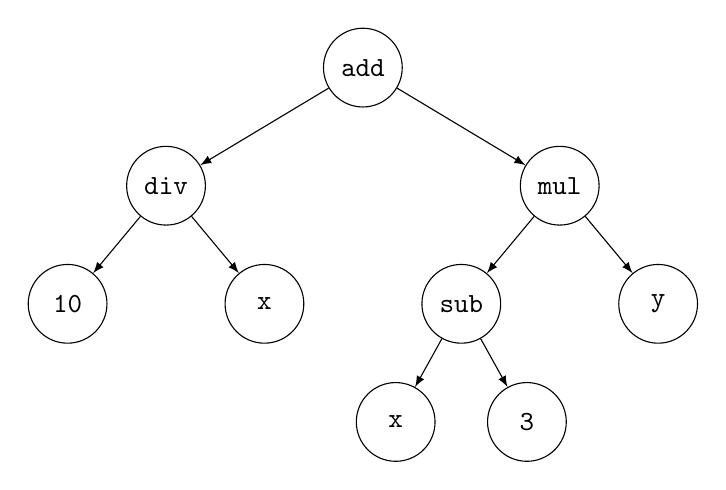
\begin{tikzpicture}[level/.style={sibling distance=50mm/#1},
                            every node/.style={draw, circle, minimum size=10mm},
                            edge from parent/.style={draw,-latex},
                            level distance=1.5cm]
            \node {\texttt{add}}
                child { node {\texttt{div}}
                    child { node {\texttt{10}} }
                    child { node {\texttt{x}} }
                }
                child { node {\texttt{mul}} 
                    child { node {\texttt{sub} }
                        child { node {\texttt{x}} }
                        child { node {\texttt{3}} }
                    }
                    child { node {\texttt{y}} }
                };
        \end{tikzpicture}} & \adjustbox{scale=0.9}{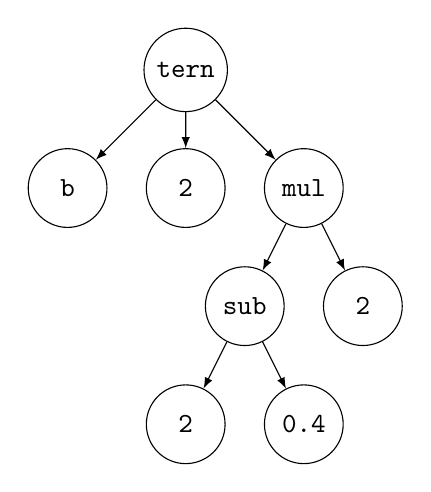
\begin{tikzpicture}[level1/.style={sibling distance=20mm/#1},
         level2/.style={sibling distance=25mm/#1},
         level3/.style={sibling distance=25mm/#1},
                            every node/.style={draw, circle, minimum size=10mm},
                            edge from parent/.style={draw,-latex},
                            level distance=1.5cm]
            \node {\texttt{tern}}
                child { node {\texttt{b}} }
                child { node {\texttt{2}} }
                child { node {\texttt{mul}} 
                    child { node {\texttt{sub}}
                        child { node {\texttt{2}} }
                        child { node {\texttt{0.4}} }
                    }
                    child { node {\texttt{2}} }
                };
        \end{tikzpicture}}
    \end{tabular}
    \caption{Exemplos de expressões no formato aceito pelo \textit{parser} de funções heurísticas embutido no LLVM, e suas respectivas representações em árvore.}
    \label{fig:expressoes}
\end{figure}

A Figura \ref{fig:expressoes} mostra o formato textual das expressões aceitas pelo compilador modificado junto às respectivas representações em árvore. Esse formato é o mesmo utilizado pela biblioteca DEAP para a manipulação dos cromossomos no algoritmo de programação genética. Nesta implementação, foi utilizado uma variante fortemente tipada de programação genética. Sendo assim, as expressões estão restritas às combinações válidas de acordo com o tipo de retorno de cada primitiva ou terminal, tal que os símbolos das árvores sintáticas podem possuir valor real ($R$) ou booleano ($B$). 

As primitivas reconhecidas pelo compilador incluem operações de retorno real, como as listadas na Tabela \ref{tab:primitivas-reais}, ou operações lógicas e de comparação, apresentadas na Tabela \ref{tab:primitivas-booleanas}. Os símbolos terminais incluem constantes numéricas de valor real ou booleano, além de um conjunto de variáveis cujo valor é obtido através das análises de código do LLVM. 

\begin{table}[htb]
    \centering
    \begin{tabular}{cc}
        \hline
        \textbf{Representação} & \textbf{Operação} \\
        \hline
        $\texttt{add(R}_1\texttt{, R}_2\texttt{)}$ & $R_1 + R_2$ \\
        $\texttt{sub(R}_1\texttt{, R}_2\texttt{)}$ & $R_1 - R_2$ \\
        $\texttt{mul(R}_1\texttt{, R}_2\texttt{)}$ & $R_1 \times R_2$ \\
        $\texttt{div(R}_1\texttt{, R}_2\texttt{)}$ & $R_1 \div R_2$ \\
        $\texttt{pow(R}_1\texttt{, R}_2\texttt{)}$ & $R_1^{R_2}$ \\
        $\texttt{sqrt(R}_1\texttt{)}$ & $\sqrt{R_1}$ \\
        $\texttt{tern(B}_1\texttt{, }\texttt{R}_1\texttt{, }\texttt{R}_2\texttt{)}$ & $\begin{cases}
             R_1, & \text{se } B_1 \\
             R_2, & \text{caso contrário}
         \end{cases}$ \\
        \hline
    \end{tabular}
    \caption{Representação textual das primitivas de retorno real reconhecidas pelo compilador, junto às respectivas definições matemáticas, nas quais $R$ são valores reais e $B$ são valores lógicos.}
    \label{tab:primitivas-reais}
\end{table}

\begin{table}[htb]
    \centering
    \begin{tabular}{cc}
        \hline
        \textbf{Representação} & \textbf{Operação} \\
        \hline
        $\texttt{and(B}_1\texttt{, B}_2\texttt{)}$ & $B_1 \land B_2$ \\
        $\texttt{or(B}_1\texttt{, B}_2\texttt{)}$ & $B_1 \lor B_2$ \\
        $\texttt{not(B}_1\texttt{)}$ & $\lnot B_1$ \\
        $\texttt{lt(R}_1\texttt{, R}_2\texttt{)}$ & $R_1 < R_2$ \\
        $\texttt{gt(R}_1\texttt{, R}_2\texttt{)}$ & $R_1 > R_2$ \\
        $\texttt{eq(R}_1\texttt{, R}_2\texttt{)}$ & $R_1 = R_2$ \\
        \hline
    \end{tabular}
    \caption{Representação textual das primitivas de retorno booleano reconhecidas pelo compilador, junto às respectivas definições matemáticas, nas quais $R$ são valores reais e $B$ são valores lógicos.}
    \label{tab:primitivas-booleanas}
\end{table}

% Os símbolos terminais incluem constantes numéricas de valor real ou booleano, além de um conjunto de variáveis cujo valor é obtido através das análises de código do LLVM. 
As variáveis terminais contém informações sobre os registradores virtuais e seus respectivos \textit{live intervals} associados, constituindo os parâmetros que produzem o espaço de soluções investigado pelo algoritmo evolutivo. A escolha das variáveis foi inspirada pela implementação de Stephenson \cite{stephenson:06} e pautada pelas estatísticas disponibilizadas pelo LLVM. As variáveis de retorno real são listadas na Tabela \ref{tab:terminais-reais}, enquanto as de retorno booleano na Tabela \ref{tab:terminais-booleanos}.

\begin{table}[htb]
    \centering
    \begin{tabular}{cp{11cm}}
        \hline
        \textbf{Variável} & \textbf{Parâmetro} \\
        \hline \hline
        \texttt{original} & Heurística original do alocador selecionado \\
        \hline
        \texttt{cost} & Custo de \textit{spill} de Chaitin \cite{chaitin:82} e Bernstein \cite{bernstein:89} \\
        \hline
        \texttt{degree} & Número de interferências do registrador virtual \\
        \hline
        \texttt{area} & Área do registrador virtual de Bernstein \cite{bernstein:89} \\
        \hline
        \texttt{instructions} & Número de instruções onde o registrador virtual é vivo \\
        \hline
        \texttt{uses} & Número de usos do registrador virtual \\
        \hline
        \texttt{defs} & Número de definições do registrador virtual \\
        \hline
        \texttt{calls} & Número de chamadas de função onde o registrador virtual é vivo \\
        \hline
        \texttt{refs} & Número de referências à endereços de memória onde o registrador virtual é vivo \\
        \hline
        \texttt{moves} & Número de \textit{moves} do registrador virtual \\
        \hline
        \texttt{averageFreq} & Frequência média de execução do registrador virtual \\
        \hline
        \texttt{numValues} & Número de valores no intervalo associado ao registrador virtual \\
        \hline
        \texttt{size} & Tamanho do intervalo associado ao registrador virtual \\
        \hline
        \texttt{numBlocks} & Número de blocos básicos onde o registrador virtual é vivo \\
        \hline
    \end{tabular}
    \caption{Variáveis contendo informações sobre os registradores virtuais de retorno real.}
    \label{tab:terminais-reais}
\end{table}

\begin{table}[htb]
    \centering
    \begin{tabular}{cp{11cm}}
        \hline
        \textbf{Variável} & \textbf{Parâmetro} \\
        \hline
        \hline
        \texttt{isSpillable} & Se o intervalo associado ao registrador virtual pode sofrer \textit{spill} \\
        \hline
        \texttt{hasAtLeastOneValue} & Se o intervalo associado ao registrador virtual possui ao menos um valor ao longo do programa \\
        \hline
        \texttt{isTerminator} & Se o intervalo associado ao registrador virtual se encontra no conjunto de saída de algum bloco básico \\
        \hline
    \end{tabular}
    \caption{Variáveis contendo informações sobre os registradores virtuais de retorno booleano.}
    \label{tab:terminais-booleanos}
\end{table}

\section{Modelo de Programação Genética}

A cada geração do modelo de programação genética, os cromossomos da população são convertidos para a sua forma textual e inseridos no compilador, servindo como funções heurísticas para compilar um \textit{benchmark} de treinamento. Então, é medido o tempo de execução dos executáveis gerados por cada cromossomo, e esse tempo é usado como o valor de \textit{fitness}. A variação escolhida de algoritmo evolutivo foi modificada para realizar uma minimização do \textit{fitness}, ao invés da maximização tradicional, para que sejam encontradas heurísticas que reduzam o tempo de execução.

A escolha dos parâmetros populacionais para o algoritmo de programação genética também se baseou nos experimentos de Stephenson, mas foi influenciada pelas limitações do ambiente de testes. A coleta do tempo de execução para cada heurística se mostrou um processo demorado e os recursos para efetuar um grande número de medições em paralelo, acelerando a execução do algoritmo, não estavam disponíveis. Portanto, foi definido um tamanho populacional de 100 indivíduos e o processo evolutivo foi efetuado por 30 gerações, valores inferiores aos usados por Stephenson \cite{amarasinghe:03, stephenson:06}. 

A probabilidade de cruzamento foi mantida em 90\%, aplicando recombinação de subárvores em um único ponto aleatoriamente escolhido em ambos os indivíduos. A mutação foi realizada com uma probabilidade de 10\%, também em um único ponto aleatório, inserindo novas expressões no lugar da subárvore com raiz no ponto de mutação. O algoritmo de variação, provido pela biblioteca, aplica exclusivamente um dos dois métodos por indivíduo, nunca ambos.

A seleção foi realizada de maneira probabilística através do método de seleção por torneio, com torneio de tamanho 7 efetuado em uma única rodada. A cada geração, a seleção foi aplicada sobre o conjunto contendo tanto os indivíduos ancestrais quanto os descendentes, tal como na estratégia evolutiva $(\mu + \lambda)$. Esse tipo de seleção propicia um grau considerável de elitismo, pois indivíduos aptos tem uma alta probabilidade de se manterem na população, mas ao mesmo tempo permite que a variabilidade genética se mantenha alta por mais iterações devido à seleção estocástica. 

\begin{table}[htb]
    \centering
    \begin{tabular}{cc}
        \hline
        \textbf{Parâmetro} & \textbf{Valor} \\
        \hline
        População & 100 \\
        % \hline
        Gerações & 30 \\
        % \hline
        Estratégia & $(\mu + \lambda)$ \\
        % \hline
        $\mu$ & 100 \\
        % \hline
        $\lambda$ & 100 \\
        % \hline
        Seleção & Torneio, $n = 7$ \\
        % \hline
        $P_\textit{cruzamento}$ & 90\% \\
        % \hline
        $P_\textit{mutação}$ & 10\% \\
        \hline
    \end{tabular}
    \caption{Parâmetros de execução do modelo de programação genética.}
    \label{tab:parametros-prog-genetica}
\end{table}

Também foi utilizado um \textit{hall-of-fame}, uma estrutura para armazenar o melhor indivíduo encontrado ao longo de todo o processo evolutivo, onde a melhor solução estaria armazenada ao final do treinamento. A Tabela \ref{tab:parametros-prog-genetica} sumariza os parâmetros de execução do modelo de programação genética utilizado. Também foi aplicado ao algoritmo um limite de altura de 17 níveis para as árvores correspondentes aos cromossomos pois, na programação genética, os cromossomos tendem se tornar excessivamente grandes.

\section{\textit{Benchmarks} de Treinamento e Ambiente de Execução}

Para mensurar os efeitos das modificações no compilador e o desempenho das heurísticas candidatas foram utilizados os programas da coletânea do SPEC CPU\textsuperscript{\textregistered} 2017. A \textit{suite} do SPEC inclui programas das mais variadas aplicações na computação científica e de produção, escritos em linguagem C, C++ e Fortran. Na realização dos testes, os arquivos foram compilados para a representação intermediária do LLVM através dos compiladores Clang, de C/C++, e Flang, de Fortran.

Dos 43 \textit{benchmarks}, 39 compilaram com sucesso. Alguns programas que possuem trechos de código Fortran não foram compilados corretamente pelo Flang, que ainda é um compilador experimental e em desenvolvimento ativo. Ainda assim, o Flang foi capaz de gerar executáveis válidos para os outros \textit{benchmarks} em Fortran. Os arquivos foram compilados usando o perfil de otimização \textit{peak} do SPEC, que conta com \textit{flags} específicas, e o compilador \textit{back-end} do LLVM \texttt{llc} foi chamado com a \textit{flag} \texttt{-O3}. 

Em posse dos arquivos de IR, o \textit{back-end} modificado do LLVM foi acionado através do executável \texttt{llc} para produzir arquivos executáveis e coletar estatísticas sobre o código produzido usando as heurísticas candidatas. As heurísticas de Bernstein \cite{bernstein:89} foram usadas para verificar o impacto da alteração na heurística de prioridade sobre a geração de código \textit{spill}. Os arquivos do SPEC forma compilados para as arquiteturas x86-64 e AArch64 com as heurísticas de Bernstein, sendo coletados os totais de instruções de \texttt{store} e \texttt{load}.

\begin{table}[htb]
    \centering
    \begin{tabular}{cl}
        \hline
        \textbf{\textit{Benchmark}} & \textbf{Área de aplicação} \\
        \hline %\hline 
        \texttt{505.mcf\_r} & Planejamento de rota de veículos \\
        % \hline
        \texttt{508.namd\_r} & Simulação de sistemas biomoleculares \\
        % \hline
        \texttt{525.x264\_r} & \textit{Encoding} de vídeo \\
        % \hline
        \texttt{531.deepsjeng\_r} & IA para xadrez usando poda alfa-beta \\
        % \hline
        \texttt{541.leela\_r} & IA para \textit{Go} usando árvores de Monte Carlo \\
        \hline
    \end{tabular}
    \caption{Benchmarks selecionados para treinamento e validação do modelo de programação genética e suas respectivas aplicações \cite{speccpu:01}.}
    \label{tab:benchmarks}
\end{table}

Em seguida, foram aleatoriamente selecionados cinco \textit{benchmarks} para serem usados como elementos de treinamento e validação do modelo de programação genética. Os treinamentos foram realizados em uma máquina Linux x86-64, Intel Core\textsuperscript{\textregistered} i3-4170, 2 núcleos com 4GB RAM, durando aproximadamente uma semana por resultado. Cada indivíduo foi executado dez vezes e o valor do \textit{fitness} foi calculado como a média de tempo das execuções, sendo que as avaliações foram feitas dois a dois em paralelo. 

Para o treinamento foram usados os \textit{inputs} da \textit{workload} \texttt{train} do SPEC, por seu tempo de execução menor, enquanto a validação usou a \textit{workload} \texttt{ref}\footnote[1]{As \textit{workloads} diferem pelo tamanho e quantidade de computações desencadeadas pelos arquivos de entrada dos \textit{benchmarks}. A documentação oficial recomenda a utilização da \textit{workload} \texttt{ref} para a coleta de métricas, mas os inputs da \texttt{train} também podem ser apropriados se a duração dos experimentos for um limitador 
\cite{speccpu:01}.}. A Figura \ref{fig:esquema-algoritmo} esquematiza o funcionamentodo modelo de programação genética em integração com o LLVM, onde as heurísticas da população são usadas para compilar os arquivos-fonte e o tempo de execução dos programas é usado como \textit{fitness} do algoritmo evolutivo.

\begin{figure}[htb]
    \centering
    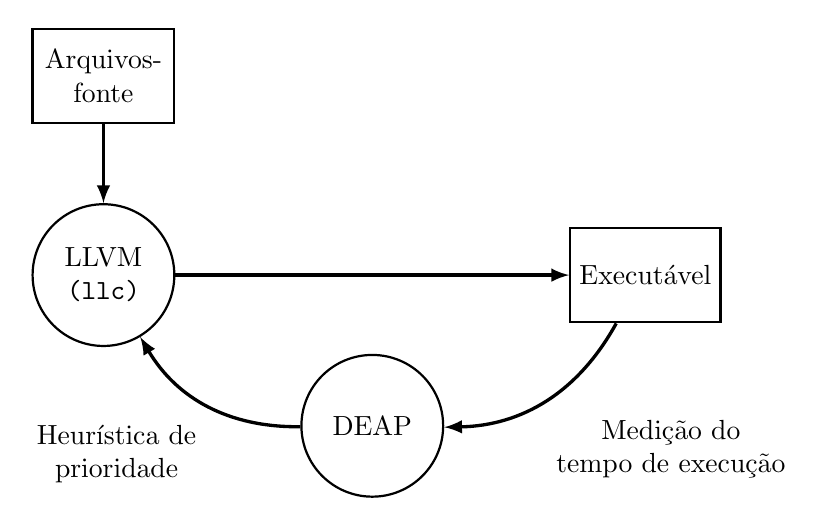
\begin{tikzpicture}[align=center, minimum width=1.8cm, thick, minimum height=1.2cm, arrow/.style={->, -latex, thick}]
        \node[draw, circle] (llc) {LLVM\\\texttt{(llc)}};
        \coordinate[right = 2.5cm of llc] (a) {};
        \node[draw, rectangle, right = 2.5cm of a] (exe) {Executável};
        \node[draw, circle, below = of a] (deap) {DEAP};
        \node[draw, rectangle, above = of llc] (src) {Arquivos-\\fonte};

        \draw[-latex, very thick] (src) to (llc) {};
        \draw[-latex, very thick] (llc) to (exe) {};
        \draw[-latex, very thick] (exe) edge[bend left] node[below right] {Medição do\\tempo de execução} (deap);
        \draw[-latex, very thick] (deap) edge[bend left] node[below left] {Heurística de\\prioridade} (llc);
    \end{tikzpicture}
    \caption{Esquematização do algoritmo de programação genética usado para se obter as melhores heurísticas.}
    \label{fig:esquema-algoritmo}
\end{figure}

Para coletar o número de acessos à memória em tempo de execução foi utilizado o Intel\textsuperscript{\textregistered} Pin, uma ferramenta de instrumentação e análise de código que funciona realizando a injeção de código executável em um programa em tempo de execução \cite{bach:10}. Código foi inserido nos \textit{benchmarks} compilados com as heurísticas obtidas de modo a contar as execuções de instruções de \textit{read} e \textit{write} em memória.

\chapter{Resultados} \label{cap:resultados}

Os resultados da compilação dos \textit{benchmarks} usando a heurística original e as três heurísticas de Bernstein, $h_1$, $h_2$ e $h_3$, são mostrados nas Tabelas \ref{tab:bernsteinbasic} (\texttt{basic}, x86-64), \ref{tab:bernsteingreedy} (\texttt{greedy}, x86-64), \ref{tab:bernsteinbasicaarch} (\texttt{basic}, AArch64) e \ref{tab:bernsteingreedyaarch} (\texttt{greedy}, AArch64). O compilador realizou a contagem de todas as instruções de acesso à memória após a alocação de registradores, e em ambas as arquiteturas x86-64 e AArch64 foram observadas diferenças significativas na quantidade de \texttt{stores} e \texttt{loads}, a depender da heurística escolhida. 

Nos \textit{benchmarks} compilados com o alocador \texttt{basic}, se sobressaiu a heurística $h_1$. Em 30 programas, na arquitetura x86-64, e 34, na arquitetura AArch64, a heurística $h_1$ foi a que produziu o menor total de instruções de acesso à memória no binário final. A heurística $h_2$ foi melhor em 5 e 4 programas, em x86-64 e AArch64 respectivamente; $h_3$ foi melhor em 3 programas e a heurística original em 1 programa, todos na arquitetura x86-64 somente.

\pgfplotstableread[row sep=\\,col sep=&] {
    benchmark       & original & h1 & h2 & h3 \\
    502.gcc\_r      & 106585 & 88030 & 88479 & 90350 \\
    510.parest\_r   & 180850 & 168553 & 174670 & 175385 \\
    526.blender\_r  & 144229 & 130365 & 133862 & 135200 \\
    538.imagick\_r  & 38827 & 33681 & 36589 & 35449 \\
    554.roms\_r     & 47998 & 40744 & 41928 & 41888 \\
} \bernsteinbasicspills

\pgfplotstableread[row sep=\\,col sep=&] {
    benchmark       & original & h1 & h2 & h3 \\
    502.gcc\_r & 54957 & 55800 & 59179 & 58722 \\
    510.parest\_r & 124011 & 122003 & 124447 & 123567 \\
    526.blender\_r & 86283 & 85744 & 89090 & 89190 \\
    538.imagick\_r & 23943 & 25088 & 26874 & 26966 \\
    554.roms\_r & 28972 & 29324 & 29106 & 29030 \\
} \bernsteingreedyspills

\pgfplotstableread[row sep=\\,col sep=&] {
    benchmark       & original & h1 & h2 & h3 \\
    basic (x86-64) & 34927,82 & 31646,58 & 32378,11 & 32634,18 \\
    greedy (x86-64) & 21564,61 & 21241,39 & 22178,95 & 22090,63 \\
    basic (AArch64) & 21651,29 & 18608,07 & 19218,79 & 19501,19 \\
    greedy (AArch64) & 12871,14 & 12929,45 & 13285,17 & 13321,90 \\
} \bernsteintotal

\begin{table}[htb]
    \centering
    \resizebox{\textwidth}{!}{
    \begin{tabular}{l|*{4}{>{\centering\arraybackslash}p{15.45mm}}|*{4}{>{\centering\arraybackslash}p{15.45mm}}}
        \hline
        \multirow{2}{*}{\textbf{\textit{Benchmark}}} 
        & \multicolumn{4}{c}{\#\texttt{store}} & \multicolumn{4}{c}{\#\texttt{load}} \\\cline{2-9}
                  & \textbf{Original} & $h_1$  & $h_2$ & $h_3$ & \textbf{Original} & $h_1$  & $h_2$ & $h_3$ \\
        \hline
        \texttt{502.gcc\_r} & 24378 & 21934 & 22664 & 23469 & 82207 & 66096 & 65815 & 66881 \\
        \texttt{510.parest\_r} & 55025 & 52288 & 54419 & 54933 & 125825 & 116265 & 120251 & 120452 \\
        \texttt{526.blender\_r} & 38528 & 36498 & 37462 & 37916 & 105701 & 93867 & 96400 & 97284 \\
        \texttt{538.imagick\_r} & 9094 & 8606 & 8588 & 8702 & 29733 & 25075 & 28001 & 26747 \\
        \texttt{554.roms\_r} & 15153 & 12220 & 12433 & 12455 & 32845 & 28524 & 29495 & 29433 \\\hline%\hline
        Média (geral) & 9838,5 & 8943,29 & 9094,26 & 9219,21 & 25089,32 & 22703,29 & 23283,84 & 23414,97 \\\hline
    \end{tabular}}
    \caption{Total de instruções de \texttt{store} e \texttt{load} contabilizadas no código resultante do processo de alocação de registradores, usando o alocador \texttt{basic} na arquitetura x86-64.}
    \label{tab:bernsteinbasic}
\end{table}

\begin{table}[htb]
    \centering
    \resizebox{\textwidth}{!}{
    \begin{tabular}{l|*{4}{>{\centering\arraybackslash}p{15.45mm}}|*{4}{>{\centering\arraybackslash}p{15.45mm}}}
        \hline
        \multirow{2}{*}{\textbf{\textit{Benchmark}}} 
        % & \multicolumn{2}{c}{\textbf{Original}} & \multicolumn{2}{c}{$h_1$} & \multicolumn{2}{c}{$h_2$} & \multicolumn{2}{c}{$h_3$} \\\cline{2-9}
        & \multicolumn{4}{c}{\#\texttt{store}} & \multicolumn{4}{c}{\#\texttt{load}} \\\cline{2-9}
                                   & \textbf{Original} & $h_1$  & $h_2$ & $h_3$ & \textbf{Original} & $h_1$  & $h_2$ & $h_3$ \\
        \hline
        502.gcc\_r & 17146 & 16924 & 17558 & 17236 & 37811 & 38876 & 41621 & 41486 \\
        510.parest\_r & 45231 & 45575 & 47246 & 46275 & 78780 & 76428 & 77201 & 77292 \\
        526.blender\_r & 31796 & 31583 & 31957 & 31908 & 54487 & 54161 & 57133 & 57282 \\
        538.imagick\_r & 6911 & 7163 & 7327 & 7455 & 17032 & 17925 & 19547 & 19511 \\
        554.roms\_r & 9868 & 9890 & 9845 & 9830 & 19104 & 19434 & 19261 & 19200 \\\hline
        Média (geral) & 7652,39 & 7482,82 & 7612,16 & 7554,97 & 13912,21 & 13758,58 & 14566,79 & 14535,66 \\\hline
    \end{tabular}}
    \caption{Total de instruções de \texttt{store} e \texttt{load} contabilizadas no código resultante do processo de alocação de registradores, usando o alocador \texttt{greedy} na arquitetura x86-64.}
    \label{tab:bernsteingreedy}
\end{table}

\begin{table}[htb]
    \centering
    \resizebox{\textwidth}{!}{
    \begin{tabular}{l|*{4}{>{\centering\arraybackslash}p{15.45mm}}|*{4}{>{\centering\arraybackslash}p{15.45mm}}}
        \hline
        \multirow{2}{*}{\textbf{\textit{Benchmark}}} 
        & \multicolumn{4}{c}{\#\texttt{store}} & \multicolumn{4}{c}{\#\texttt{load}} \\\cline{2-9}
                  & \textbf{Original} & $h_1$  & $h_2$ & $h_3$ & \textbf{Original} & $h_1$  & $h_2$ & $h_3$ \\
        \hline
        \texttt{502.gcc\_r} & 14116 & 11317 & 11899 & 12303 & 46639 & 34896 & 35095 & 36310 \\
        \texttt{510.parest\_r} & 51449 & 50350 & 51415 & 51976 & 131095 & 120668 & 124657 & 125809 \\
        \texttt{526.blender\_r} & 16328 & 14254 & 15011 & 15353 & 62622 & 48961 & 51867 & 52866 \\
        \texttt{538.imagick\_r} & 4035 & 3963 & 4139 & 4242 & 18550 & 16293 & 15496 & 15787 \\
        \texttt{554.roms\_r} & 7047 & 5538 & 5665 & 5794 & 31024 & 28435 & 29053 & 29445 \\\hline
        Média (geral) & 5144,43 & 4643,45 & 4805,57 & 4886,19 & 16506,86 & 13964,62 & 14413,21 & 14615 \\\hline
    \end{tabular}}
    \caption{Total de instruções de \texttt{store} e \texttt{load} contabilizadas no código resultante do processo de alocação de registradores, usando o alocador \texttt{basic} na arquitetura AArch64.}
    \label{tab:bernsteinbasicaarch}
\end{table}

\begin{table}[htb]
    \centering
    \resizebox{\textwidth}{!}{
    \begin{tabular}{l|*{4}{>{\centering\arraybackslash}p{15.45mm}}|*{4}{>{\centering\arraybackslash}p{15.45mm}}}
        \hline
        \multirow{2}{*}{\textbf{\textit{Benchmark}}} 
        % & \multicolumn{2}{c}{\textbf{Original}} & \multicolumn{2}{c}{$h_1$} & \multicolumn{2}{c}{$h_2$} & \multicolumn{2}{c}{$h_3$} \\\cline{2-9}
        & \multicolumn{4}{c}{\#\texttt{store}} & \multicolumn{4}{c}{\#\texttt{load}} \\\cline{2-9}
                                   & \textbf{Original} & $h_1$  & $h_2$ & $h_3$ & \textbf{Original} & $h_1$  & $h_2$ & $h_3$ \\
        \hline
        \texttt{502.gcc\_r} & 8184 & 7917 & 8112 & 7887 & 19149 & 19368 & 20583 & 20317 \\
        \texttt{510.parest\_r} & 48207 & 51005 & 52904 & 53072 & 89743 & 86056 & 88603 & 88115 \\
        \texttt{526.blender\_r} & 12458 & 12406 & 12535 & 12404 & 25641 & 25910 & 27293 & 27167 \\
        \texttt{538.imagick\_r} & 3023 & 2933 & 3203 & 3263 & 8915 & 9038 & 9793 & 11438 \\
        \texttt{554.roms\_r} & 5655 & 5627 & 5625 & 5603 & 18005 & 18612 & 19029 & 19347 \\\hline
        Média (geral) & 4159,48 & 4206,33 & 4277 & 4258,93 & 8711,67 & 8723,12 & 9008,17 & 9062,98 \\\hline
    \end{tabular}}
    \caption{Total de instruções de \texttt{store} e \texttt{load} contabilizadas no código resultante do processo de alocação de registradores, usando o alocador \texttt{greedy} na arquitetura AArch64.}
    \label{tab:bernsteingreedyaarch}
\end{table}

Já no caso do alocador \texttt{greedy}, constata-se que a disparidade entre as heurísticas, particularmente da original em relação às três heurísticas de Bernstein, é substancialmente menor. Na verdade, a heurística original foi a que obteve o melhor desempenho com o alocador \texttt{greedy}, se sobressaindo em 18 programas de x86-64 e 22 de AArch64. $h_1$ foi superior em 11 programas tanto de x86-64 quanto de AArch64; $h_2$ foi superior em 4 e 2, enquanto $h_3$ se sobressaiu em 6 e 3 programas de x86-64 e AArch64 respectivamente.

\begin{figure}[htb]
    \centering
    % \begin{tikzpicture}
    %     \begin{axis}[
    %             ybar,
    %             % ymax=250000,
    %             ylabel={$\#\texttt{store}+\#\texttt{load}$},
    %             symbolic x coords={502.gcc\_r,526.blender\_r,510.parest\_r,554.roms\_r,538.imagick\_r},
    %             xtick=data,
    %             tick label style={font=\ttfamily},
    %             nodes near coords,
    %             nodes near coords align={horizontal},
    %             nodes near coords style={font=\small, rotate=90, anchor=west},
    %             width=\textwidth, height=.5\textwidth,
    %             legend style={at={(0.5,-0.13)}, anchor=north},
    %             legend columns={4},
    %             legend image post style={scale=2},
    %             ]
                     
    %         \addplot +[black, fill=yellow, postaction={pattern=north east lines}] table[x=benchmark,y=original]{\bernsteinbasicspills};
    %         \addplot +[black, fill=cyan, postaction={pattern=fivepointed stars}] table[x=benchmark,y=h1]{\bernsteinbasicspills};
    %         \addplot +[black, fill=green, postaction={pattern=bricks}] table[x=benchmark,y=h2]{\bernsteinbasicspills};
    %         \addplot +[black, fill=magenta, postaction={pattern=checkerboard}] table[x=benchmark,y=h3]{\bernsteinbasicspills};
    %     \end{axis}
    % \end{tikzpicture}
    \begin{tikzpicture}
        \begin{axis}[
                ybar,
                % title={\texttt{greedy} (x86-64)},
                ymax=45000,
                ylabel={média de $\#\texttt{store}+\#\texttt{load}$},
                symbolic x coords={basic (x86-64), greedy (x86-64), basic (AArch64), greedy (AArch64)},
                xtick=data,
                tick label style={font=\ttfamily},
                nodes near coords,
                nodes near coords align={horizontal},
                nodes near coords style={font=\small, rotate=90, anchor=west},
                width=\textwidth, height=.5\textwidth,
                legend style={at={(0.5,-0.13)}, anchor=north},
                legend columns={4},
                legend image post style={scale=2},
                ]
                     
            \addplot +[black, fill=yellow, postaction={pattern=north east lines}] table[x=benchmark,y=original]{\bernsteintotal};
            \addplot +[black, fill=cyan, postaction={pattern=fivepointed stars}] table[x=benchmark,y=h1]{\bernsteintotal};
            \addplot +[black, fill=green, postaction={pattern=bricks}] table[x=benchmark,y=h2]{\bernsteintotal};
            \addplot +[black, fill=magenta, postaction={pattern=checkerboard}] table[x=benchmark,y=h3]{\bernsteintotal};
            
            \legend{Original, $h_1$, $h_2$, $h_3$}
        \end{axis}
    \end{tikzpicture}
    \caption{Comparativo da média de \textit{spill code} após alocação de registradores, entre alocadores e arquiteturas.}
    \label{fig:bernstein-stores-basic}
\end{figure}

Independente da arquitetura ou da heurística escolhida, o alocador \texttt{greedy} produziu menos \textit{spill code} para todos os \textit{benchmarks}, exceto pelo programa \texttt{519.lbm\_r}. Isso é um reflexo da implementação de técnicas mais sofisticadas de minimização de \textit{spill code} no alocador \texttt{greedy}, como o \textit{live range splitting} e a capacidade de se fazer \textit{spill} de um registrador físico já alocado (\textit{eviction}). A Figura \ref{fig:bernstein-stores-basic} apresenta uma comparação gráfica entre as médias \textit{spill code} por alocador e arquitetura.

Também nota-se que, por depender somente da heurística de prioridade para minimizar a inserção de \textit{spill code}, o alocador \texttt{basic} é mais sensível às alterações na função heurística. Entretanto, na maioria dos casos os programas gerados com o alocador \texttt{greedy} performam melhor \cite{xavier:12, venkatakeerthy:23}, e o \texttt{greedy} é a escolha padrão quando o nível máximo de otimização é habilitado no compilador. Por isso, os treinamentos com o algoritmo de programação genética se concentraram nele.

\pgfplotstableread[row sep=\\,col sep=&] {
    benchmark        & original  & heur      & speedup \\
    505.mcf\_r       & 406.08185 & 408.5062  & -0,59\% \\
    508.namd\_r      & 236.9738  & 239.6275  & -1,11\% \\
    525.x264\_r      & 198.1714  & 196.9088  & 0,64\%  \\
    531.deepsjeng\_r & 280.90245 & 274.1921  & 2,45\%  \\
    541.leela\_r	 & 427.58095 & 429.11035 & -0,36\% \\
} \runtimesdeepsjeng

O modelo de programação genético foi executado duas vezes, uma vez utilizando o \textit{benchmark} \texttt{531.deepsjeng\_r} e outra \texttt{508.namd\_r} como elementos de treinamento em cada execução, ao longo de 11 e 5 dias respectivamente. A Figura \ref{fig:fitness-prog-gen} mostra de maneira gráfica o \textit{fitness} --- melhora no tempo de execução em relação à geração inicial --- ao longo das iterações do algoritmo. 

Para o programa \texttt{531.deepsjeng\_r}, o modelo rapidamente encontrou um ótimo local por volta da 10ª geração e somente pequenos incrementos no tempo de execução foram obtidos até a geração 30, convergindo para um tempo de execução de aproximadamente 49 segundos com a \textit{workload} de treinamento. Ao final da execução foi encontrada a heurística mostrada à esquerda na Figura \ref{fig:melhor-heuristica-deepsjeng}.

\pgfplotstableread[row sep=\\, col sep=&] {
    gen & nevals & fit_dvp     & fit_max & fit_avg & fit_min & size_dvp & size_max & size_avg & size_min \\ 
    0   & 100    & 0.223599    & 50.437  & 49.7657 & 49.2405 & 2.02593  & 11       & 4.34     & 1        \\ 
    1   & 100    & 0.0992432   & 49.7447 & 49.4725 & 49.2405 & 1.75545  & 8        & 4.72     & 1        \\ 
    2   & 100    & 0.0661455   & 49.5059 & 49.377  & 49.2405 & 1.62899  & 8        & 4.92     & 2        \\ 
    3   & 100    & 0.0599056   & 49.4604 & 49.3094 & 49.2194 & 1.27949  & 7        & 5.23     & 2        \\ 
    4   & 100    & 0.0372331   & 49.3532 & 49.2516 & 49.192  & 1.12512  & 7        & 5.29     & 2        \\ 
    5   & 100    & 0.0357556   & 49.2826 & 49.2053 & 49.0903 & 1.23596  & 9        & 5.82     & 3        \\ 
    6   & 100    & 0.0449289   & 49.2405 & 49.1632 & 49.0903 & 1.51842  & 9        & 6.88     & 5        \\ 
    7   & 100    & 0.0410833   & 49.192  & 49.1171 & 49.062  & 1.42324  & 9        & 8.12     & 5        \\ 
    8   & 100    & 0.0140998   & 49.1763 & 49.0857 & 49.0611 & 0.198997 & 9        & 8.98     & 7        \\ 
    9   & 100    & 0.0197231   & 49.2213 & 49.0764 & 49.0611 & 0.198997 & 9        & 8.98     & 7        \\ 
    10  & 100    & 0.00649157  & 49.0903 & 49.0635 & 49.0611 & 0        & 9        & 9        & 9        \\ 
    11  & 100    & 0.00389263  & 49.0903 & 49.0619 & 49.0611 & 0        & 9        & 9        & 9        \\ 
    12  & 100    & 0.000213738 & 49.062  & 49.0612 & 49.0611 & 0        & 9        & 9        & 9        \\ 
    13  & 100    & 0.00211636  & 49.0611 & 49.0607 & 49.0503 & 0        & 9        & 9        & 9        \\ 
    14  & 100    & 0.0157005   & 49.2136 & 49.0613 & 49.0503 & 0.198997 & 11       & 9.02     & 9        \\ 
    15  & 100    & 0.0050783   & 49.0611 & 49.0575 & 49.0503 & 0        & 9        & 9        & 9        \\ 
    16  & 100    & 0.0332811   & 49.3127 & 49.0574 & 49.0503 & 0.223383 & 11       & 9.01     & 8        \\ 
    17  & 100    & 0.00192659  & 49.0611 & 49.0507 & 49.0503 & 0        & 9        & 9        & 9        \\ 
    18  & 100    & 0           & 49.0503 & 49.0503 & 49.0503 & 0        & 9        & 9        & 9        \\ 
    19  & 100    & 0.00912548  & 49.1339 & 49.0504 & 49.032  & 0        & 9        & 9        & 9        \\ 
    20  & 100    & 0.0217855   & 49.2537 & 49.0506 & 49.032  & 0.198997 & 9        & 8.98     & 7        \\ 
    21  & 100    & 0.0160376   & 49.1816 & 49.0459 & 49.032  & 0        & 9        & 9        & 9        \\ 
    22  & 100    & 0.00813075  & 49.0503 & 49.0371 & 49.032  & 0        & 9        & 9        & 9        \\ 
    23  & 100    & 0.0101851   & 49.1329 & 49.0332 & 49.032  & 0        & 9        & 9        & 9        \\ 
    24  & 100    & 0.0182182   & 49.2151 & 49.0338 & 49.032  & 0.198997 & 11       & 9.02     & 9        \\ 
    25  & 100    & 0           & 49.032  & 49.032  & 49.032  & 0        & 9        & 9        & 9        \\ 
    26  & 100    & 0           & 49.032  & 49.032  & 49.032  & 0        & 9        & 9        & 9        \\ 
    27  & 100    & 0.00841759  & 49.1166 & 49.0328 & 49.032  & 0        & 9        & 9        & 9        \\ 
    28  & 100    & 0           & 49.032  & 49.032  & 49.032  & 0        & 9        & 9        & 9        \\ 
    29  & 100    & 0.0391133   & 49.4153 & 49.0367 & 49.032  & 0.198997 & 11       & 9.02     & 9        \\
} \genprogdeepsjeng

\pgfplotstableread[row sep=\\, col sep=&] {
    gen & nevals & dvp & fit_max & fit_avg & fit_min & size_dvp & max & media & min \\
        0 & 100 & 0.233562 & 26.8872 & 26.2933 & 25.8027 & 2.20751 & 11 & 4.63 & 1 \\
        1 & 100 & 0.0914759 & 26.3184 & 26.0367 & 25.8027 & 2.04206 & 11 & 4.1 & 1 \\
        2 & 100 & 0.0542309 & 26.0655 & 25.9339 & 25.8027 & 2.27901 & 11 & 4.19 & 1 \\
        3 & 100 & 0.0390051 & 25.9754 & 25.8829 & 25.8027 & 2.42891 & 10 & 3.98 & 1 \\
        4 & 100 & 0.039036 & 26.0767 & 25.8432 & 25.7952 & 1.26317 & 10 & 3.38 & 3 \\
        5 & 100 & 0.0191684 & 25.8929 & 25.8126 & 25.7952 & 0.733212 & 5 & 3.32 & 3 \\
        6 & 100 & 0.0127907 & 25.9184 & 25.8013 & 25.7952 & 0.341174 & 5 & 3.06 & 3 \\
        7 & 100 & 0.00267729 & 25.8027 & 25.7967 & 25.7952 & 0 & 3 & 3 & 3 \\
        8 & 100 & 0.00505655 & 25.8444 & 25.796 & 25.7952 & 0 & 3 & 3 & 3 \\
        9 & 100 & 0.00416414 & 25.8369 & 25.7957 & 25.7952 & 0 & 3 & 3 & 3 \\
        10 & 100 & 3.55271e-15 & 25.7952 & 25.7952 & 25.7952 & 0 & 3 & 3 & 3 \\
        11 & 100 & 3.55271e-15 & 25.7952 & 25.7952 & 25.7952 & 0 & 3 & 3 & 3 \\
        12 & 100 & 0.00427845 & 25.8382 & 25.7956 & 25.7952 & 0 & 3 & 3 & 3 \\
        13 & 100 & 0.000915388 & 25.8044 & 25.7953 & 25.7952 & 0 & 3 & 3 & 3 \\
        14 & 100 & 0.0107658 & 25.9034 & 25.7963 & 25.7952 & 0 & 3 & 3 & 3 \\
        15 & 100 & 3.55271e-15 & 25.7952 & 25.7952 & 25.7952 & 0 & 3 & 3 & 3 \\
        16 & 100 & 3.55271e-15 & 25.7952 & 25.7952 & 25.7952 & 0 & 3 & 3 & 3 \\
        17 & 100 & 0.00460679 & 25.8415 & 25.7957 & 25.7952 & 0 & 3 & 3 & 3 \\
        18 & 100 & 0.006524 & 25.8418 & 25.7961 & 25.7952 & 0 & 3 & 3 & 3 \\
        19 & 100 & 0.011928 & 25.7952 & 25.7935 & 25.71 & 0.28 & 5 & 3.04 & 3 \\
        20 & 100 & 0.0244387 & 25.8569 & 25.7879 & 25.71 & 0.649923 & 5 & 3.24 & 3 \\
        21 & 100 & 0.0345501 & 25.7952 & 25.7725 & 25.71 & 0.96 & 5 & 3.72 & 3 \\
        22 & 100 & 0.0338618 & 25.7952 & 25.7384 & 25.71 & 0.768375 & 5 & 4.64 & 3 \\
        23 & 100 & 0.0231604 & 25.8737 & 25.7164 & 25.71 & 0.341174 & 5 & 4.94 & 3 \\
        24 & 100 & 0.00565153 & 25.7668 & 25.7106 & 25.71 & 0 & 5 & 5 & 5 \\
        25 & 100 & 3.55271e-15 & 25.71 & 25.71 & 25.71 & 0 & 5 & 5 & 5 \\
        26 & 100 & 0.0147471 & 25.8205 & 25.7121 & 25.71 & 1.01272 & 15 & 5.12 & 5 \\
        27 & 100 & 3.55271e-15 & 25.71 & 25.71 & 25.71 & 0 & 5 & 5 & 5 \\
        28 & 100 & 3.55271e-15 & 25.71 & 25.71 & 25.71 & 0 & 5 & 5 & 5 \\
        29 & 100 & 0.00776759 & 25.7837 & 25.711 & 25.71 & 0 & 5 & 5 & 5 \\
} \genprognamd

\begin{figure}[htb]
    \centering
    \begin{tikzpicture}
        \begin{axis}[
        xlabel={\small Gerações},
        ylabel={\small \textit{Speedup} ($t_\mathit{original}/t$)},
        xmax=30, ymax=1.025,
        /pgf/number format/precision=4,
        legend style={at={(1.06, 0.5)}, anchor=west},
        width=.65\textwidth
        ]
            \addplot +[smooth,mark=x,blue] table[x=gen, y expr={49.7657 / \thisrow{fit_avg}}]{\genprogdeepsjeng};
            \addplot +[smooth,mark=*,red] table[x=gen, y expr={26.2933 / \thisrow{fit_avg}}]{\genprognamd};

            \legend{\texttt{531.deepsjeng\_r}, \texttt{508.namd\_r}}
        \end{axis}
    \end{tikzpicture}
    \caption{\textit{Speedup} médio dos indivíduos da população ao longo das gerações do processo evolutivo.}
    \label{fig:fitness-prog-gen}
\end{figure}

\begin{figure}
    \centering
    \begin{subfigure}{0.495\textwidth}
        \centering
        \adjustbox{valign=c}{\begin{forest}
        for tree={
        font=\ttfamily,
        grow'=0,
        child anchor=west,
        parent anchor=south,
        anchor=west,
        calign=first,
        edge path={
          \noexpand\path [draw, \forestoption{edge}]
          (!u.south west) +(7.5pt,0) |- node[fill,inner sep=1.25pt] {} (.child anchor)\forestoption{edge label};
        },
            before typesetting nodes={
              if n=1
                {insert before={[,phantom]}}
                {}
            },
            fit=band,
            before computing xy={l=15pt},
          }
            [add [div 
                    [mul [numBlocks] [0.5796835195877724]]
                    [div [averageFreq] [area]]
                 ]
                 [original]
            ]
        \end{forest}}
    \end{subfigure}
    \begin{subfigure}{0.495\textwidth}
        \centering
        \adjustbox{valign=c}{\begin{forest}
        for tree={
        font=\ttfamily,
        grow'=0,
        child anchor=west,
        parent anchor=south,
        anchor=west,
        calign=first,
        edge path={
          \noexpand\path [draw, \forestoption{edge}]
          (!u.south west) +(7.5pt,0) |- node[fill,inner sep=1.25pt] {} (.child anchor)\forestoption{edge label};
        },
            before typesetting nodes={
              if n=1
                {insert before={[,phantom]}}
                {}
            },
            fit=band,
            before computing xy={l=15pt},
          }
            % sub(div(area, refs), cost)
            [sub [div 
                    [area]
                    [refs]
                 ]
                 [cost]
            ]
        \end{forest}}
    \end{subfigure}
    \caption{Representação hierárquica das melhores heurísticas encontradas pelo modelo de programação genética, na esquerda sendo realizado o treinamento com o programa \texttt{531.deepsjeng\_r}, e na direita com o programa \texttt{508.namd\_r}.}
    \label{fig:melhor-heuristica-deepsjeng}
\end{figure}

A função heurística à esquerda na Figura \ref{fig:melhor-heuristica-deepsjeng} foi então avaliada para um conjunto de \textit{benchmarks} usando a \textit{workload} \texttt{ref} do SPEC, de modo a medir seu impacto na execução dos programas. O resultado dessas medições é mostrado na Tabela \ref{tab:speedup_deepsjeng}. Para os \textit{benchmarks} \texttt{531.deepsjeng\_r} e \texttt{525.x264\_r}, o tempo de execução com a heurística modificada foi menor do que o tempo de execução original, apresentando um \textit{speedup} de 2,45\% e 0,64\% respectivamente. Para os outros programas, houve uma pequena piora, tal que o \textit{benchmark} \texttt{508.namd\_r} apresentou o pior resultado com um \textit{speedup} de -1,11\%.

\begin{table}[htb]
    \centering
    \begin{tabular}{lccc}
        \hline
        \multirow{2}{*}{\textbf{\textit{Benchmark}}} & \multicolumn{2}{c}{\textbf{Tempo de execução (s)}}  & \multirow{2}{*}{\textbf{\textit{Speedup} (\%)}} \\\cline{2-3}
                         & \textbf{Original}  & \textbf{Heurística} &  \\
        \hline
        \texttt{505.mcf\_r}         & \textbf{406,08}   & 408,50          & -0,59\% \\
        \texttt{508.namd\_r}        & \textbf{236,97}   & 239,62          & -1,11\% \\
        \texttt{525.x264\_r}        & 198,17            & \textbf{196,91} & 0,64\%  \\
        \texttt{531.deepsjeng\_r*}  & 280,90            & \textbf{274,19} & 2,45\%  \\
        \texttt{541.leela\_r}	    & \textbf{427,56}   & 429,11          & -0,36\% \\\hline
    \end{tabular}
    \caption{Comparação entre os tempos de execução dos programas compilados com a heurística original e a obtida via processo evolutivo do \textit{benchmark} \texttt{531.deepsjeng\_r}.}
    \label{tab:speedup_deepsjeng}
\end{table}

Como esperado, o melhor resultado foi observado no programa para o qual o treinamento foi realizado no modelo de programação genética. O comportamento dos outros casos de teste pode ser explicado pelo nível de similaridade de cada um dos \textit{benchmarks} com o objeto de treinamento. Pode-se intuir que programas com fluxos de execução e perfis de utilização de variáveis similares aos observados em \texttt{531.deepsjeng\_r} se beneficiariam da heurística modificada. Contudo, quais fatores são responsáveis pelo funcionamento exato da heurística e em quantas categorias de utilização de variáveis os programas podem ser separados ainda é desconhecido.

O treinamento com o programa \texttt{508.namd\_r} resultou na heurística à direita na Figura \ref{fig:melhor-heuristica-deepsjeng} e os resultados das validações com o restante dos \textit{benchmarks} são mostrado na Tabela \ref{tab:speedup_namd}. Dessa vez, a heurística encontrada teve um melhor desempenho nos programas \texttt{508.namd\_r} e \texttt{525.x264\_r}, de 0,89\% e supreendentes 1,29\%. Para os programas \texttt{505.mcf\_r}, \texttt{531.deepsjeng\_r} e \texttt{541.leela\_r} houveram pioras de -4\%, -0,39\% e -0,54\%, respectivamente. 

Dessa vez, o melhor resultado não foi observado no programa utilizado durante o treinamento. Contudo, deve-se ressaltar que a diferença entre as \textit{workloads} de treinamento e referência para o \textit{benchmark} \texttt{508.namd\_r} é meramente o número de iterações passadas como argumento na chamada do executável. Sendo assim, a utilização de maiores números de iterações poderiam levar a um \textit{speedup} maior.

\begin{table}[htb]
    \centering
    \begin{tabular}{lccc}
        \hline
        \multirow{2}{*}{\textbf{\textit{Benchmark}}} & \multicolumn{2}{c}{\textbf{Tempo de execução (s)}}  & \multirow{2}{*}{\textbf{\textit{Speedup} (\%)}} \\\cline{2-3}
                         & \textbf{Original}  & \textbf{Heurística} &  \\
        \hline
        \texttt{505.mcf\_r}         & \textbf{406,08}   & 422,99          & -4,00\% \\
        \texttt{508.namd\_r*}        & 236,97   & \textbf{234,89}          & 0,89\%	 \\
        \texttt{525.x264\_r}        & 198,17            & \textbf{195,64} & 1,29\%  \\
        \texttt{531.deepsjeng\_r}  & \textbf{280,90}            & 282,01 & -0,39\%  \\
        \texttt{541.leela\_r}	    & \textbf{427,56}   & 429,89          & -0,54\% \\\hline
    \end{tabular}
    \caption{Comparação entre os tempos de execução dos programas compilados com a heurística original e a obtida via processo evolutivo do \textit{benchmark} \texttt{508.namd\_r}.}
    \label{tab:speedup_namd}
\end{table}

Também foi medida a quantidade de acessos à memória em tempo de execução para os cinco programas. As estatísticas para as heurística obtidas em comparação com a heurística original são mostradas na Tabela \ref{tab:pin}. É possível observar que não há uma relação direta entre a quantidade de acessos à memória e tempo de execução, como no caso do \textit{benchmark} \texttt{531.deepsjeng\_r} usando a heurística treinada com o próprio código-fonte. A latência das instruções de acesso à memória não é constante, variando a depender do tipo de dado requisitado e de sua presença em cache. Ainda assim, esses dados podem dar indicativos da influência das heurísticas no consumo energético do programa.

\begin{table}[htb]
    \centering
    \resizebox{\textwidth}{!}{\begin{tabular}
    {l|cc|cc|cc} 
    % {l|*{2}{>{\centering\arraybackslash}p{20.45mm}}|*{2}{>{\centering\arraybackslash}p{20.45mm}}|*{2}{>{\centering\arraybackslash}p{20.45mm}}}
    \hline
    \multirow{2}{*}{\textit{Benchmarks}} & \multicolumn{2}{c}{\textbf{Original}} & \multicolumn{2}{c}{\texttt{531.deepsjeng\_r}} & \multicolumn{2}{c}{\texttt{508.namd\_r}} \\\cline{2-7}
     & \textit{\textbf{Reads}} & \textit{\textbf{Writes}} & \textit{\textbf{Reads}} & \textit{\textbf{Writes}} & \textit{\textbf{Reads}} & \textit{\textbf{Writes}} \\\hline
    \texttt{505.mcf\_r} & \num{4,420E+11} & \num{1,165E+11} & \num{4,338E+11} & \num{1,172E+11} & \num{4,682E+11} & \num{1,402E+11} \\
    \texttt{508.namd\_r} & \num{6,255E+11} & \num{1,486E+11} & \num{6,359E+11} & \num{1,472E+11} & \num{6,369E+11} & \num{1,494E+11} \\
    \texttt{525.x264\_r} & \num{4,500E+11} & \num{1,295E+11} & \num{4,526E+11} & \num{1,294E+11} & \num{4,451E+11} & \num{1,307E+11} \\
    \texttt{531.deepsjeng\_r} & \num{4,779E+11} & \num{2,281E+11} & \num{4,805E+11} & \num{2,291E+11} & \num{4,811E+11} & \num{2,303E+11} \\
    \texttt{541.leela\_r} & \num{6,036E+11} & \num{2,408E+11} & \num{6,037E+11} & \num{2,406E+11} & \num{6,023E+11} & \num{2,403E+11} \\\hline
    \end{tabular}}
    \caption{Quantidades de acessos à memória em tempo de execução para a heurística original e as duas heurísticas obtidas através do algoritmo evolutivo.}
    \label{tab:pin}
\end{table}

\chapter{Conclusão}

A alocação de registradores é, sem dúvida, uma das otimizações de código mais importantes do processo de compilação. O acesso de valores em memória é responsável por uma parcela significativa do tempo de execução e consumo energético de programas compilados e, por isso, não deve-se poupar esforços para que sejam desenvolvidos algoritmos e técnicas de minimização de \textit{spill code} cada vez melhores. Nesse cenário, as técnicas de inteligência artificial, como aprendizado de máquina e a computação evolutiva, podem fornecer grande ajuda, dada a natureza do problema e a indisponibilidade de soluções exatas.

Neste trabalho foi feita uma revisão abrangente sobre o estado da arte das técnicas de alocação de registradores, minimização de \textit{spill code} e inteligência artificial, a fim de estudar as possibilidades de combinação entre essas várias técnicas. Foram contemplados diversos trabalhos clássicos e recentes nessas áreas, sendo possível vislumbrar a vasta gama de oportunidades para a utilização da inteligência artificial na alocação de registradores, tanto na melhoria de técnicas tradicionais como em abordagens totalmente novas.

Apoiada na revisão da literatura feita anteriormente, uma proposta experimental baseada em algoritmos evolutivos, área da inteligência artificial, para minimização de \textit{spill code} foi idealizada. O modelo foi implementado e foram realizados experimentos para avaliar a competência das técnicas usadas, e foram obtidos resultados animadores. Isso não só demonstra a viabilidade deste tipo de implementação, bem como serve de perspectiva para novos trabalhos que sigam na mesma linha.

Sendo assim, seguem como pontos em aberto e potenciais temas de investigação para trabalhos futuros, tarefas tais quais:

\begin{itemize}
    \item Explorar outras abordagens de algoritmo evolutivo para o treinamento de heurísticas;
    \item Desvendar a relação entre as características do programa e o desempenho da heurística de alocação;
    \item Avaliar a integração de técnicas de \textit{machine learning}, possivelmente usada em conjunto com algoritmos evolutivos, na alocação de registradores;
    \item Obtenção de \textit{datasets} sobre programas complexos, que sirvam como referência para os métodos de inteligência artificial.
\end{itemize}

% \begin{tikzpicture}[scale=1.5]
%     \draw (0,0) -- (1,0);
%     \draw (1,0) -- (1,1.35);
%     \draw (0.85,1.5) -- (0,1.5);
%     \draw (0,1.5) -- (0,0);
%     \draw (1,1.35) -- (0.85,1.5) -- (0.85,1.35) -- cycle;

%     \node[align=center] at (0.5, 0.75) {\huge \texttt{\{\}}};
%     \node[draw, rectangle, fill=white] at (0.5, 0.25) {Arquivos-fonte};
% \end{tikzpicture}

% \begin{tikzpicture}[scale=1.5]
%     \node[align=center] (binario) at (0.5, 0.75) {\small \texttt{0011001}\\\texttt{0110101}\\\texttt{1010011}\\\texttt{1110011}};
%     \fill[color=white, path fading=south] (0,0) rectangle (1,1.5); 
%     \draw (0,0) -- (1,0);
%     \draw (1,0) -- (1,1.35);
%     \draw (0.85,1.5) -- (0,1.5);
%     \draw (0,1.5) -- (0,0);
%     \draw (1,1.35) -- (0.85,1.5) -- (0.85,1.35) -- cycle;
%     % \node[transparent] (a) (0,0) rectangle (1,1.5) {};
% \end{tikzpicture}


% ----------------------------------------------------------
% ELEMENTOS PÓS-TEXTUAIS
% ----------------------------------------------------------
\postextual


% ----------------------------------------------------------
% Referências bibliográficas
% ----------------------------------------------------------
\bibliography{abntex2-modelo-references}


% ----------------------------------------------------------
% Glossário
% ----------------------------------------------------------
%
% Consulte o manual da classe abntex2 para orientações sobre o glossário.
%
%\glossary

% ----------------------------------------------------------
% Apêndices
% ----------------------------------------------------------

% ---
% Apêndices (elemento opcional)
%
% São textos ou documentos elaborados pelo autor do trabalho a fim complementar
% a sua argumentação.
% ---
% \begin{apendicesenv}

% % Imprime uma página indicando o início dos apêndices
% \partapendices

% % ----------------------------------------------------------
% % \chapter{Quisque libero justo}
% % ----------------------------------------------------------

% \lipsum[50]/

% \end{apendicesenv}
% % ---


% % ----------------------------------------------------------
% % Anexos (elemento opcional)
% %
% % São textos ou documentos, não elaborado pelo autor do trabalho que podem servir como
% % ilustração, comprovação ou que contribua de forma relevante com o conteúdo já apresentado.
% % ----------------------------------------------------------

% % ---
% % Inicia os anexos
% % ---
% \begin{anexosenv}

% % Imprime uma página indicando o início dos anexos
% \partanexos

% % ---
% % \chapter{Morbi ultrices rutrum lorem.}
% % ---
% % \lipsum[30]

% \end{anexosenv}


% % ----------------------------------------------------------
% % Trabalhos publicados pelo autor
% %
% % Elemento obrigatório para as dissertações e teses do Programa
% % de Pós-graduação em Ciência da Computação da UEL.
% % (TCCs e monografias não precisam incluir essa seção)
% % ----------------------------------------------------------
% \chapter*{Trabalhos Publicados pelo Autor}
% \addcontentsline{toc}{chapter}{Trabalhos Publicados pelo Autor}

% \noindent
% Trabalhos publicados pelo autor durante o programa.

% % Elemento OBRIGATÓRIO somente para teses de doutorado e dissertações de mestrado no template DC/UEL).
% % Listar publicações principais do trabalho (i.e., diretamente relacionados ao tema) e complementares, quando existirem.
% % Listar em ordem decrescente de importância e/ou em ordem decrescente de ano de publicação.

% \vspace{12pt}

% \noindent
% Publicações principais do trabalho.

% \begin{enumerate}

% \item Jose da silva, autor2 da silva, orientador da silva, \textbf{Título do artigo}, local onde foi
% publicado, mês/ano, editora, número de página, isbn, etc. (Qualis CC 2017, xx)

% \item Jose da silva, autor2 da silva, orientador da silva, \textbf{Título do artigo}, local onde foi
% publicado, mês/ano, editora, número de página, isbn, etc. (Qualis CC 2017, xx)

% \item Jose da silva, autor2 da silva, orientador da silva, \textbf{Título do artigo}, local onde foi
% publicado, mês/ano, editora, número de página, isbn, etc. (Qualis CC 2017, xx)

% \end{enumerate}

% \noindent
% Publicações complementares.

% \begin{enumerate}

% \item Jose da silva, autor2 da silva, orientador da silva, \textbf{Título do artigo}, local onde foi
% publicado, mês/ano, editora, número de página, isbn, etc. (Qualis CC 2017, xx)

% \item Jose da silva, autor2 da silva, orientador da silva, etc. \textbf{Título do artigo}, local onde foi
% publicado, mês/ano, editora, número de página, isbn, (Qualis CC 2017, xx)

% \end{enumerate}


%---------------------------------------------------------------------
% INDICE REMISSIVO (elemento opcional)
%---------------------------------------------------------------------
% Requer incluir instruções \index{...} no decorrer do texto, para marcar os termos a serem indexados

\printindex

\end{document}
